\chapter{Analýza dat} \label{chap:analysis}
V první části druhé kapitoly se zaměříme na popis struktury použitých dat. Budeme pracovat maximálně na časovém intervalu od 12.10.2019 do 21.5.2021, ačkoliv meteorologické stanice mají dostupná data pro celý tento interval tak některá čidla měřila po kratší dobu.

\section{Využitá data z ČHMÚ}
Využili jsme data z řady nejvhodnější a nejbližších meteorologických stanic. Nejvíce informací můžeme získat ze synoptické stanice Churáňov. Z dostupných dat jsme pro další analýzu stáhli data o aktuální teplotě ve výšce $\SI{2}{m}$, rychlosti větru, výšce sněhové pokrývky, hodinových srážek a oblačnosti. Tyto data, měřená každou hodinu, jsme dále doplnili stanicemi v Borové Ladě, Kvildě, Horské Kvildě a Javoří Pile. Pro tyto stanice jsme měli k dispozici hodinová data o výšce sněhové pokrývky a pro Borovou Ladu informace ze srážkoměrů každých deset minut.

Na obrázku \ref{fig:chmuukazka} můžeme vidět ukázku dat z meteorologické stanice Churáňov. Maximální teplota za období 12.10.2019 až 20.5.2021 byla $\SI{27}{\degree C}$ naměřena 21.8.2020 a minimální $\SI{-16.1}{\degree C}$ naměřena 11.2.2021 a 13.2.2021. Nejsilnější sněhová pokrývka byla $\SI{48}{cm}$.

\begin{figure}
	\centering
	\begin{subfigure}{0.45\textwidth}
  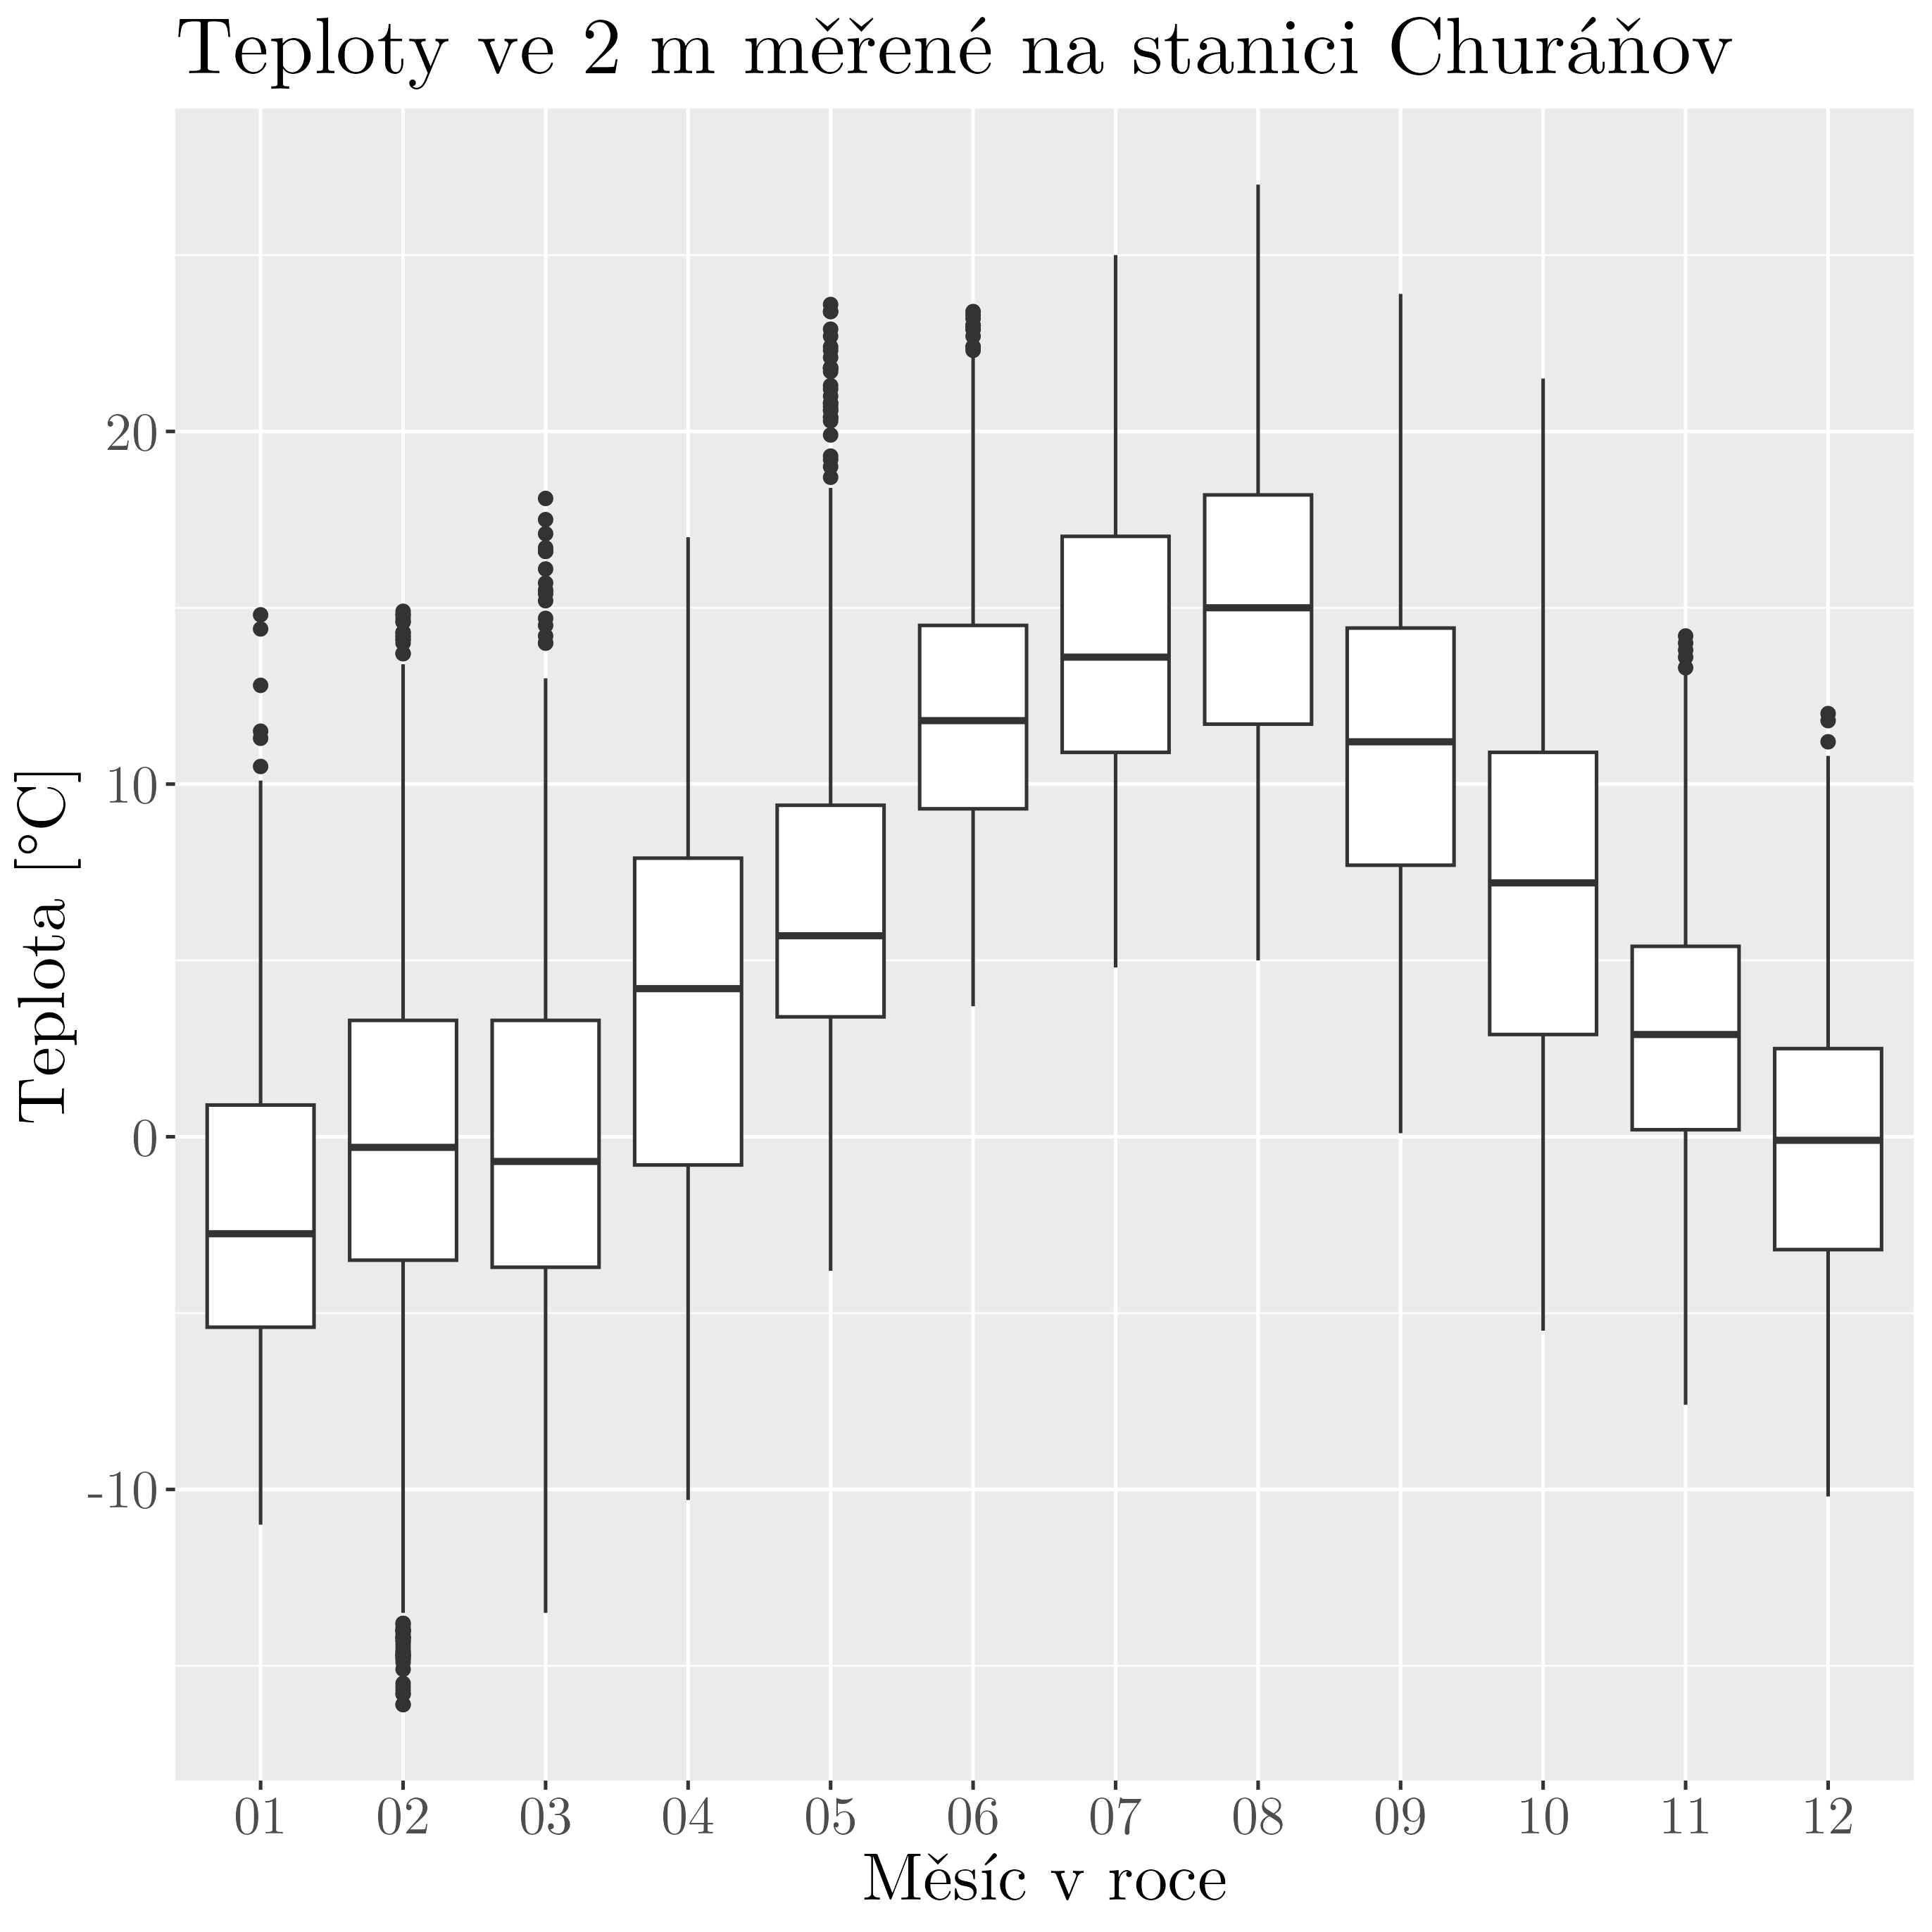
\includegraphics[width=\textwidth]{img/synop_temperature.png}
		\caption{}
		\label{fig:synop_temperature}
	\end{subfigure}
	\hfill
	\begin{subfigure}{0.45\textwidth}
  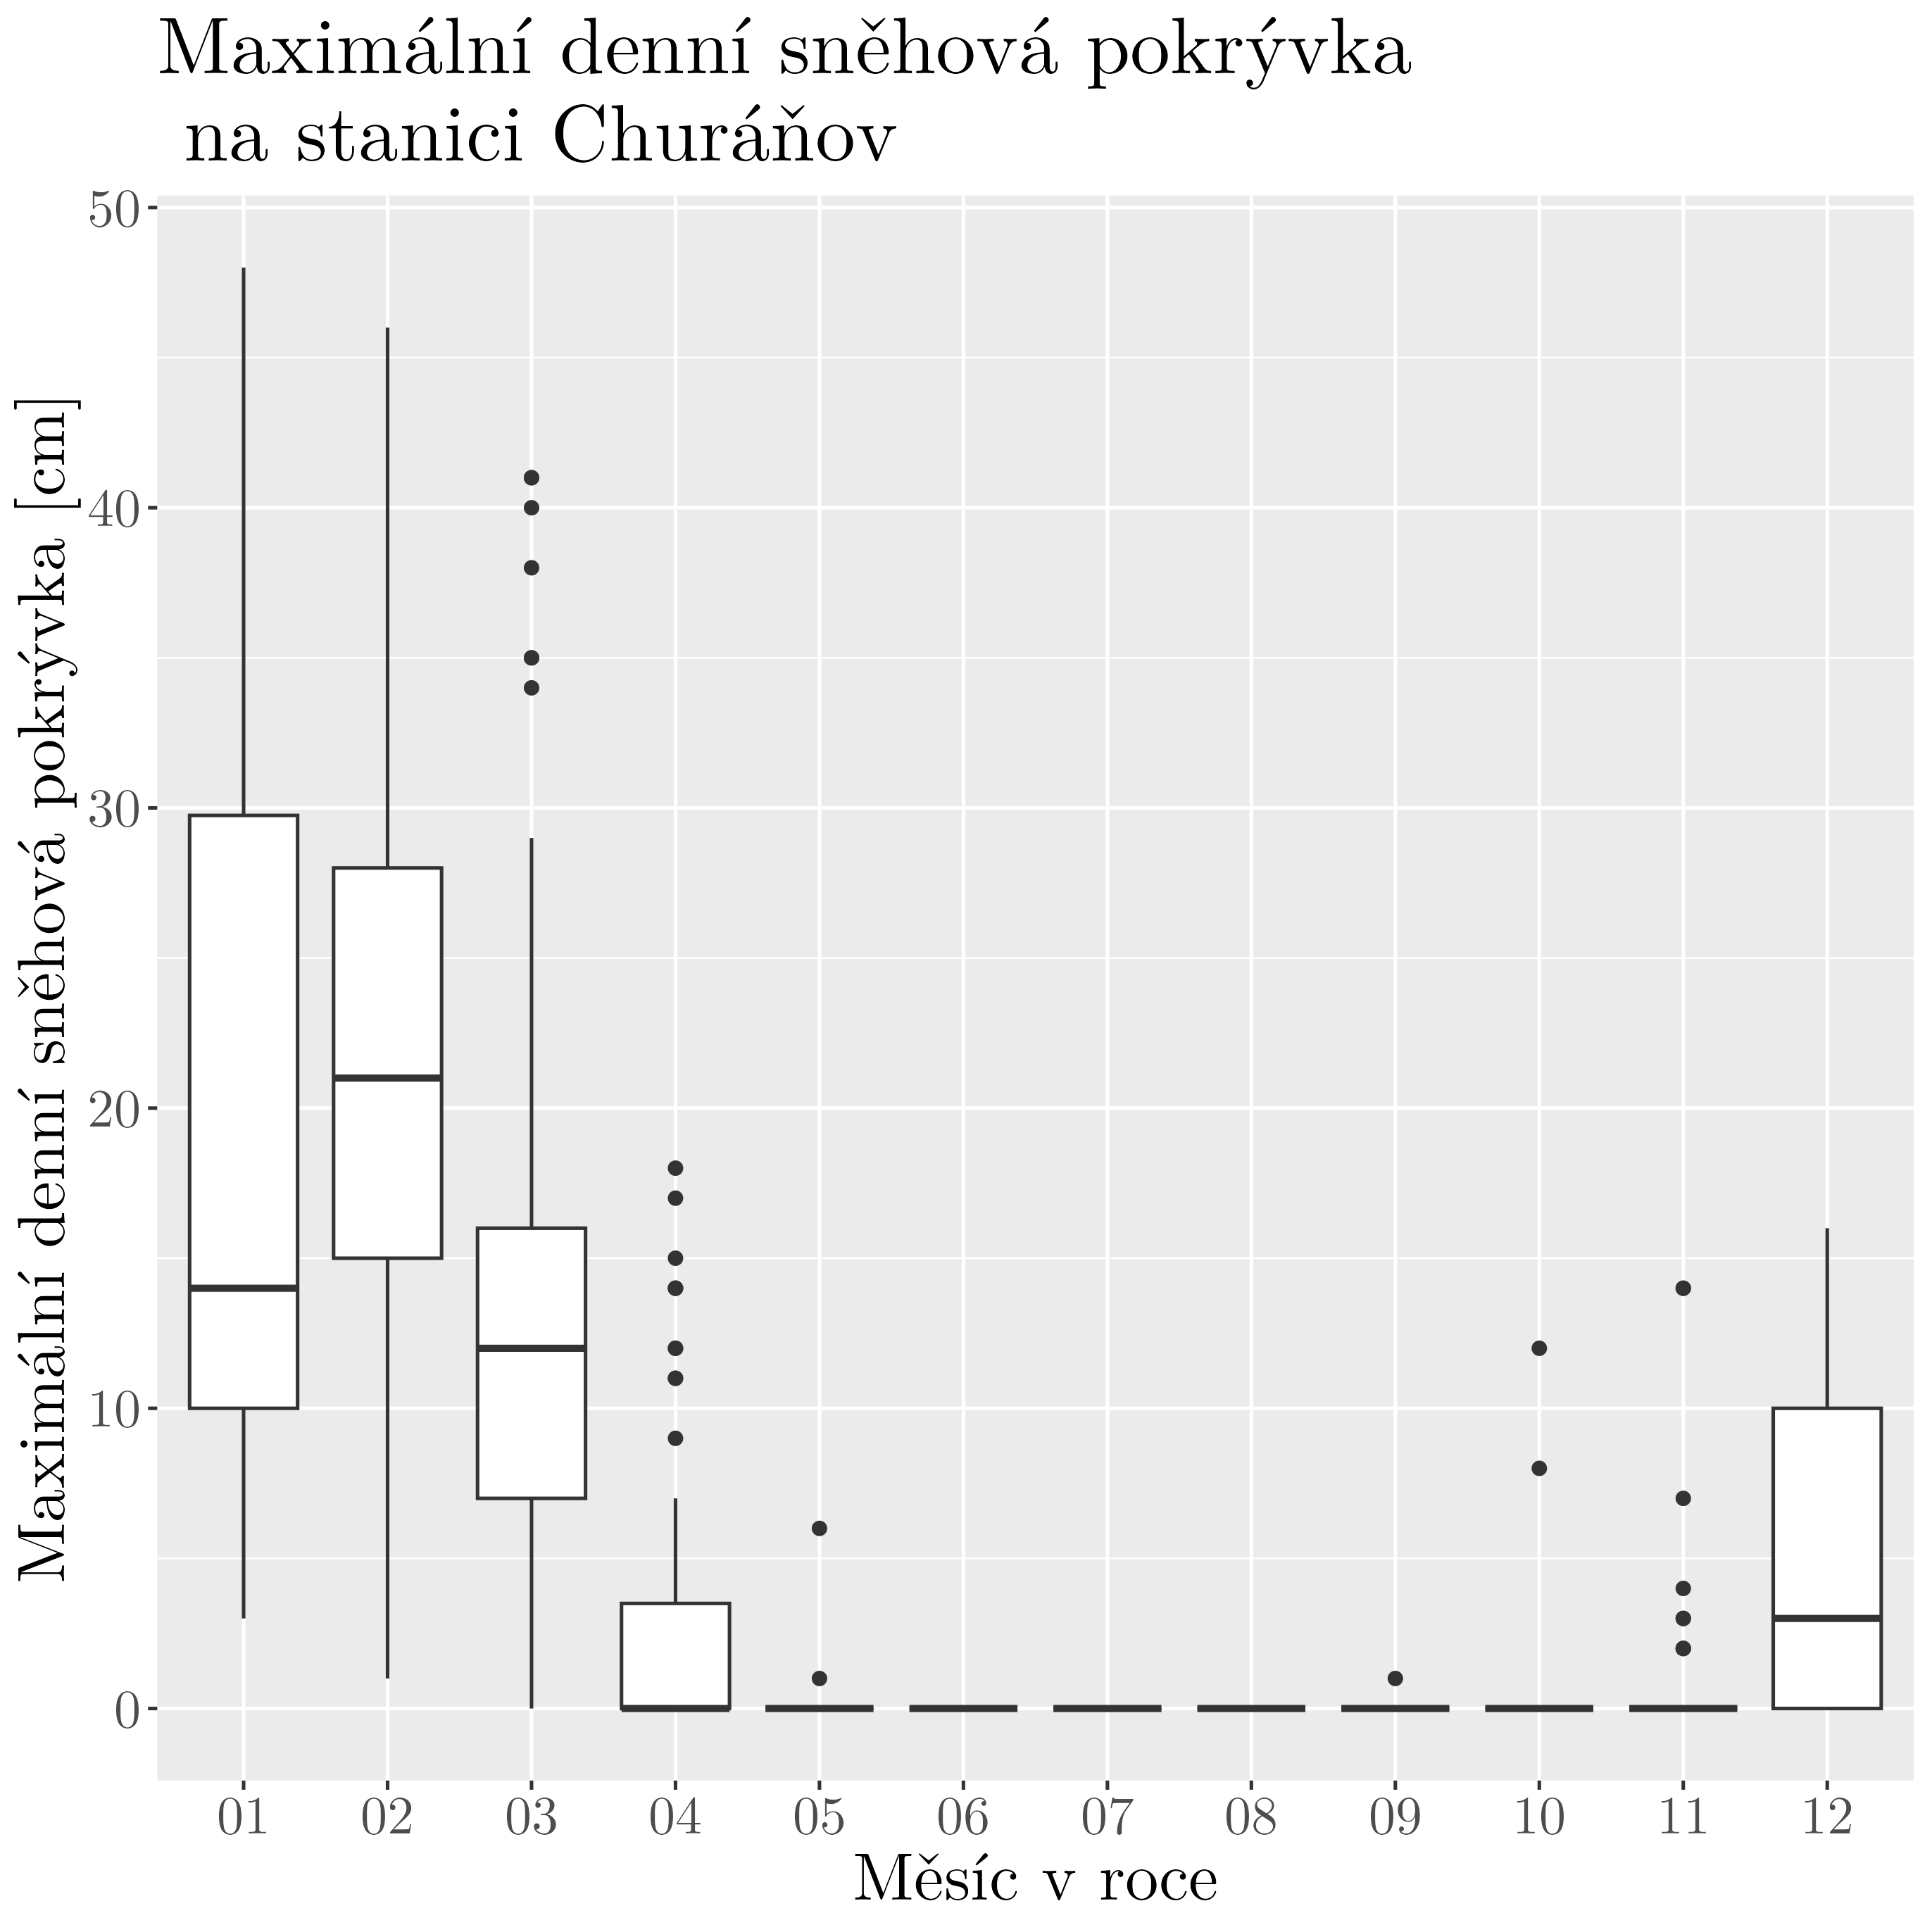
\includegraphics[width=\textwidth]{img/synop_snowcm.png}
		\caption{}
		\label{fig:synop_snowcm}
	\end{subfigure}
	\hfill
	\begin{subfigure}{0.45\textwidth}
  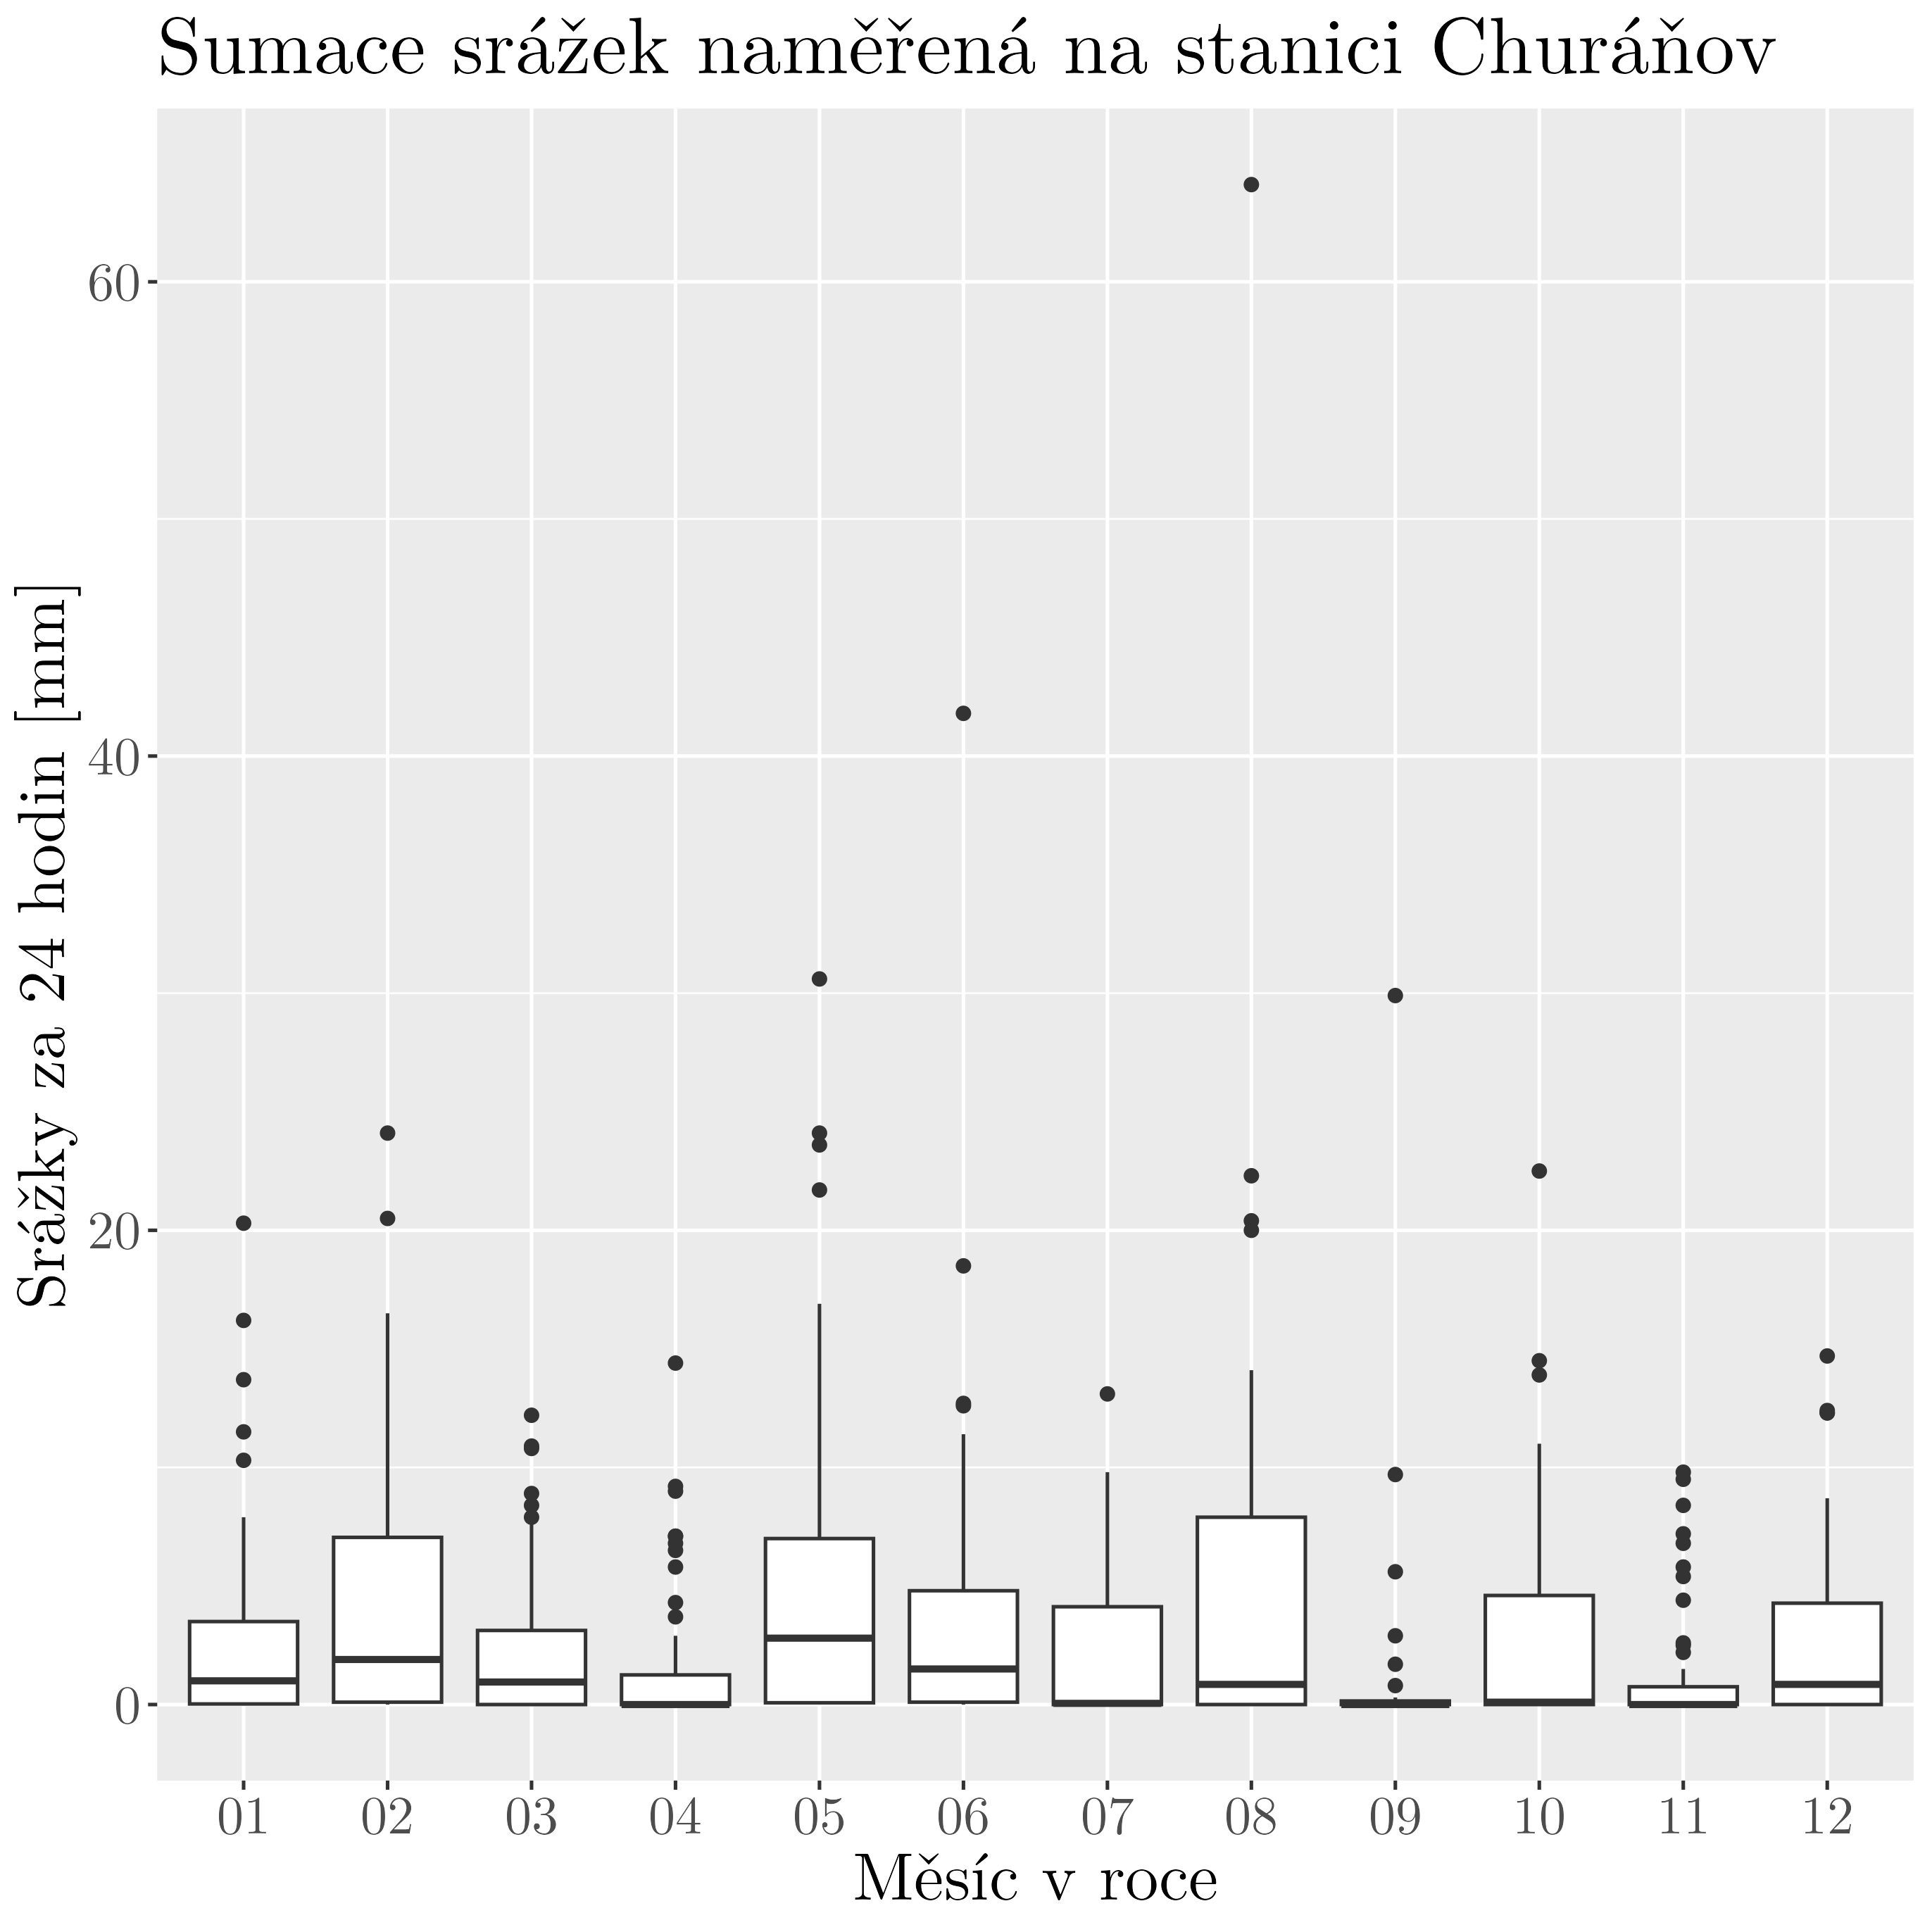
\includegraphics[width=\textwidth]{img/synop_prec.png}
		\caption{}
		\label{fig:synop_prec}
	\end{subfigure}
	\hfill
	\begin{subfigure}{0.45\textwidth}
  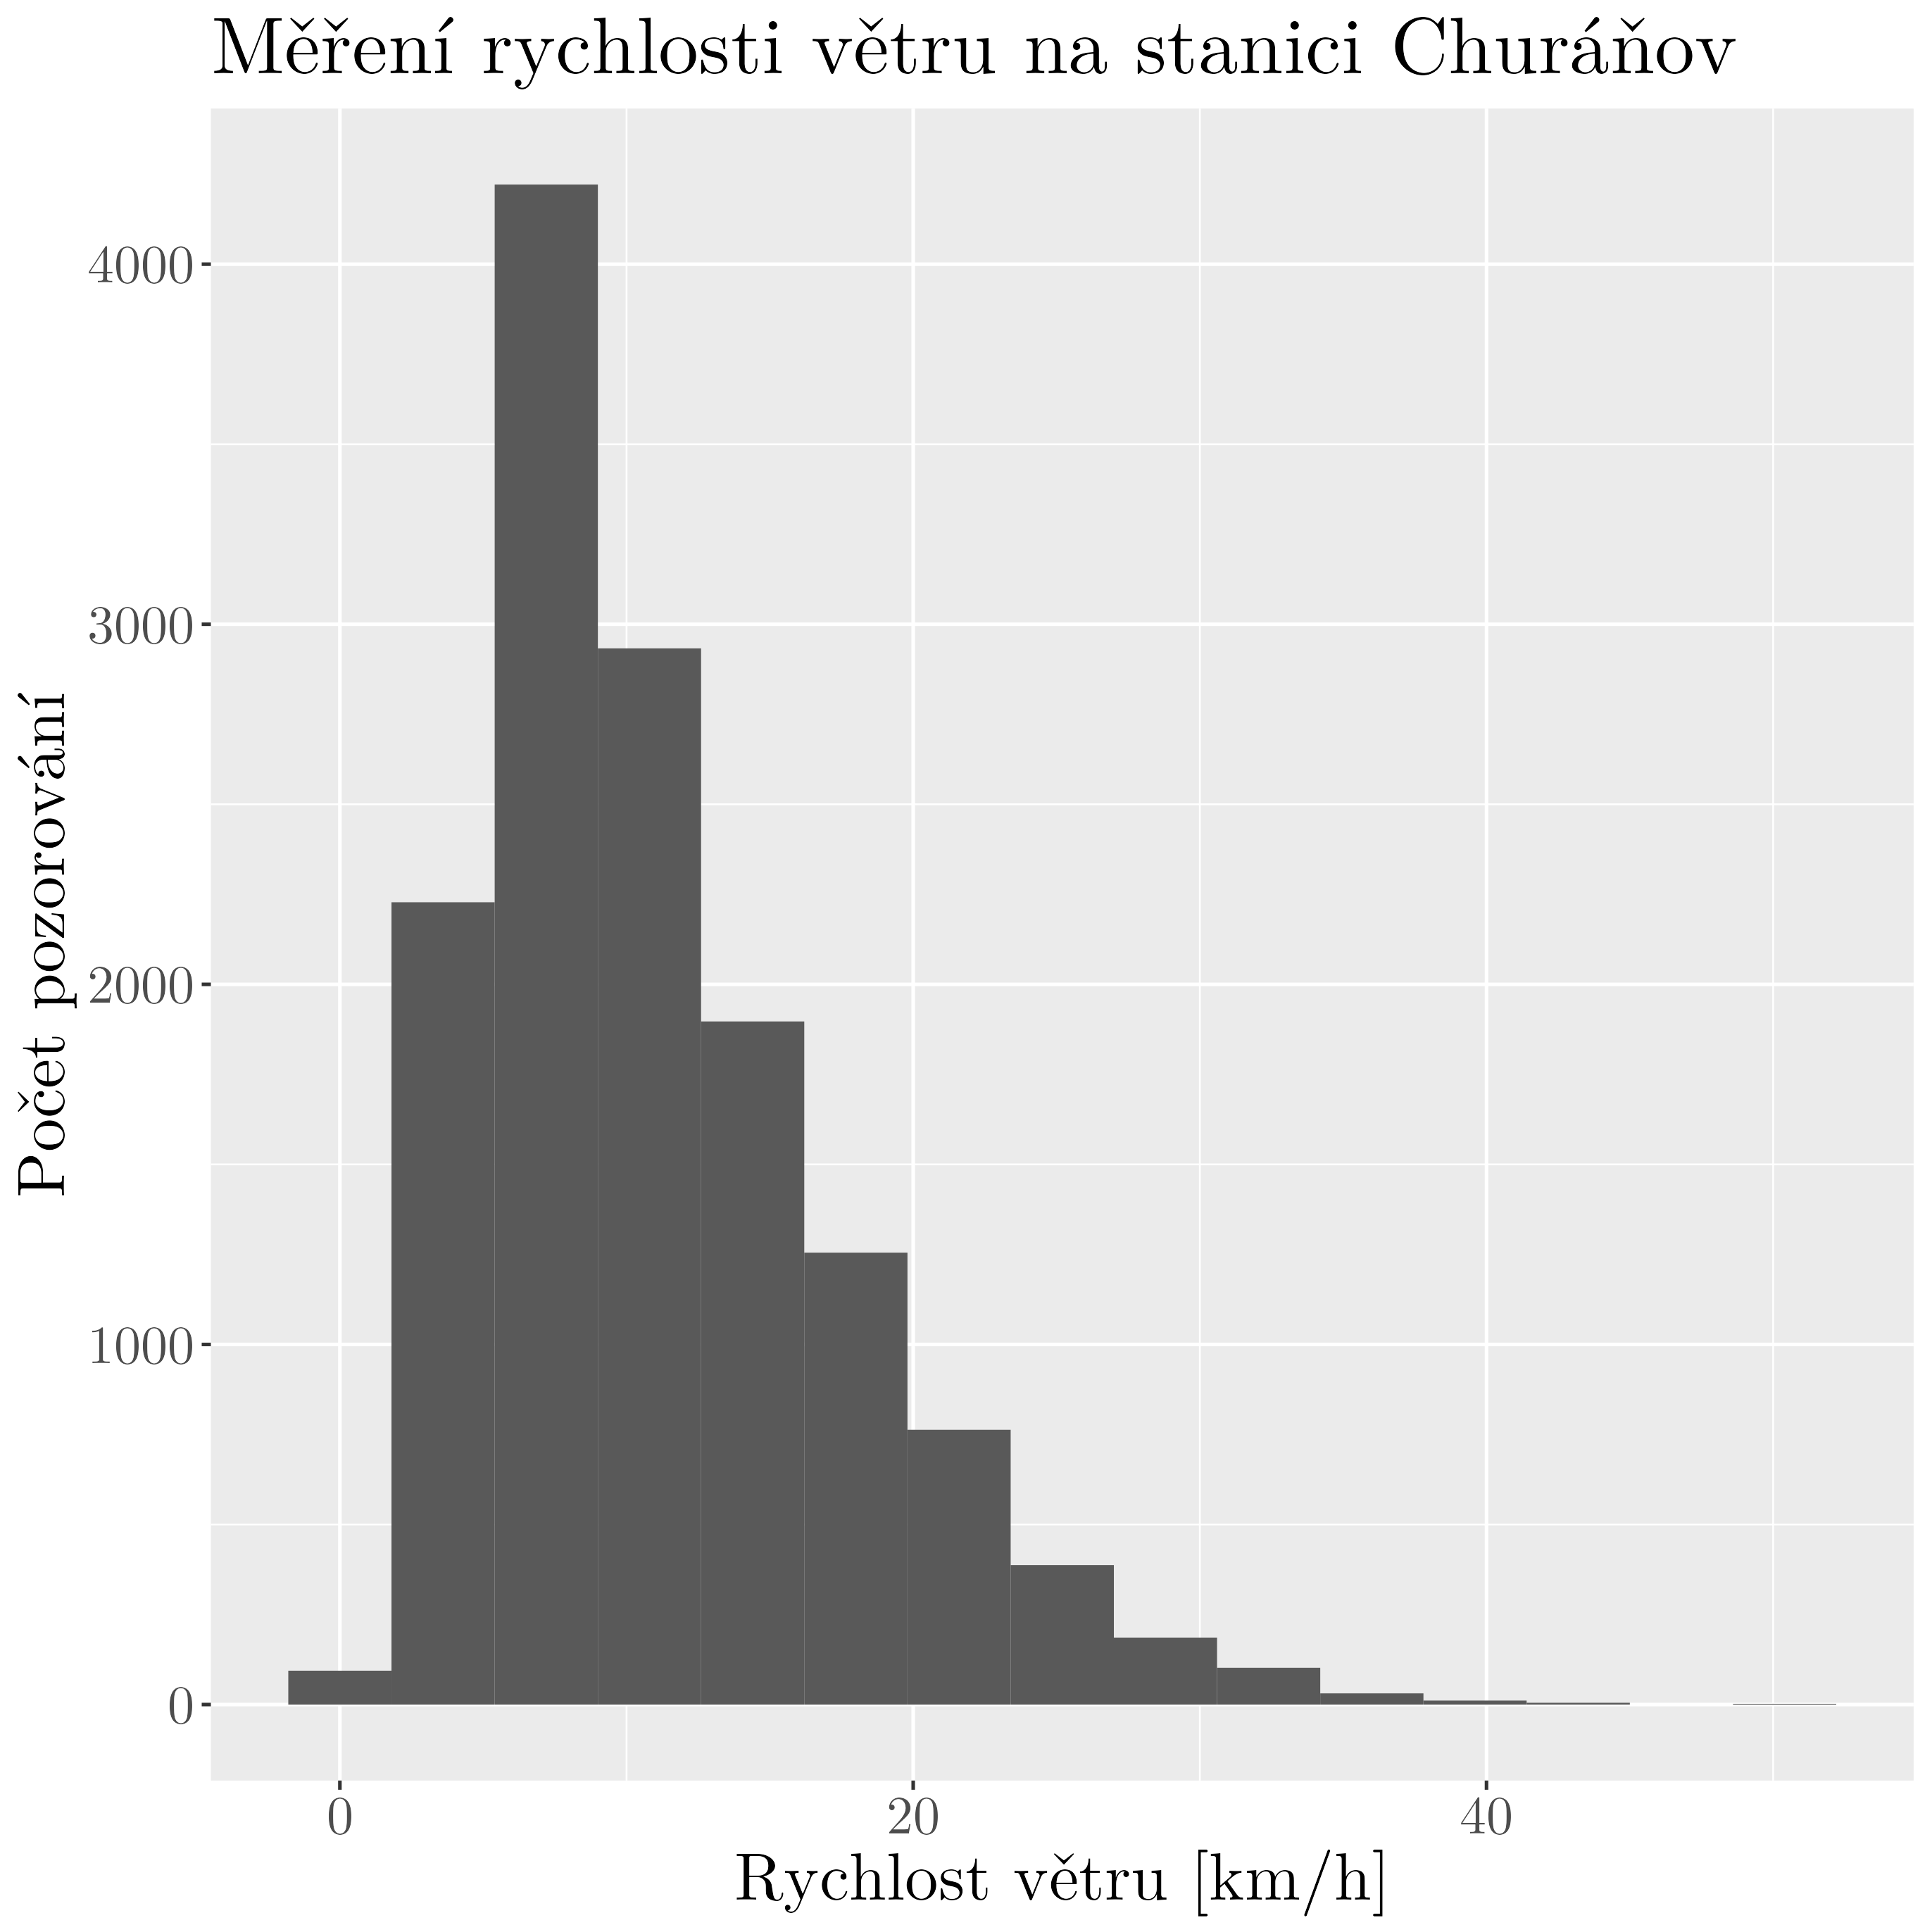
\includegraphics[width=\textwidth]{img/synop_ffkmh.png}
		\caption{}
		\label{fig:synop_ffkmh}
	\end{subfigure}
	\caption{Data ze synoptické stanice Churáňov za období 12.10.2019 až 20.5.2021} 
	\label{fig:chmuukazka}
\end{figure}

\section{Data z BÚ AV}
Data poskytnutá Botanickým ústavem Akademie věd České republiky byla naměřená dvěma typy čidel popisovanými v \ref{chap:loggers}. V části o zpracování dat se budeme zabývat pouze těmi plochami, které jsou opatřeny jak pozemními čidly, tak čidly ve standartní výšce $\SI{2}{m}$. Na obrázku \ref{fig:rozlozenicidel} můžeme vidět jejich prostorové rozložení, celkově jde o 157 čidel. 

Umístění čidel bylo vybíráno tak aby pokryly gradienty nadmořské výšky (5 tříd), potenciální solární radiace (3 třídy) a topografického vlhkostního indexu (3 třídy). Plochy byly dále doplněny tak, aby bylo rovnoměrně pokryto území národních parků a aby se nevyskytovaly poblíž turistických stezek.

\begin{figure}
	\centering
	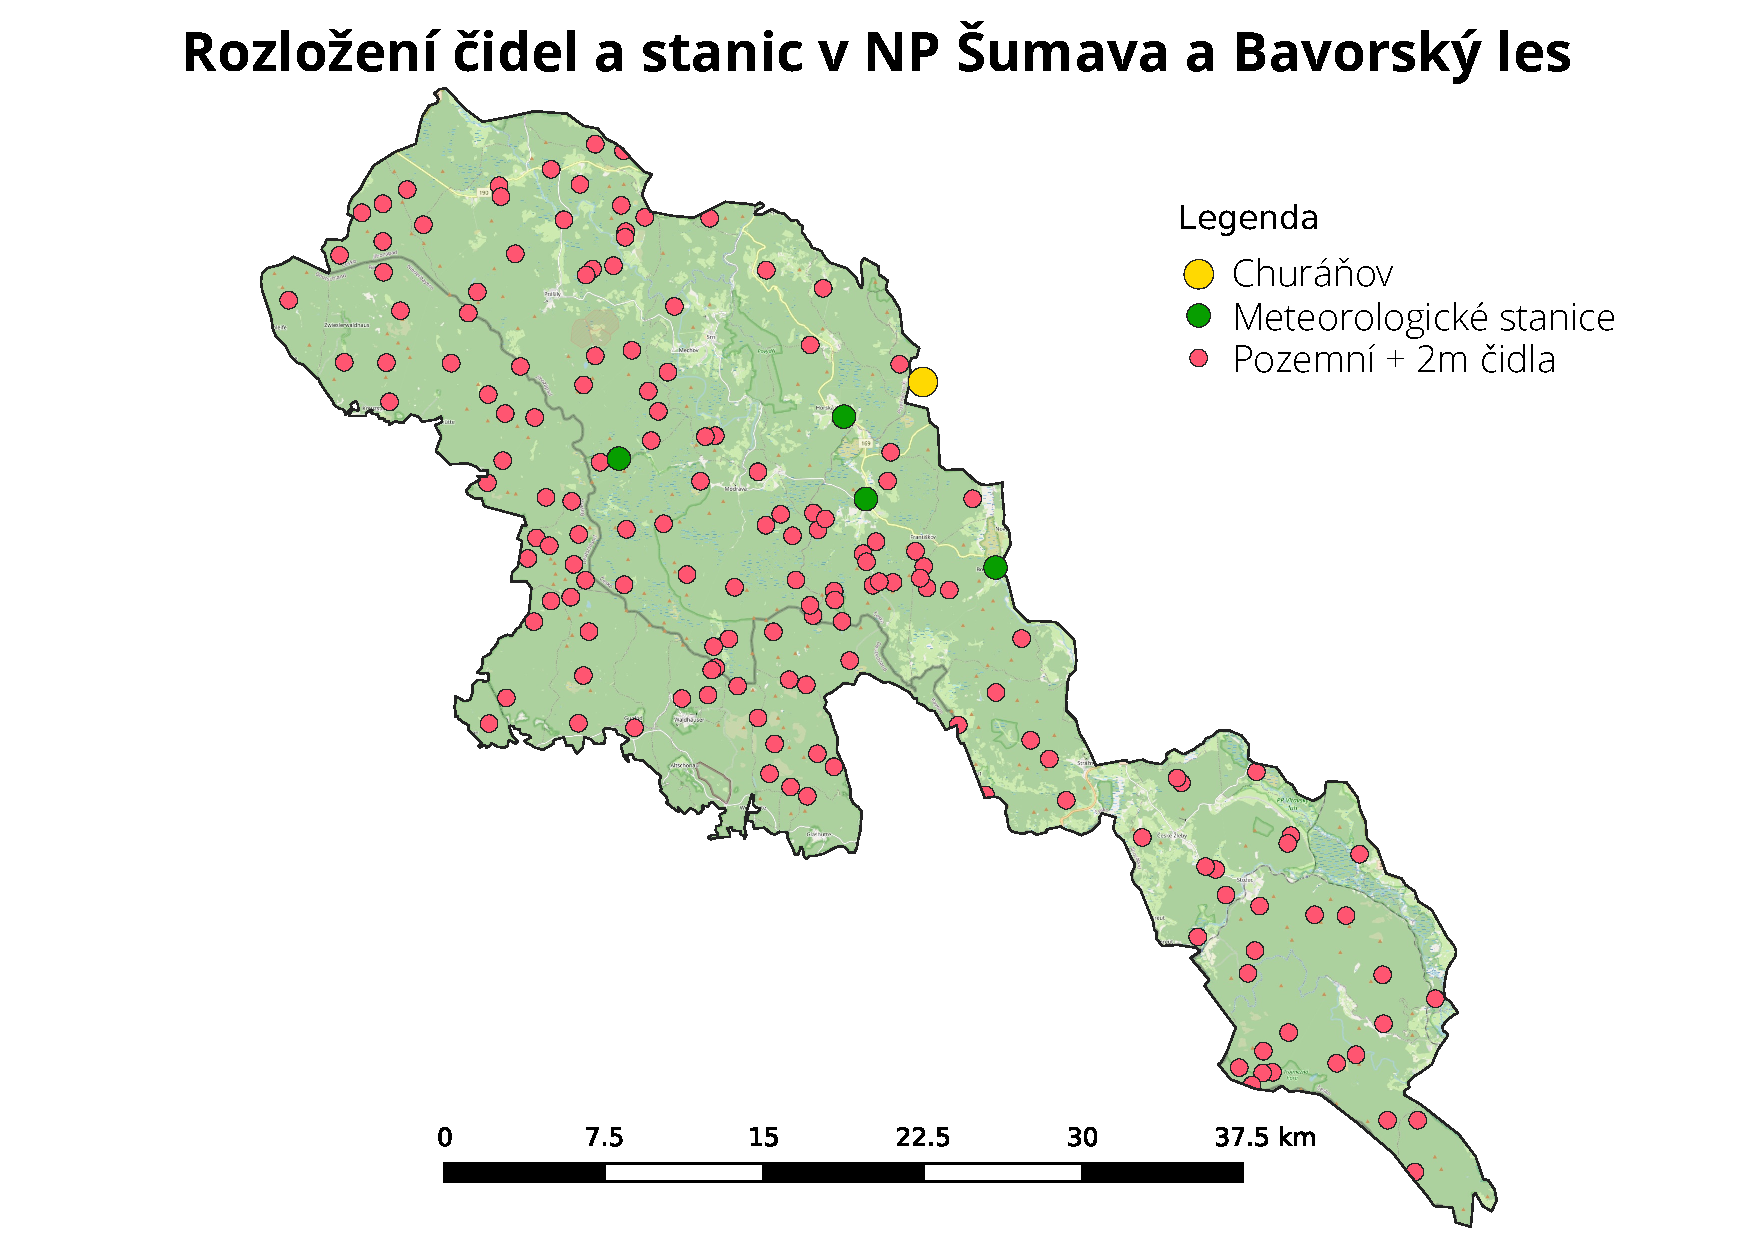
\includegraphics[width=0.95\textwidth]{img/rozlozenicidel.pdf}
	\caption{Rozložení čidel a meteorologický stanic napříč Národním parkem Šumava ($N=112$) a Národním parkem Bavorský les ($N=45$)}
	\label{fig:rozlozenicidel}
\end{figure}

Data vykazují malou chybovost, duplicitní a chybějící záznamy byly vyřazeny. Dále byla data vizuálně překontrolována a části, kdy byla čidla např. povytažená ze země (pozná se podle hodnot půdní vlhkosti), byly nahrazeny hodnotami NA. Podobně pokud čidlo T1 spadlo ze stromu tak jsou hodnoty nahrazeny NA. Toto čištění dat provedli RNDr. Josef Brůna, Ph.D., doc. Ing. Jan Wild, Ph.D. a další s jejichž svolením jsou data využitá v této práci.

Dostupnost dat z čidel je vidět na obrázku \ref{fig:dostupnostdat}, vidíme zde dvě skupiny čidel, jedny, nacházející se v Národním parku Bavorský les mají dostupná data pro cca 400 dnů, zatímco čidla z Národního parku Šumava mají dostupná data pro téměř 600 dnů. Na obrázku \ref{fig:dostupnostdnu} vidíme pak na kolika čidlech jsou zastoupeny jednotlivé dny.

\begin{figure}
	\centering
	\begin{subfigure}{0.45\textwidth}
  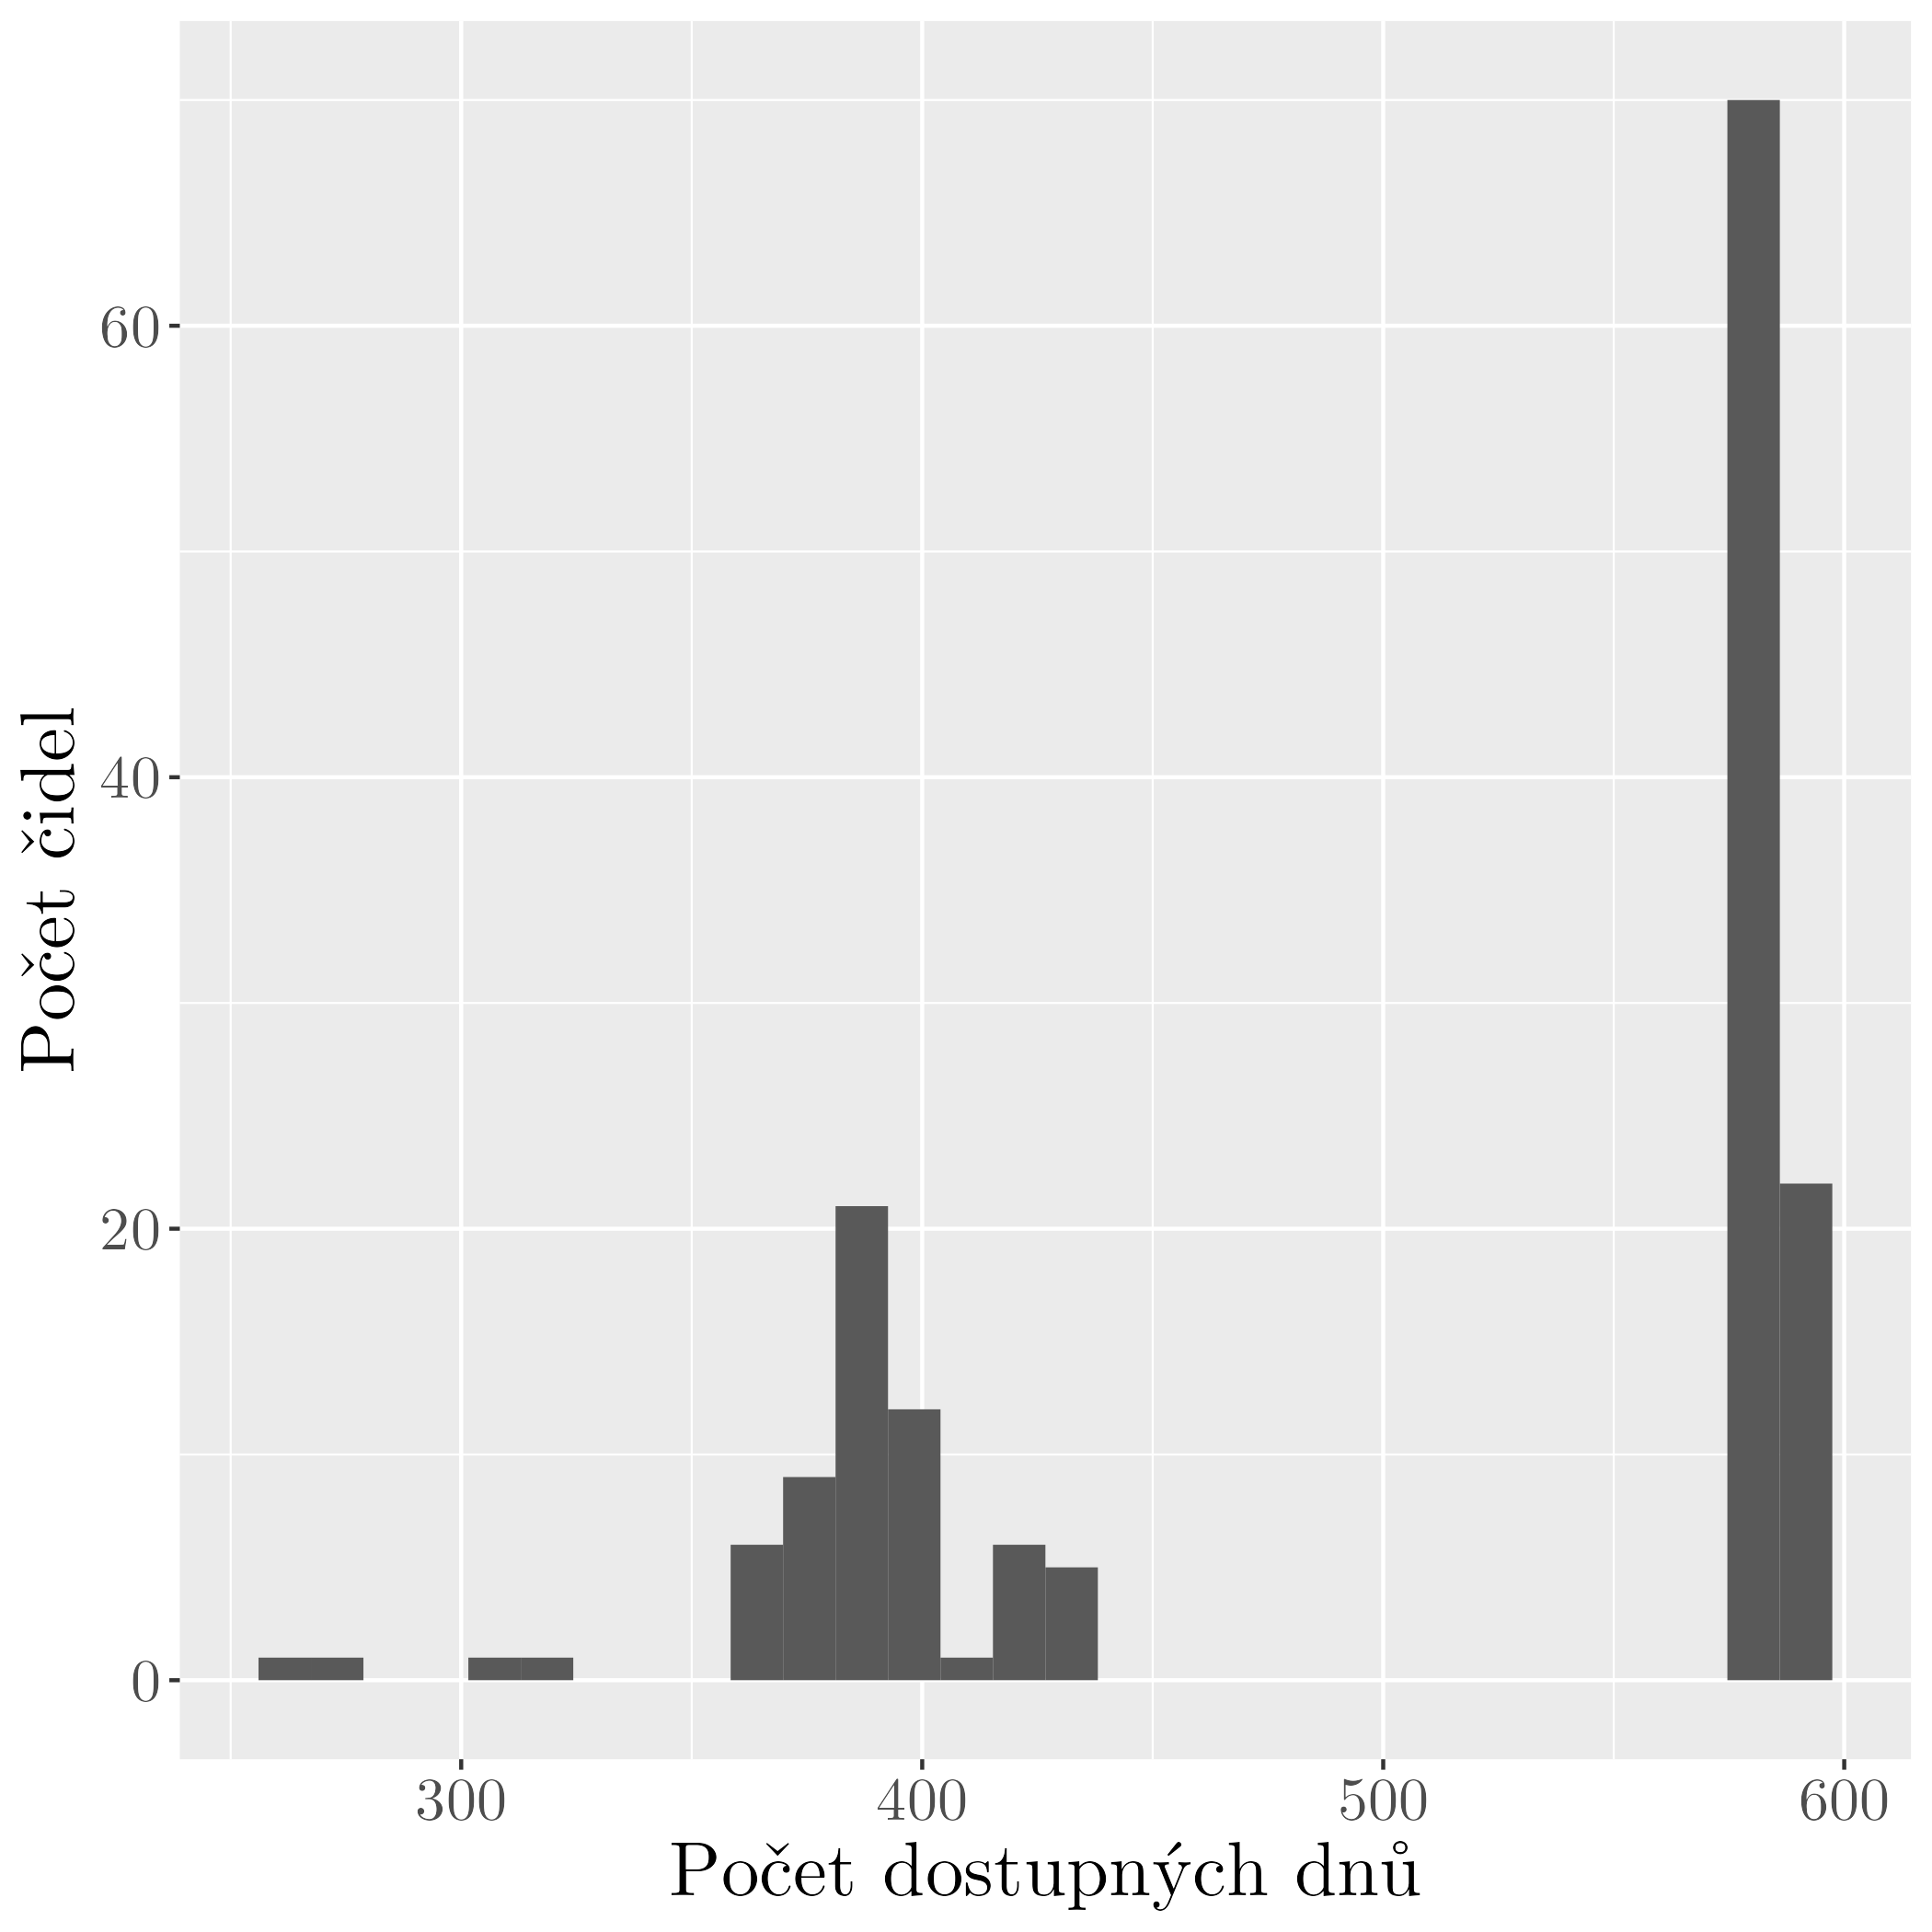
\includegraphics[width=\textwidth]{img/hist_numofdayavailability.png}
	\caption{Histogram ukazující množství dostupných dnů pro jednotlivá čidla}
	\label{fig:dostupnostdat}
	\end{subfigure}
	\hfill
	\begin{subfigure}{0.45\textwidth}
  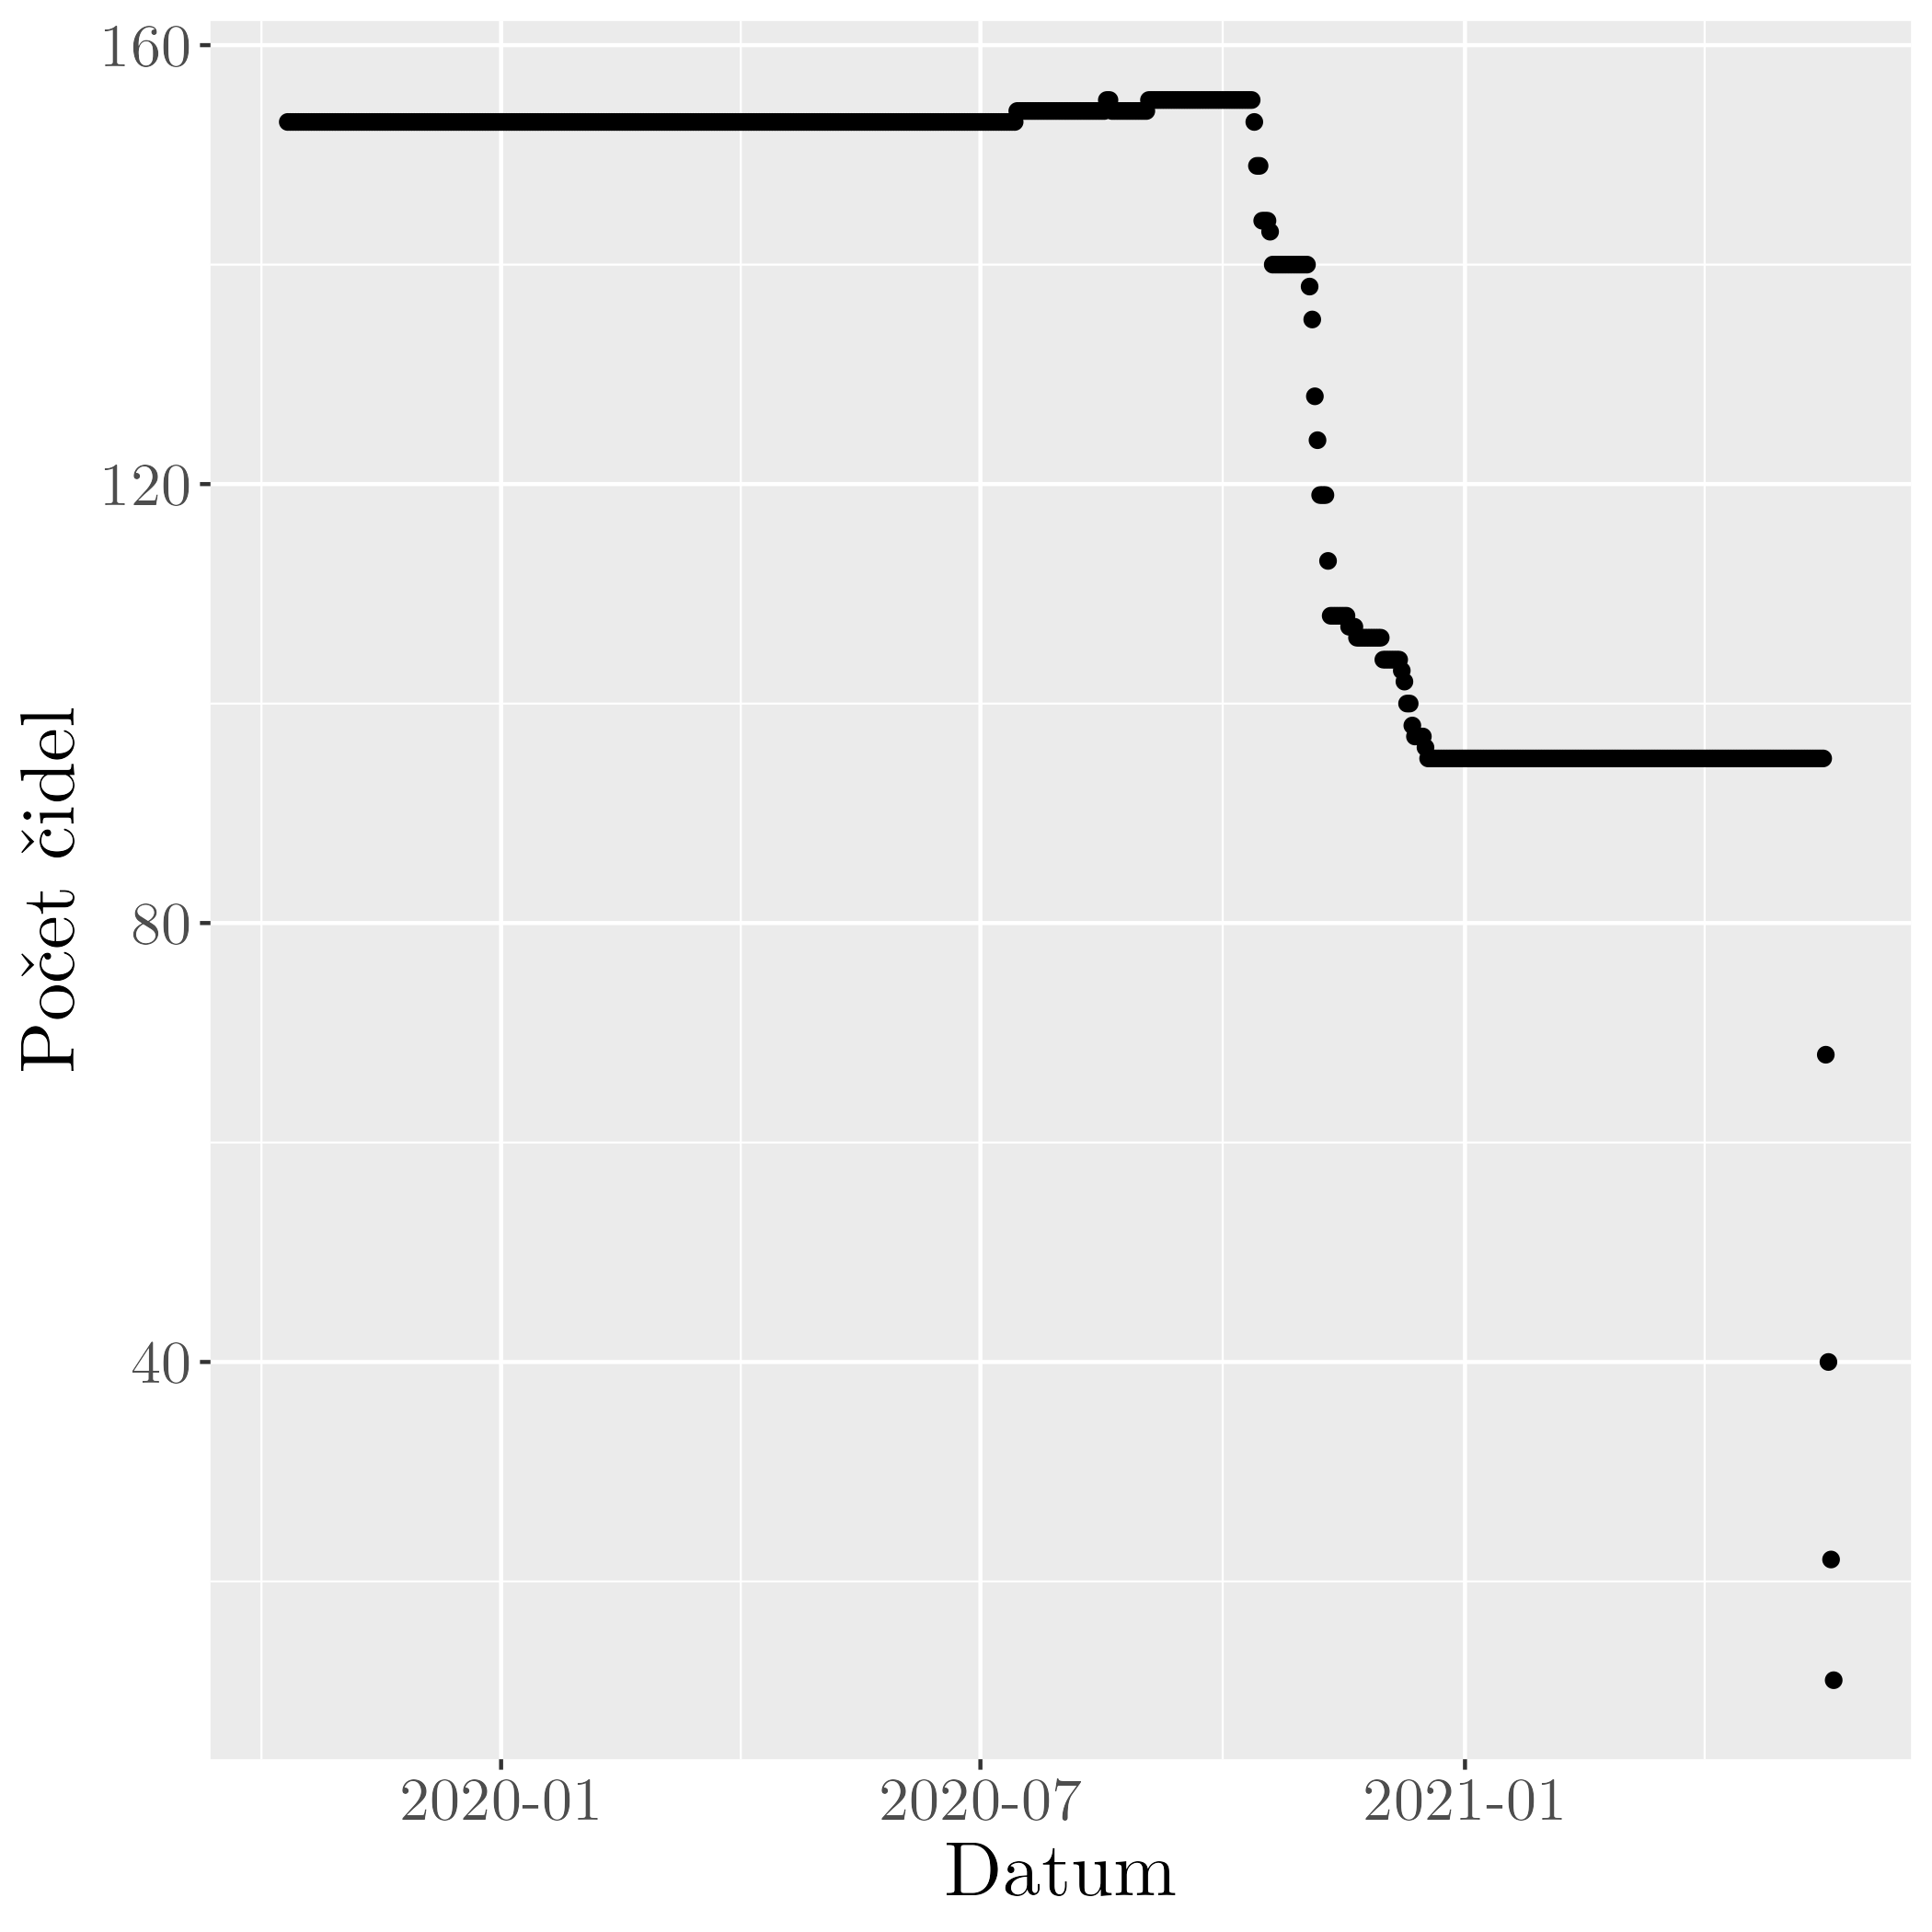
\includegraphics[width=\textwidth]{img/date_availability.png}
	\caption{Graf zastoupení čidel pro jednotlivé dny}
	\label{fig:dostupnostdnu}
	\end{subfigure}
	\caption{Dostupnost dat z čidel}
\end{figure}

\section{Ukázky použitých dat}
Dále se podívejme na ukázku dat naměřených na čidlech. Na obrázcích \ref{fig:hours} můžeme vidět kdy nastávaly maximální a minimální teploty ve výškách $\SI{0}{cm}$ a $\SI{15}{cm}$ nad zemí, denní hodina je uvedená v UTC, nikoliv SEČ nebo SELČ. U maximálních teplot si můžeme všimnout kromě maxima v okolí 10 UTC také menšího maxima a odlehlých hodnot způsobených přítomností sněhu v zimě. Podobně měl sníh vliv i na dobu minimálních teplot v zimě.

\begin{figure}
	\centering
	\begin{subfigure}{0.45\textwidth}
  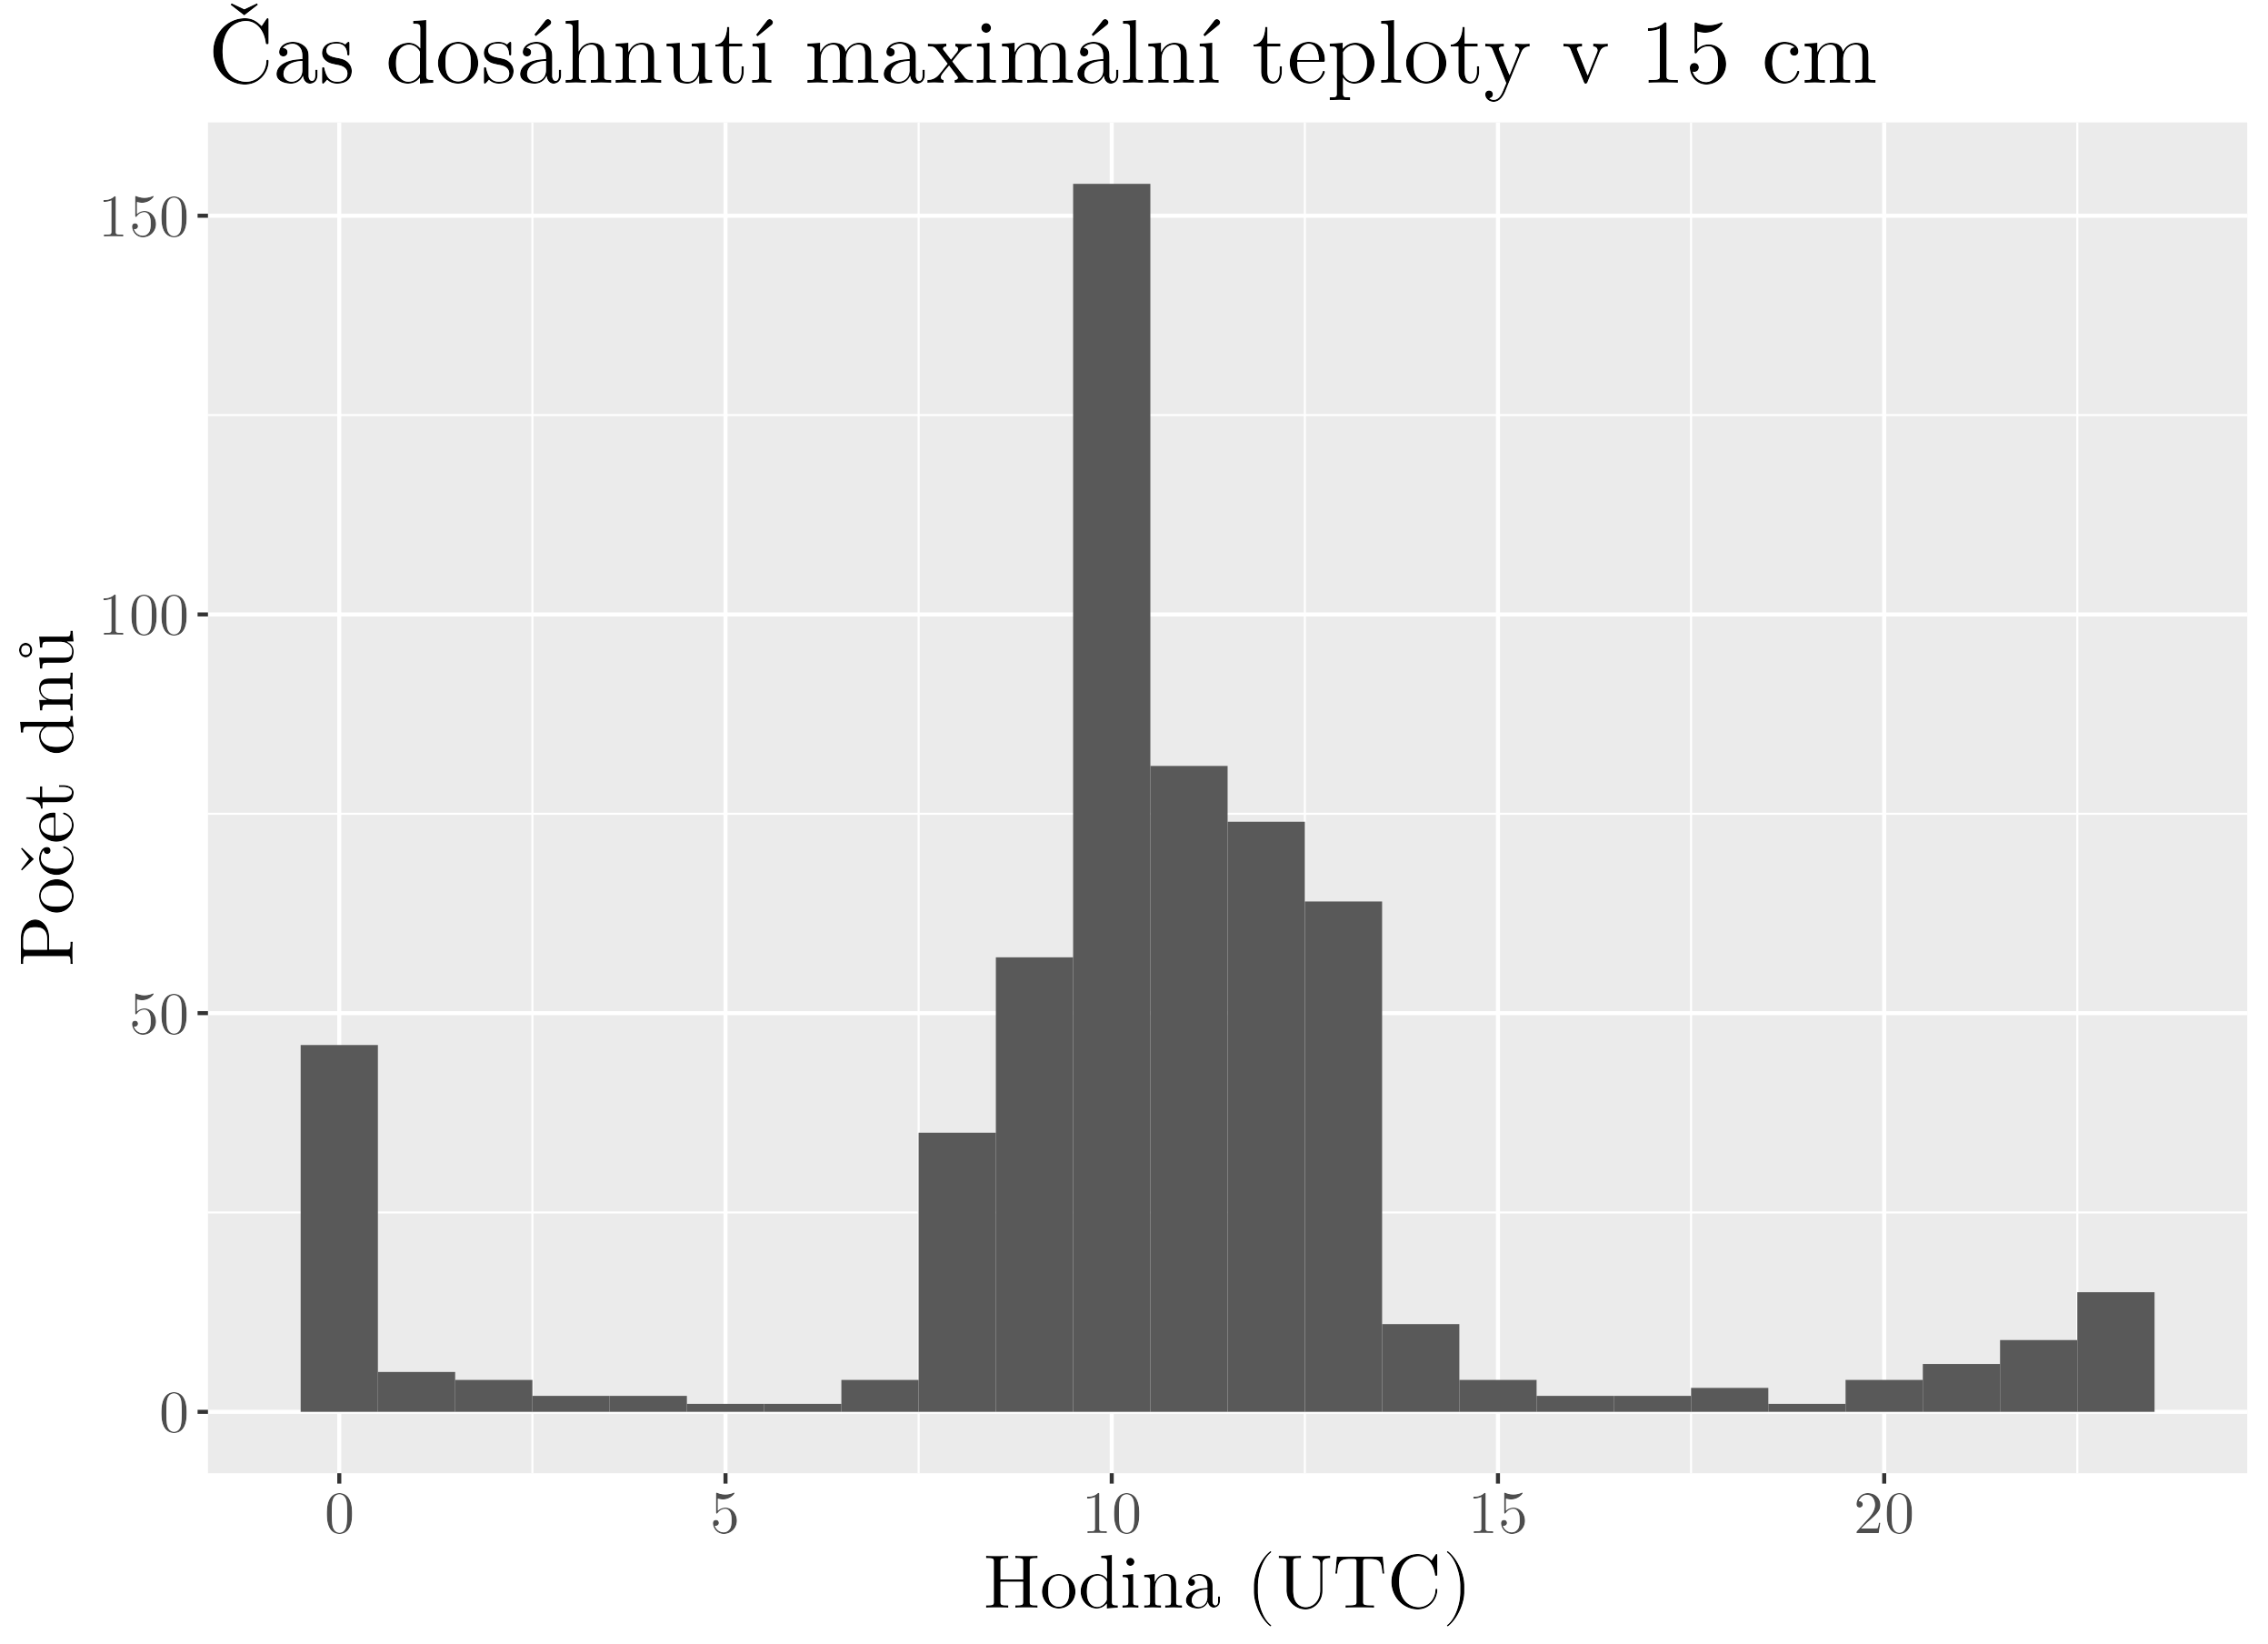
\includegraphics[width=\textwidth]{img/hist_hourmax15cm.png}
		\caption{}
		\label{fig:hourmax15cm}
	\end{subfigure}
	\hfill
	\begin{subfigure}{0.45\textwidth}
  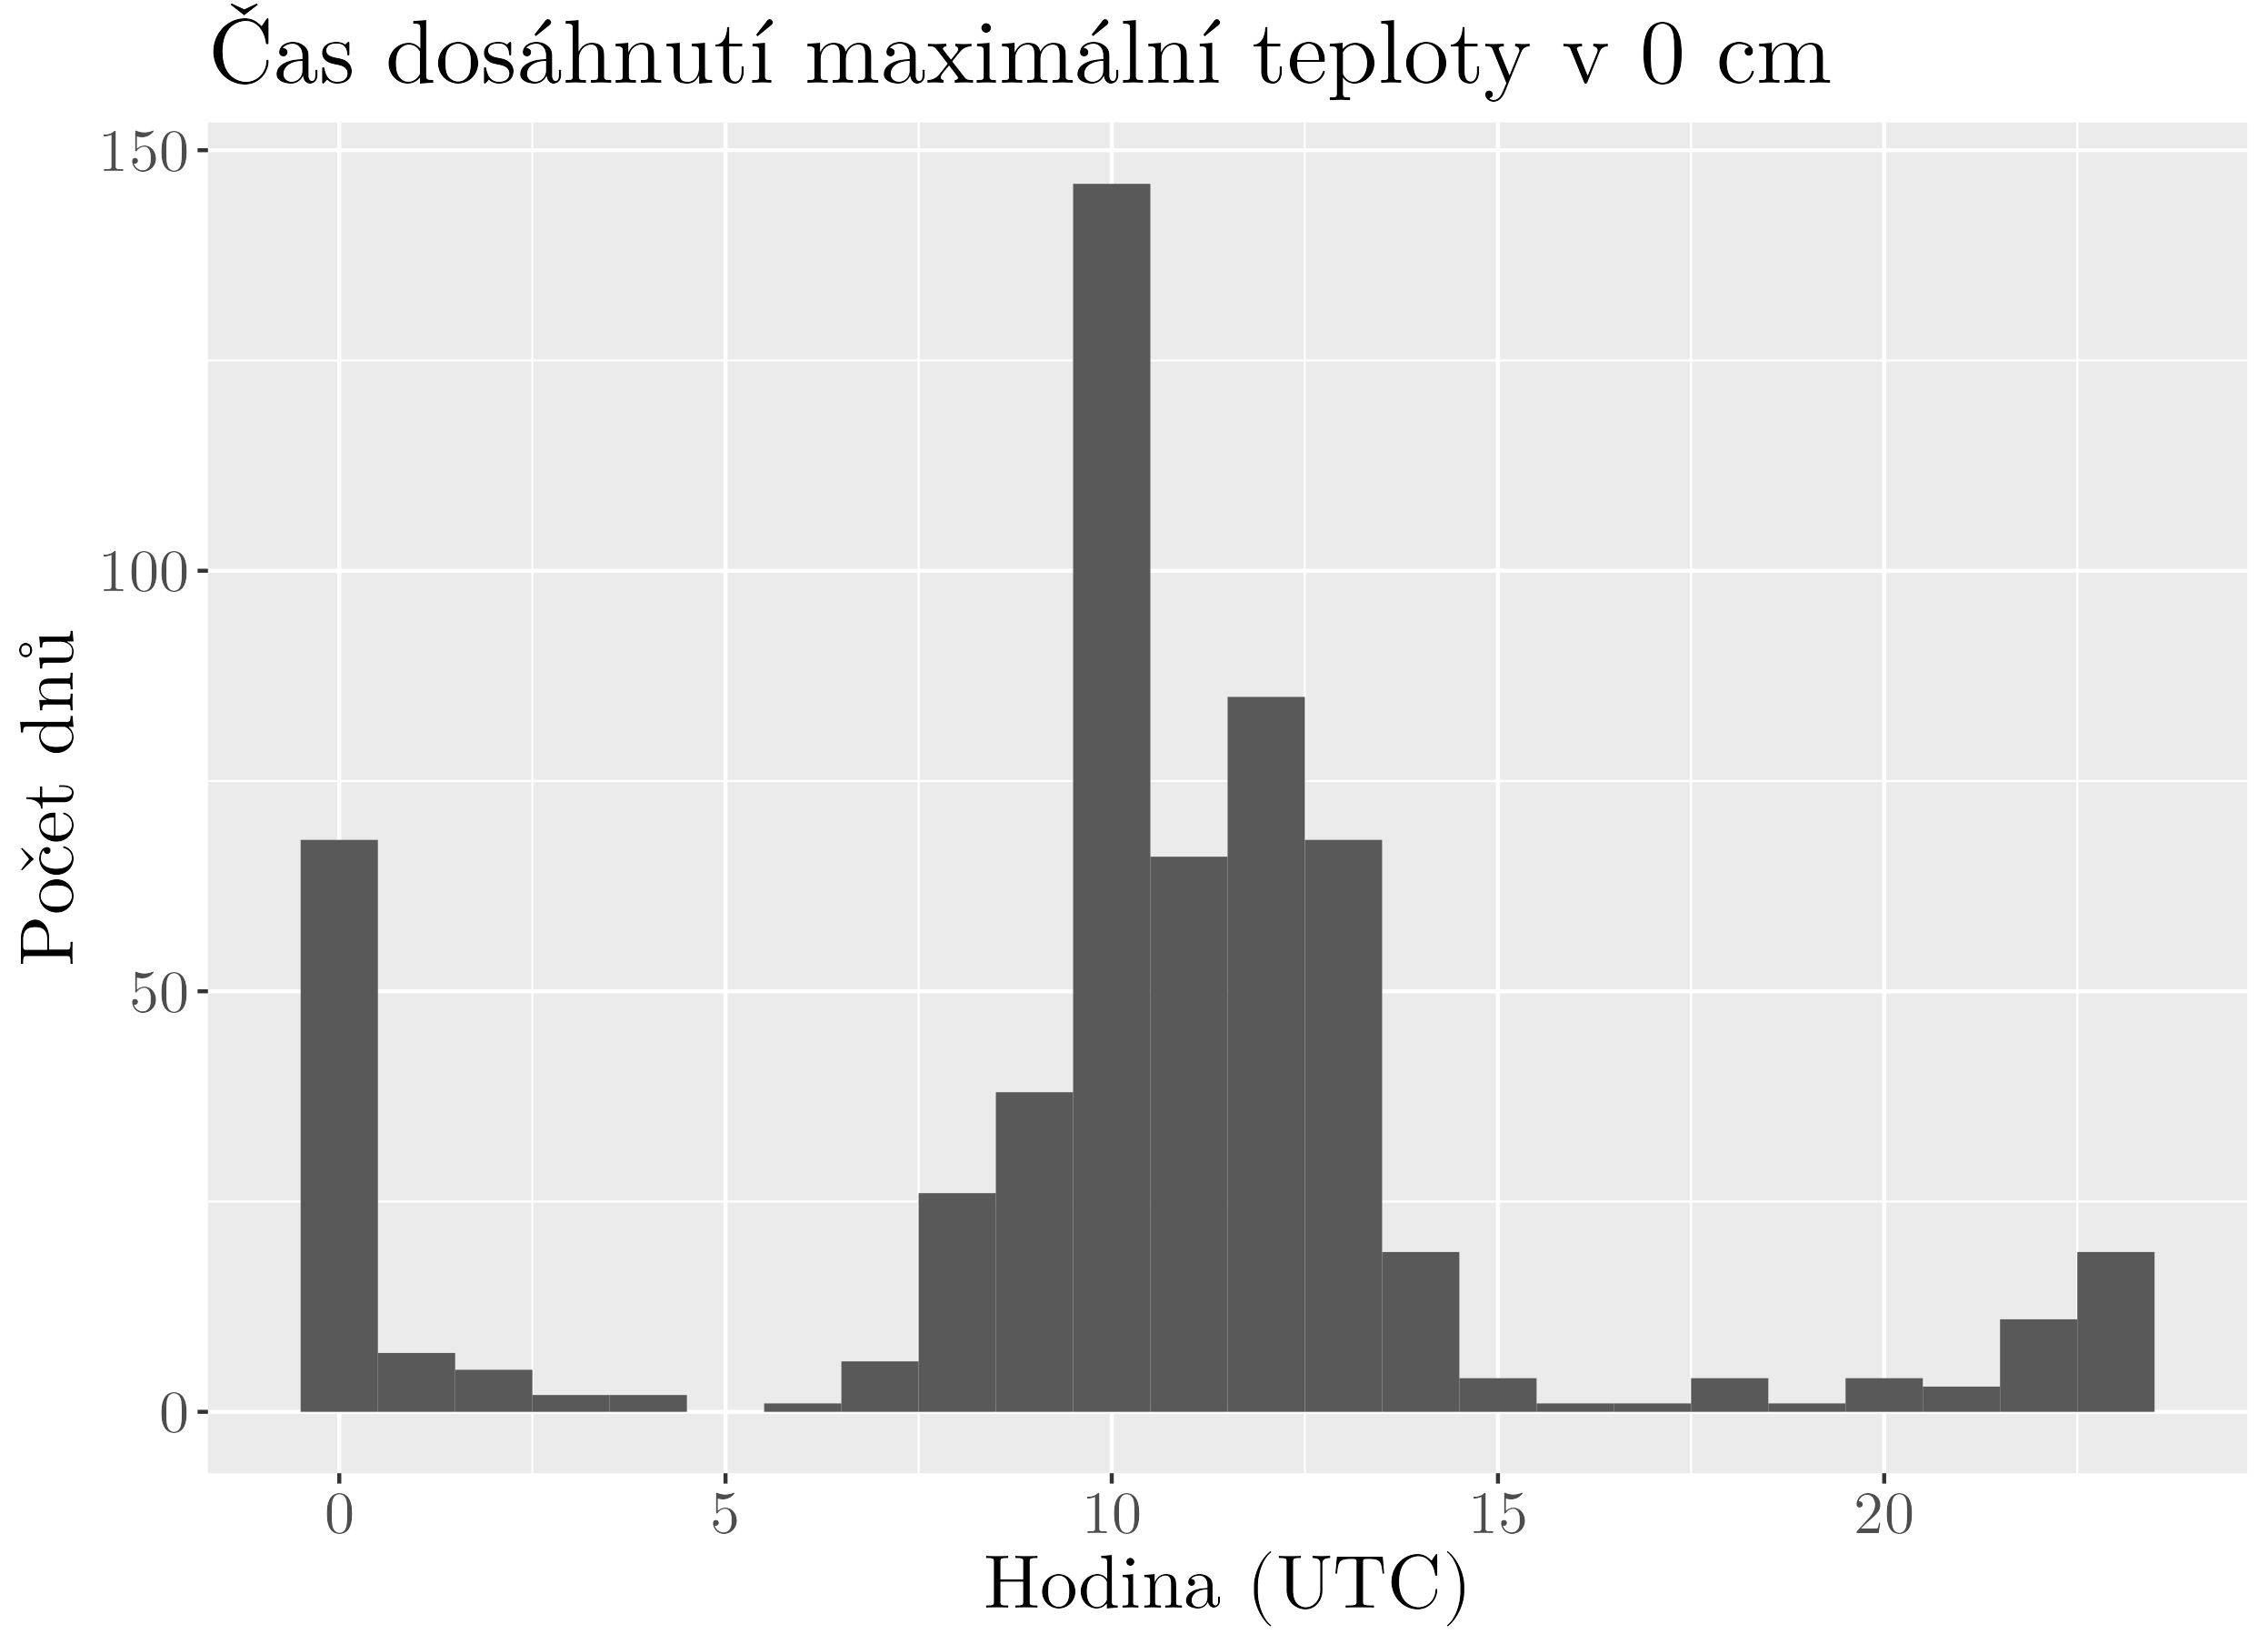
\includegraphics[width=\textwidth]{img/hist_hourmax0cm.png}
		\caption{}
		\label{fig:hourmax0cm}
	\end{subfigure}
	\hfill
	\begin{subfigure}{0.45\textwidth}
  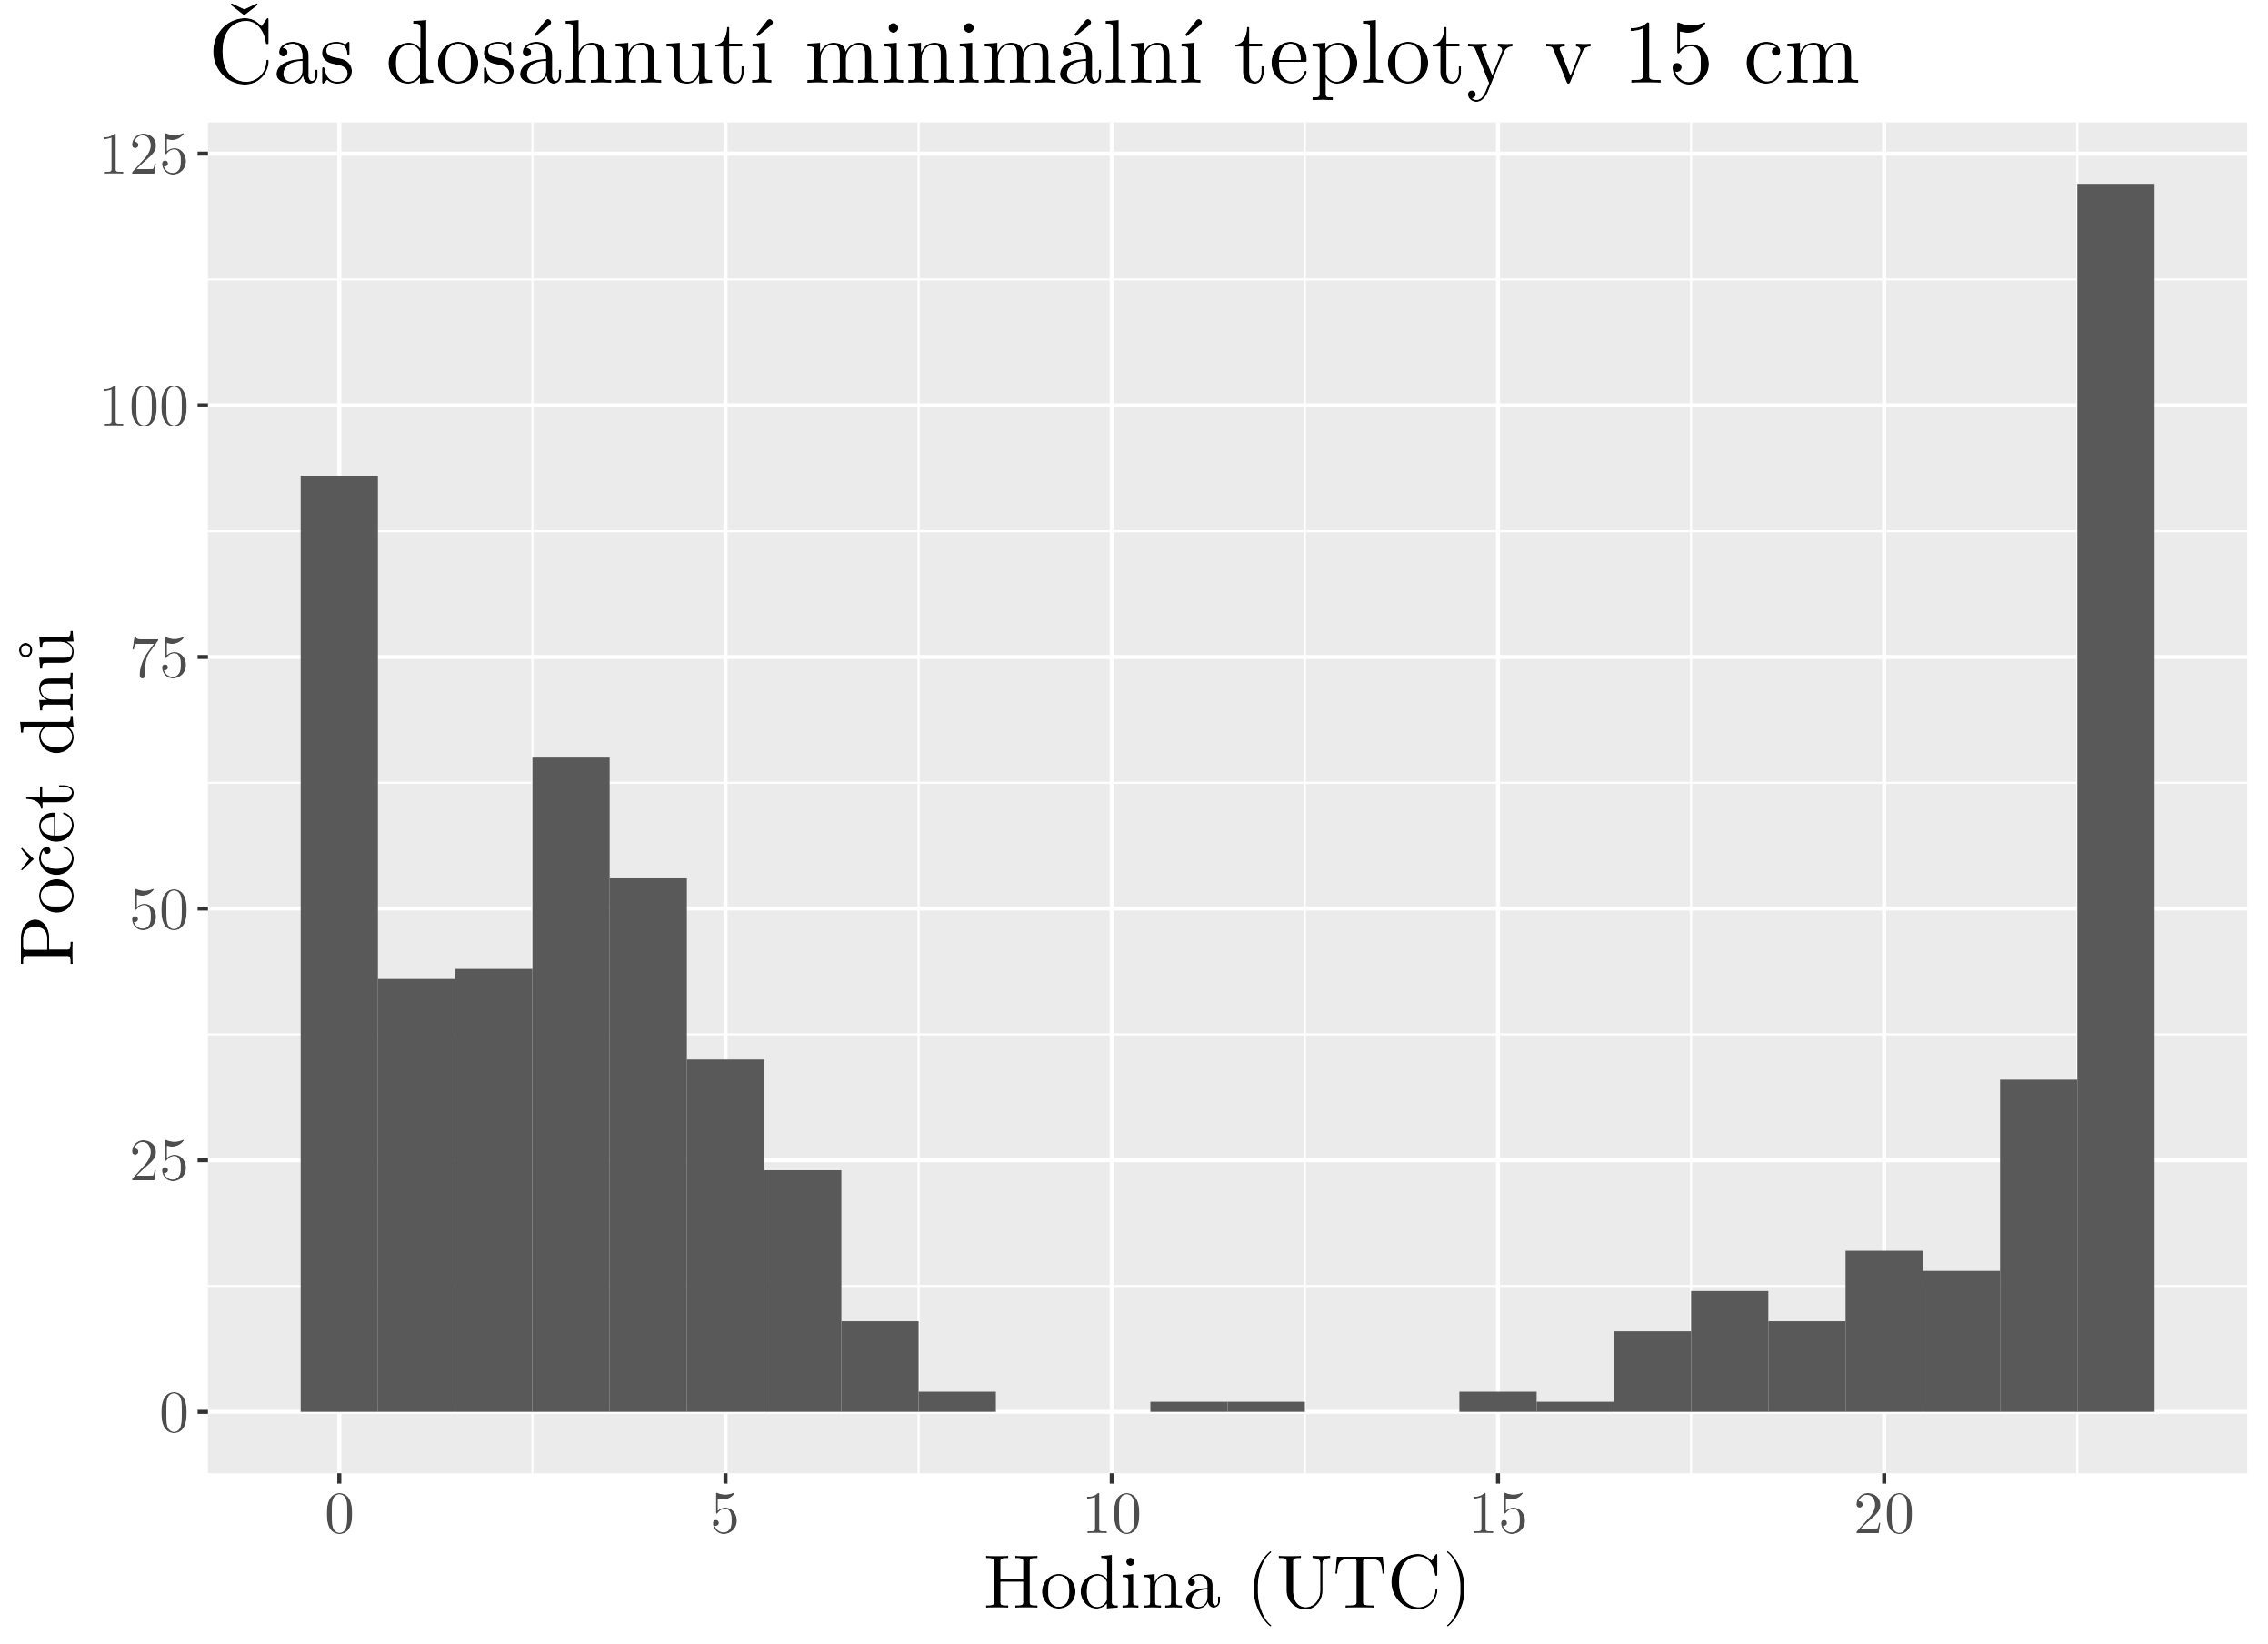
\includegraphics[width=\textwidth]{img/hist_hourmin15cm.png}
		\caption{}
		\label{fig:hourmin15cm}
	\end{subfigure}
	\hfill
	\begin{subfigure}{0.45\textwidth}
  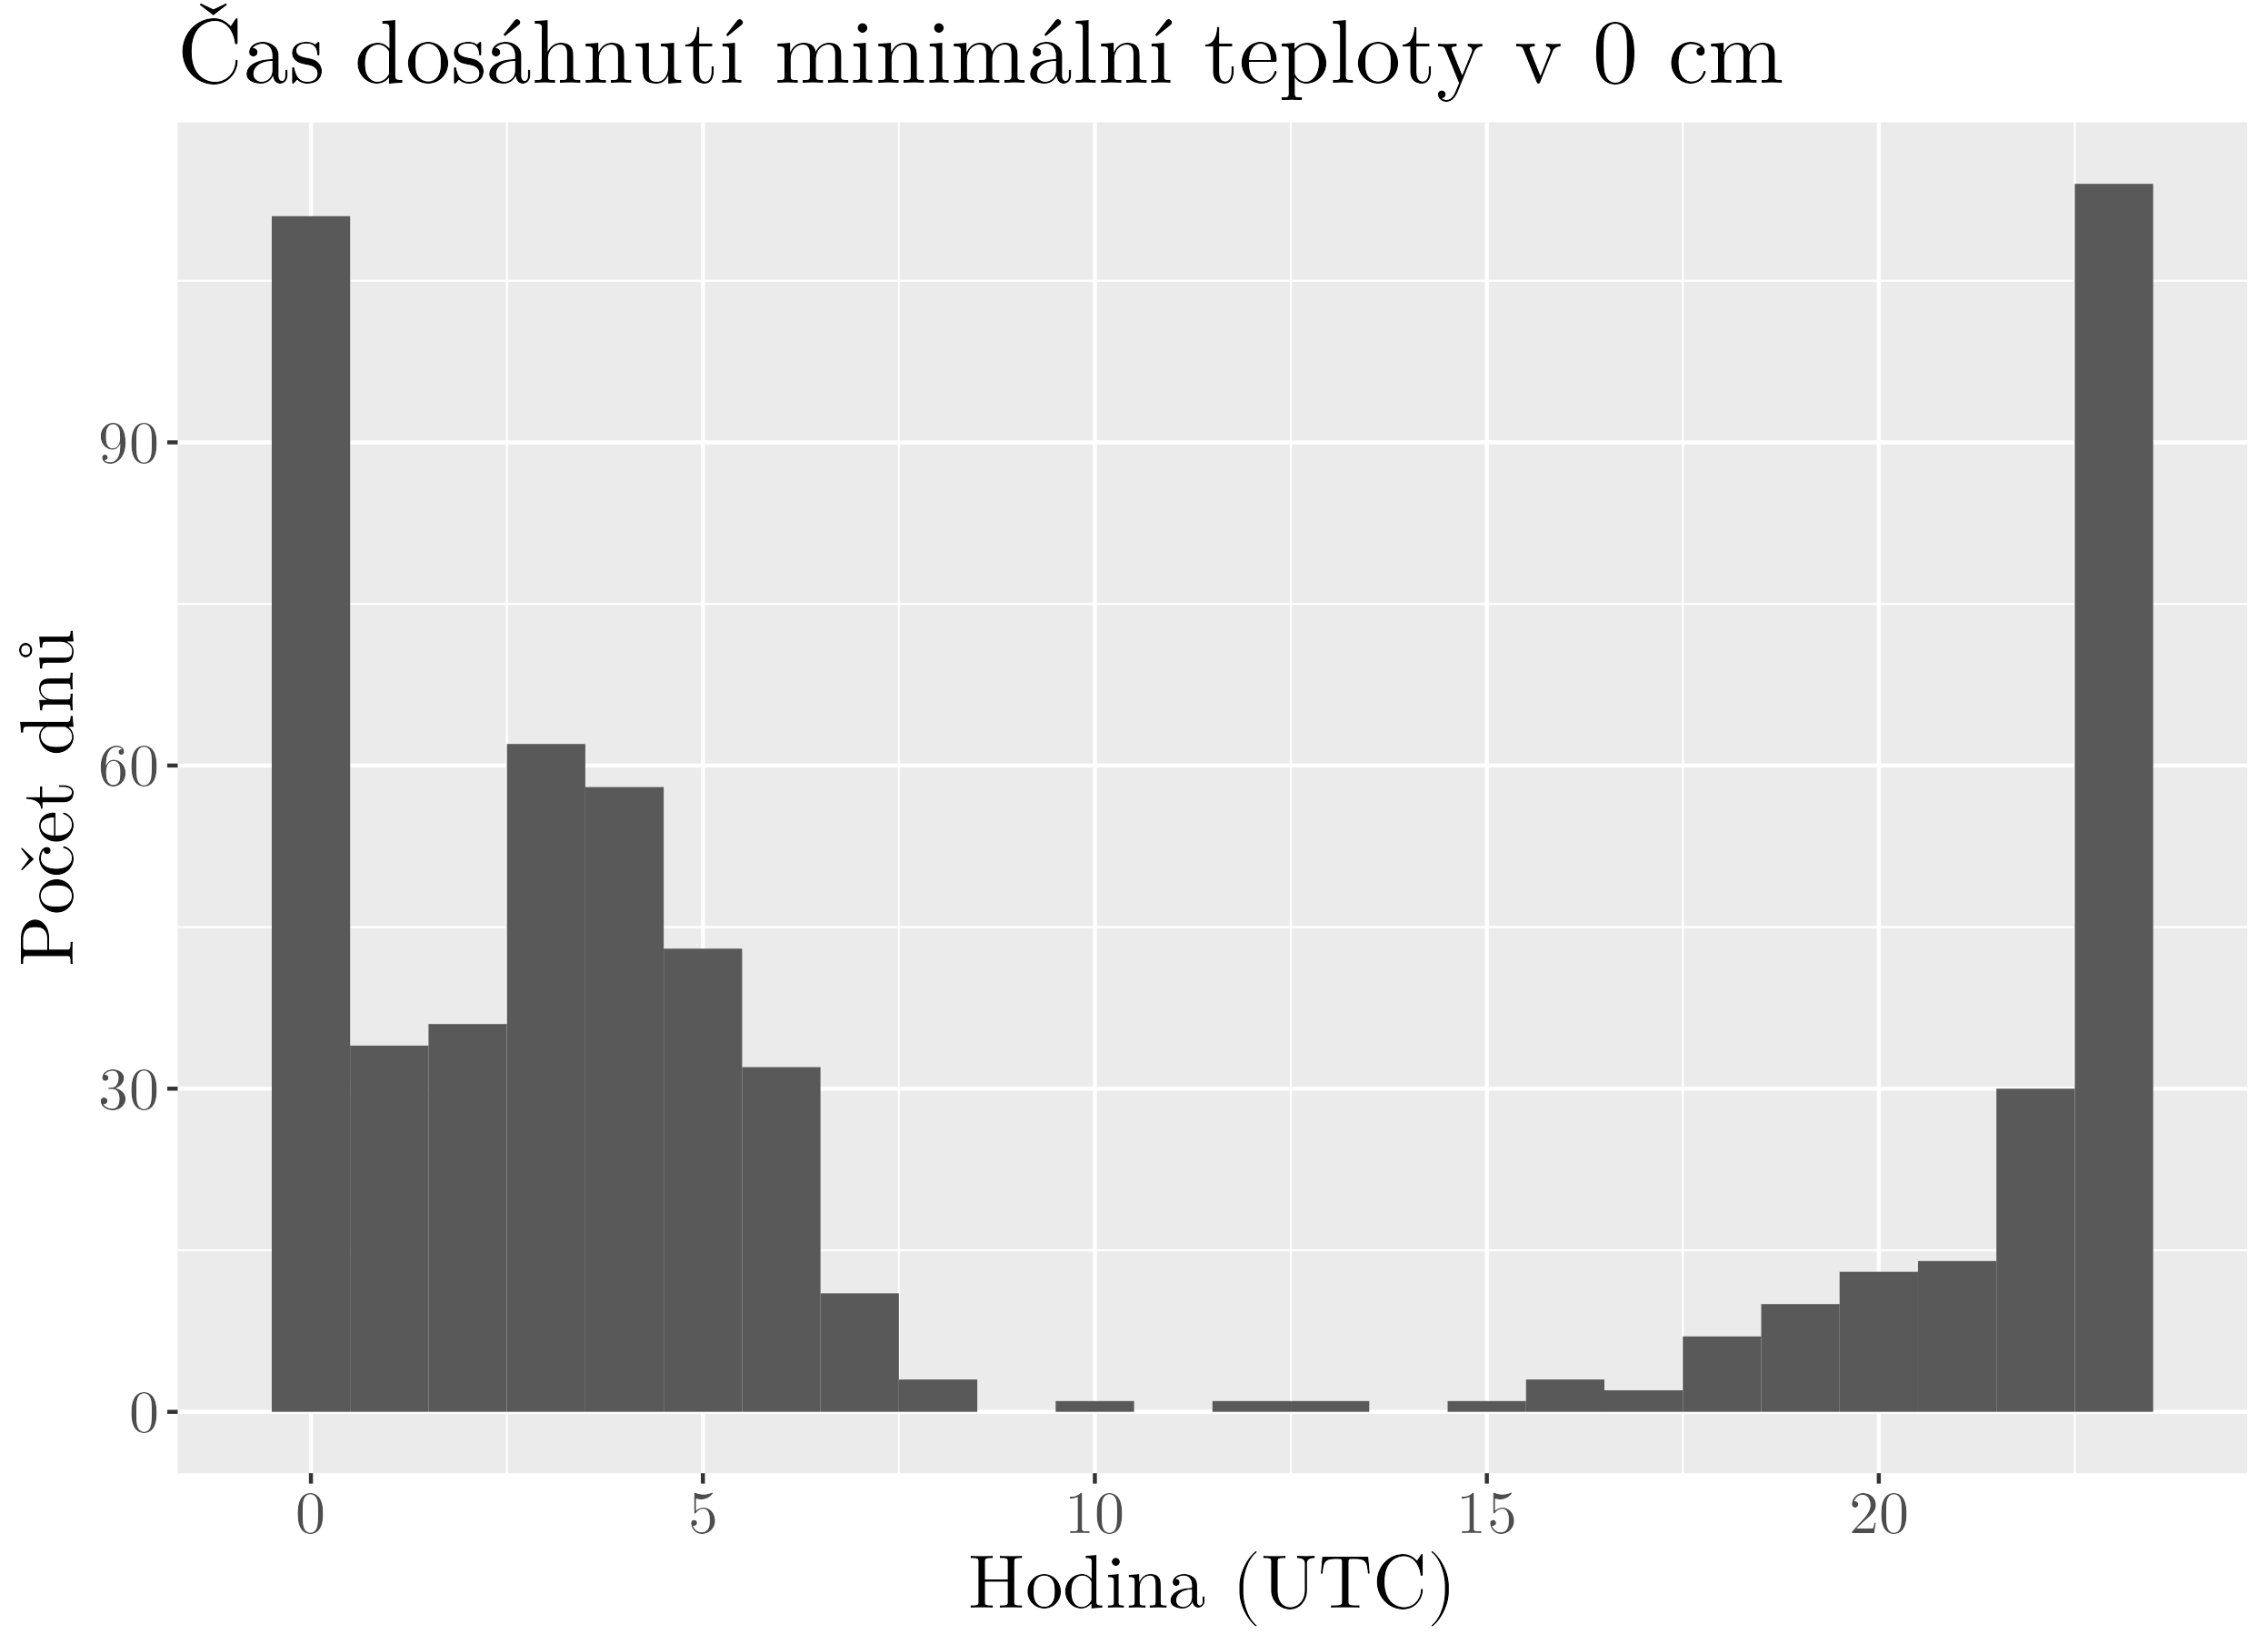
\includegraphics[width=\textwidth]{img/hist_hourmin0cm.png}
		\caption{}
		\label{fig:hourmin0cm}
	\end{subfigure}
	\caption{Denní doba (UTC) dosažení maximální resp. minimální teploty v $\SI{15}{cm}$ resp. v $\SI{0}{cm}$ nad zemí na čidle nejblíže Churáňovu}
	\label{fig:hours}
\end{figure}

Pro ilustraci se ještě podívejme na konkrétní hodnoty teplot pozorované na nejbližším čidlu meteorologické stanice Churáňov. Na obrázcích \ref{fig:maxtemp} můžeme vidět průběh denních minim a maxim na jednom z čidel, celkově jde o období od 12.10.2019 do 20.5.2021 tedy 587 dnů. Na obrázcích \ref{fig:2mhours} můžeme vidět obrázkům \ref{fig:hourmax15cm} a \ref{fig:hourmin15cm} odpovídající hodnoty teplot naměřených ve výšce $\SI{2}{m}$ na čidle zavěšeném na stromě poblíž pozemním čidlům.

\begin{figure}
	\centering
	\begin{subfigure}{0.45\textwidth}
  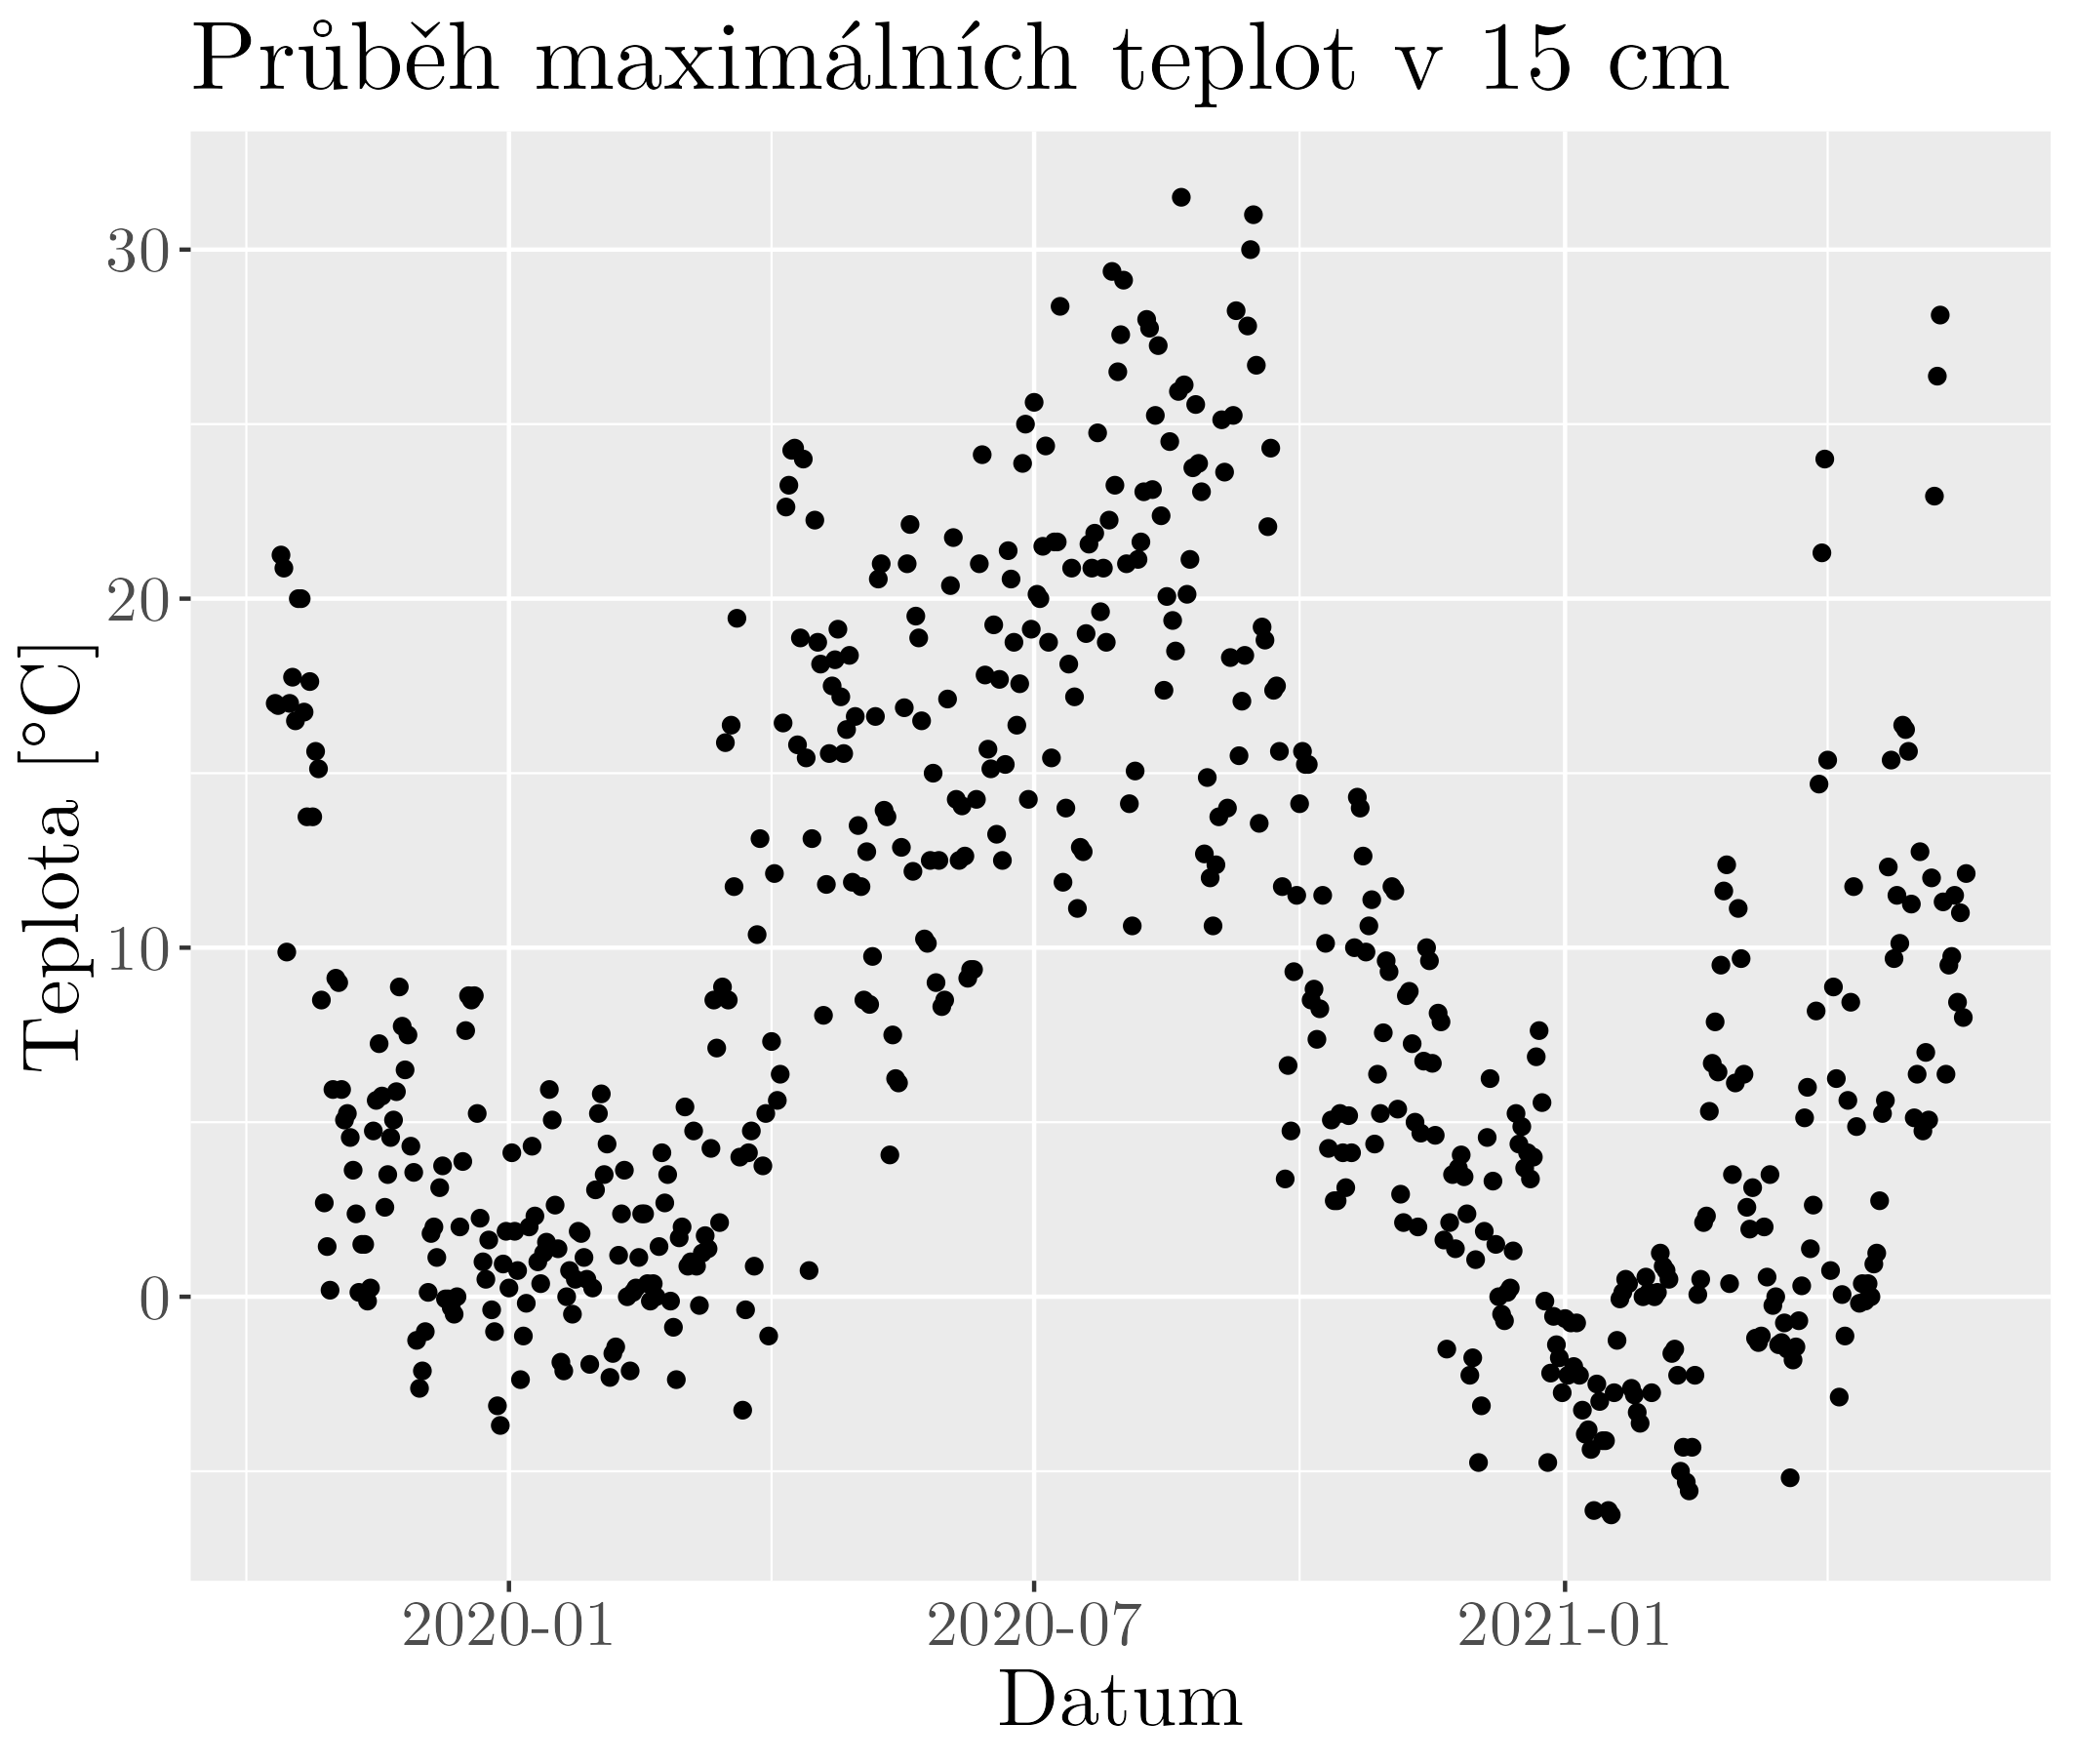
\includegraphics[width=\textwidth]{img/maxtempmax15cm.png}
		\caption{}
		\label{fig:maxtempmax15cm}
	\end{subfigure}
	\hfill
	\begin{subfigure}{0.45\textwidth}
  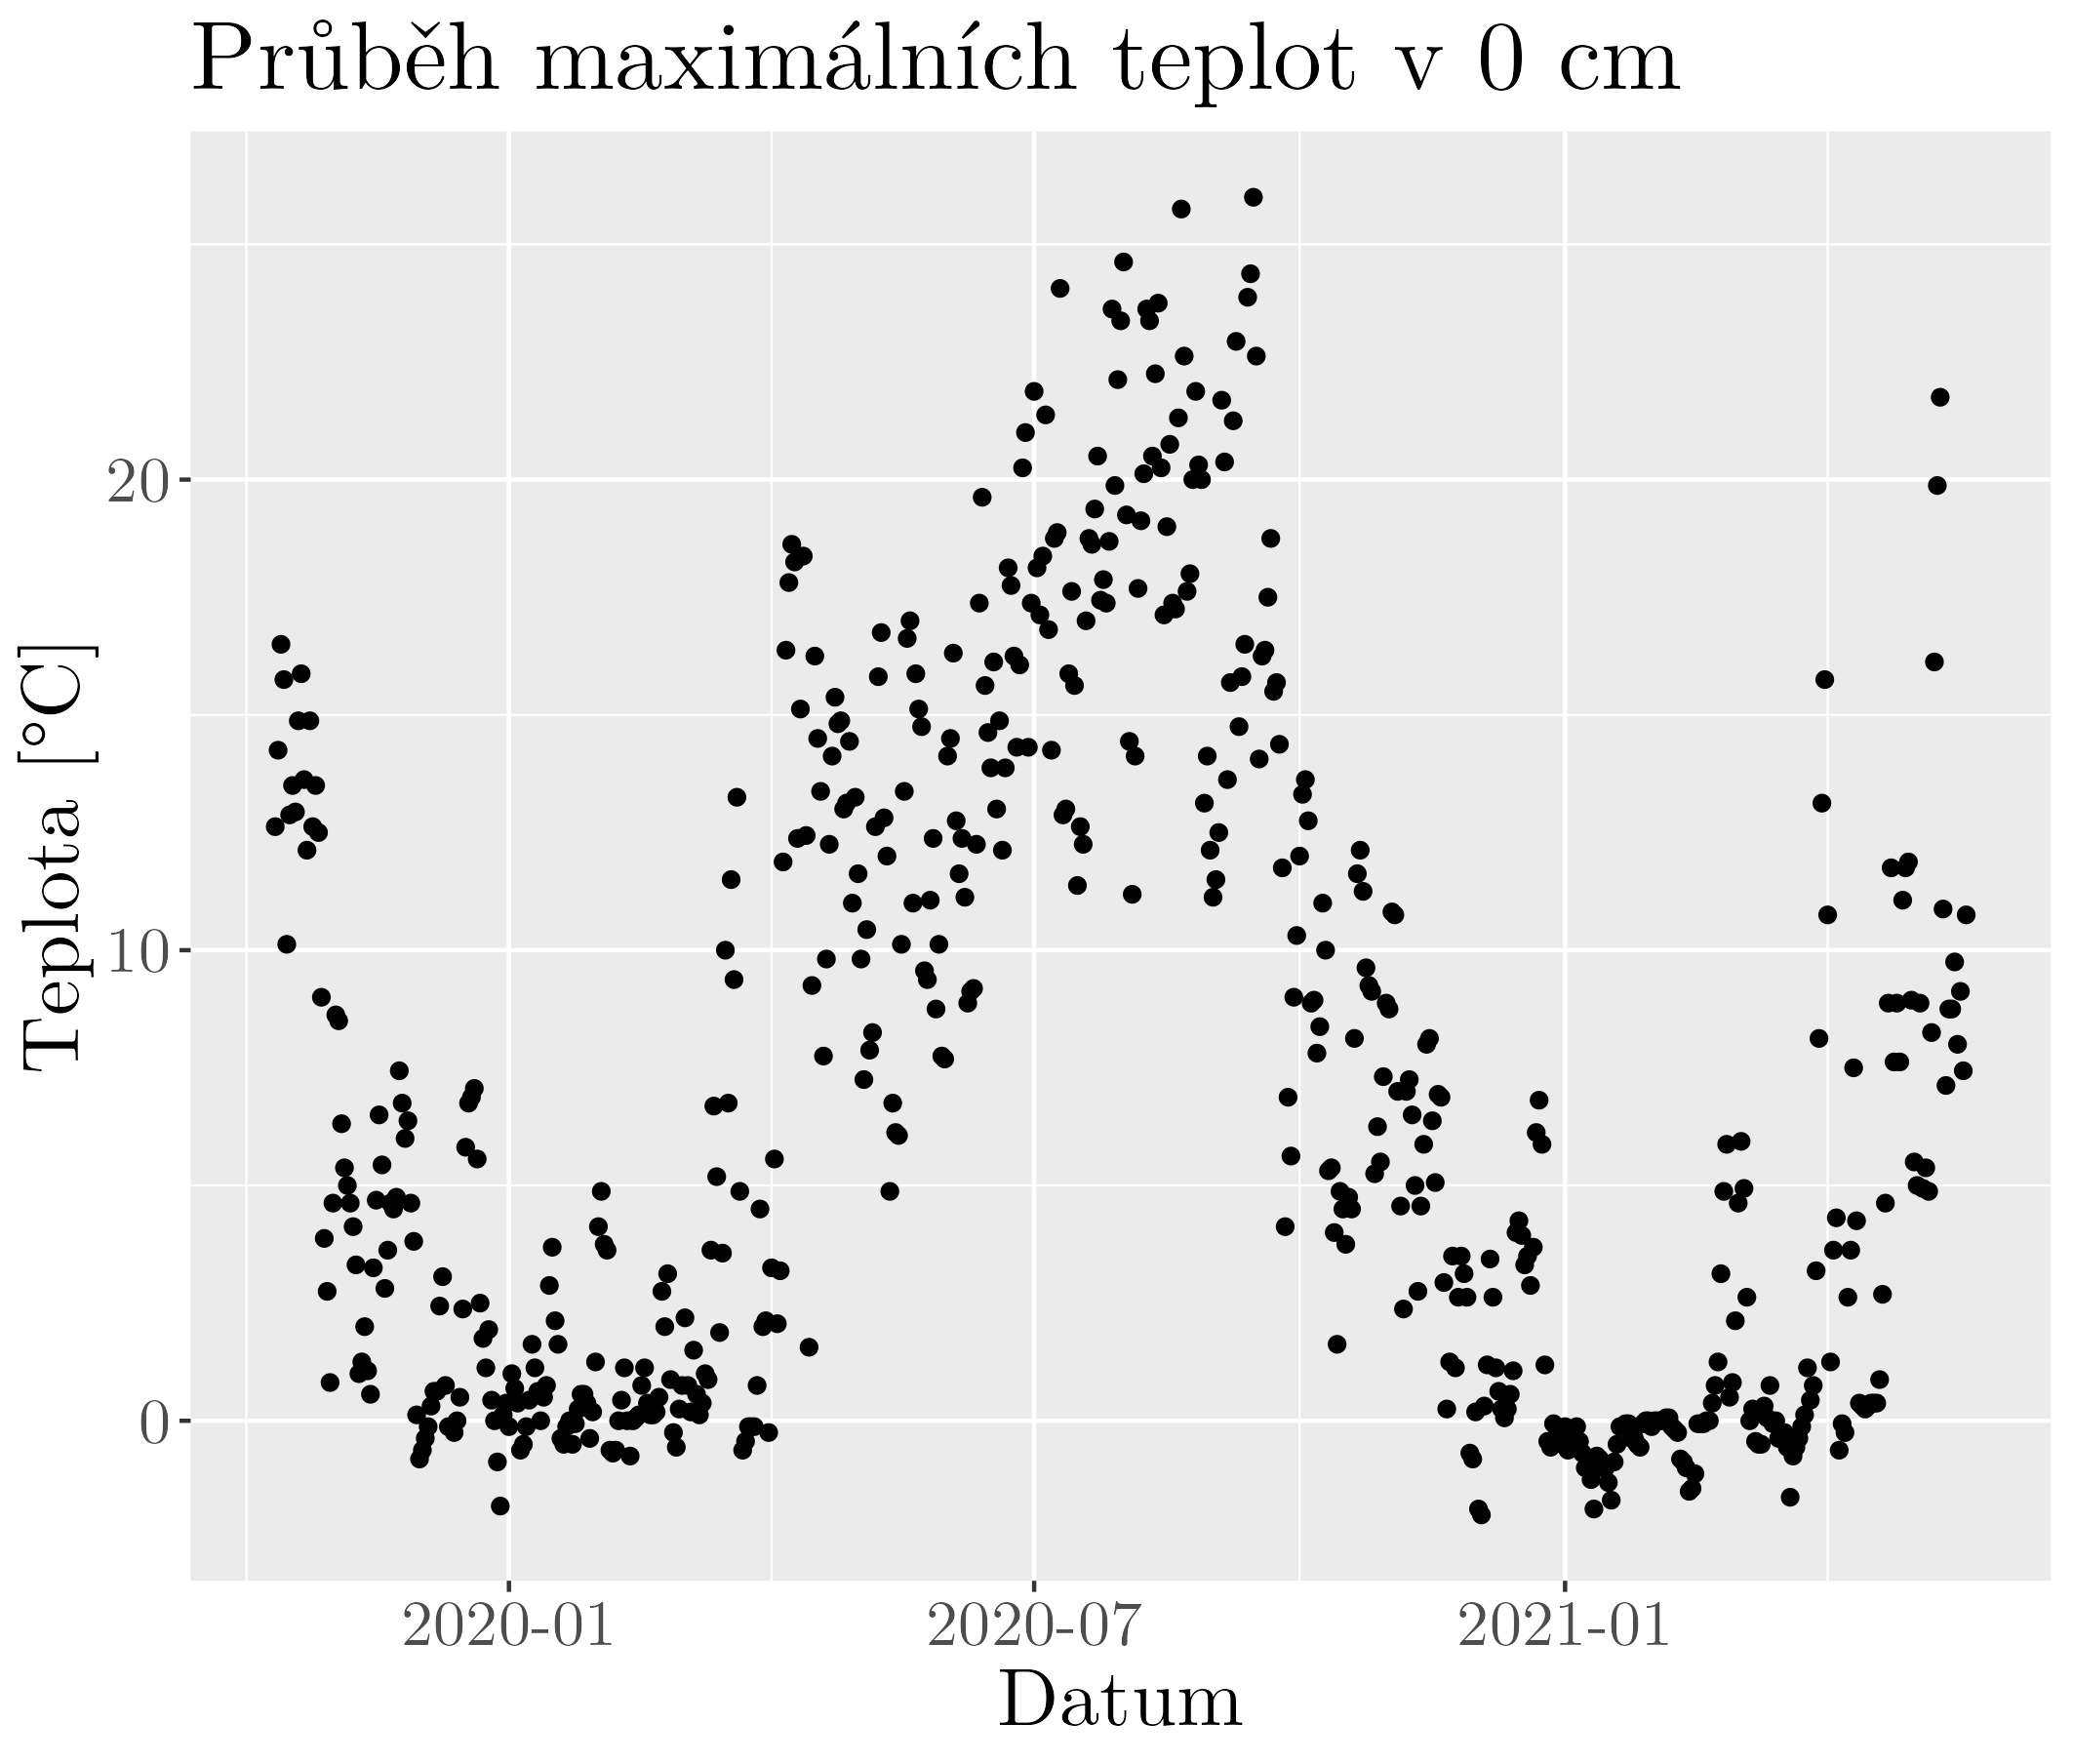
\includegraphics[width=\textwidth]{img/maxtempmax0cm.png}
		\caption{}
		\label{fig:maxtempmax0cm}
	\end{subfigure}
	\hfill
	\begin{subfigure}{0.45\textwidth}
  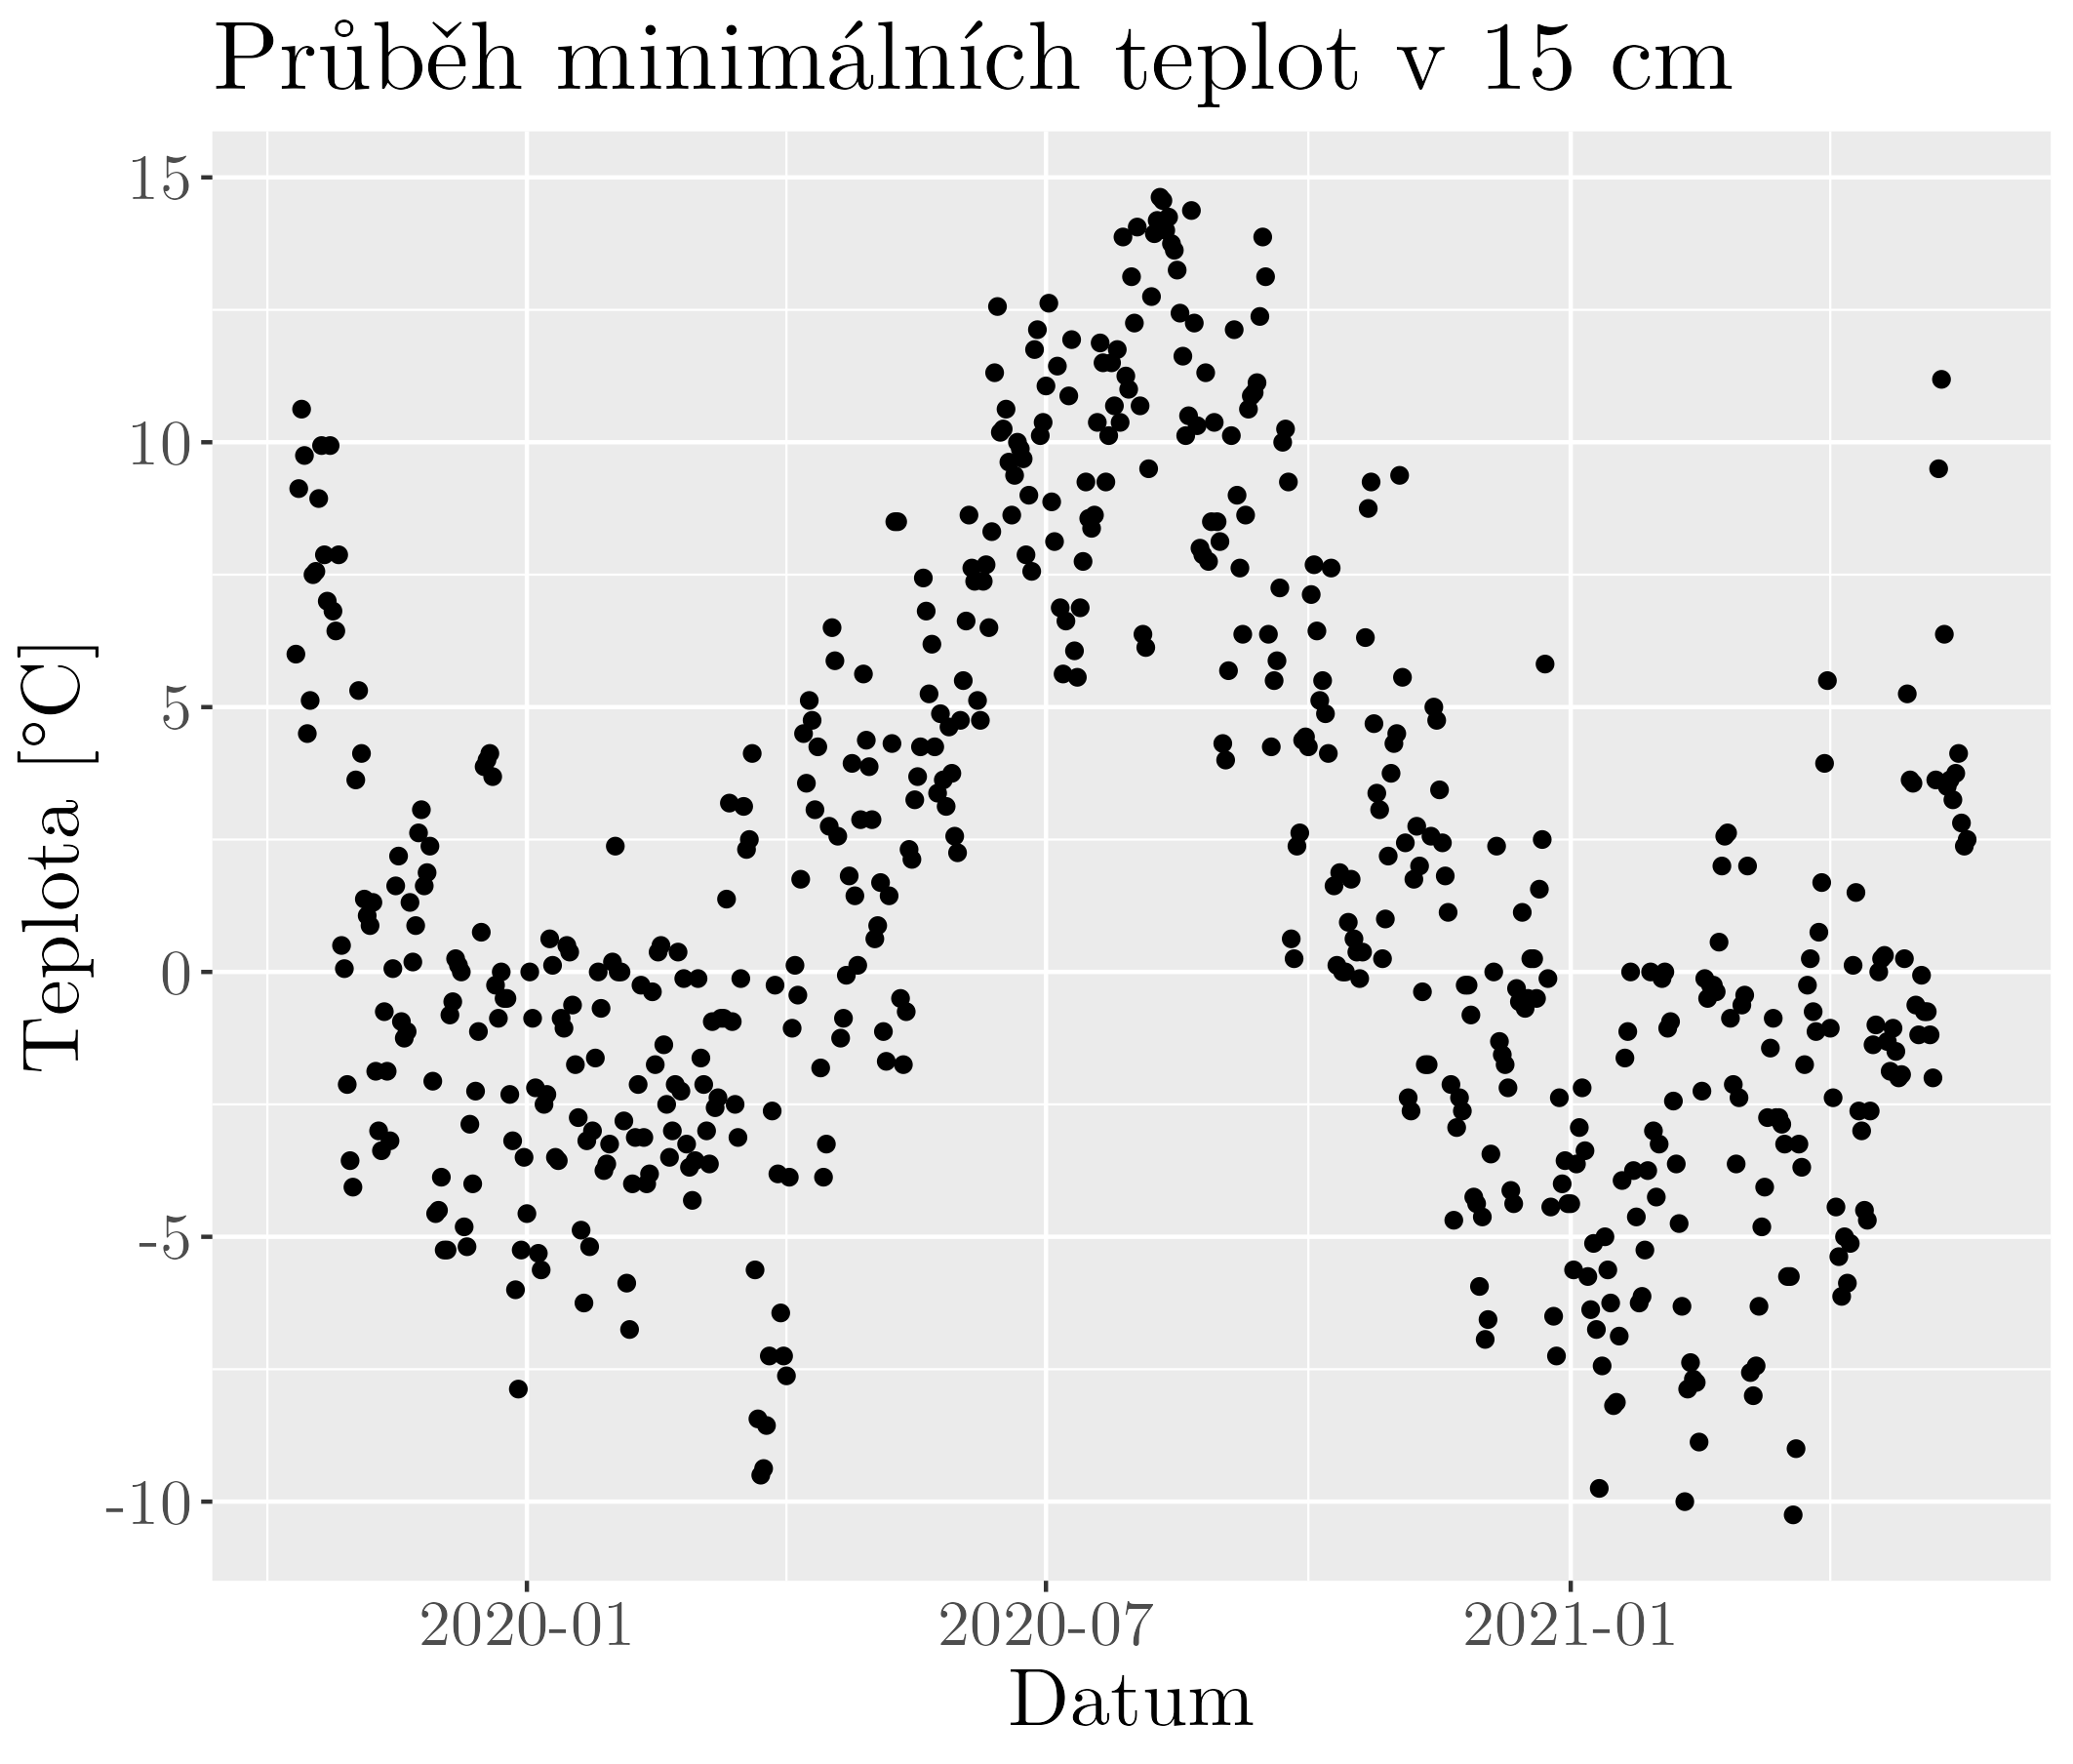
\includegraphics[width=\textwidth]{img/maxtempmin15cm.png}
		\caption{}
		\label{fig:maxtempmin15cm}
	\end{subfigure}
	\hfill
	\begin{subfigure}{0.45\textwidth}
  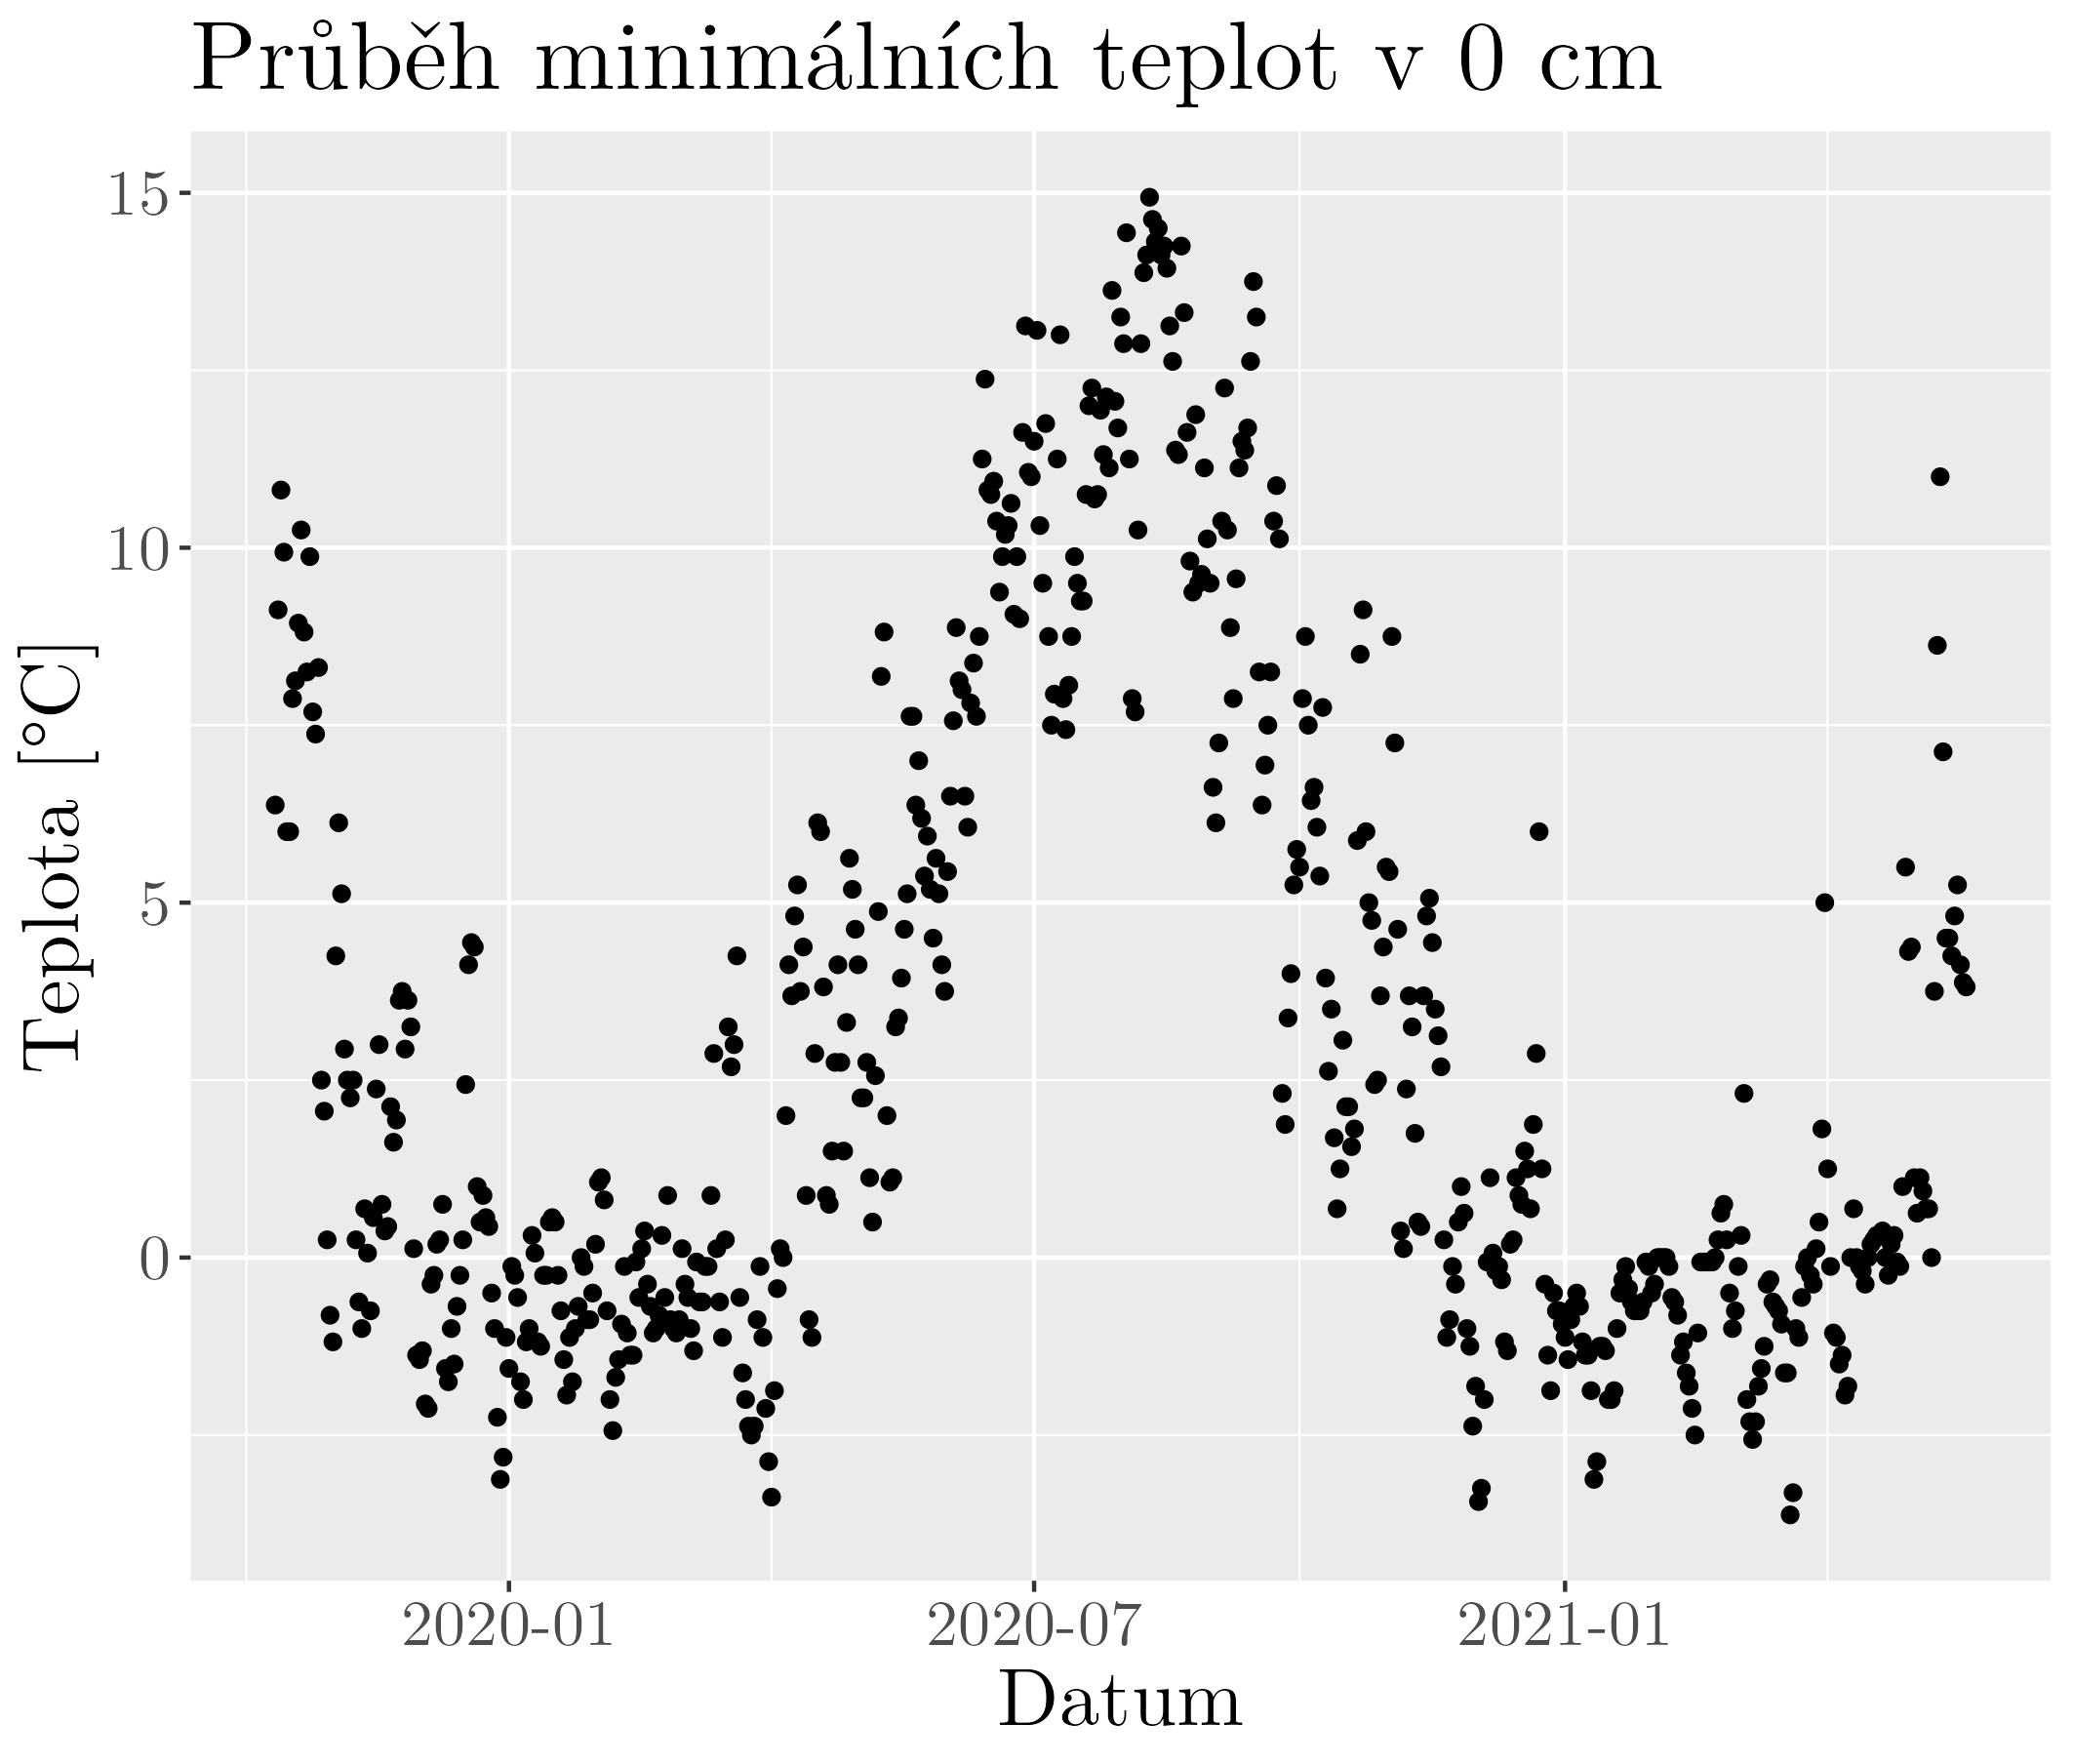
\includegraphics[width=\textwidth]{img/maxtempmin0cm.png}
		\caption{}
		\label{fig:maxtempmin0cm}
	\end{subfigure}
	\caption{Průběh denních maximální resp. minimálních teplot ve výšce $\SI{15}{cm}$ resp. $\SI{0}{cm}$ nad zemí na čidle nejblíže Churáňovu}
	\label{fig:maxtemp}
\end{figure}

\begin{figure}
	\centering
	\begin{subfigure}{0.45\textwidth}
  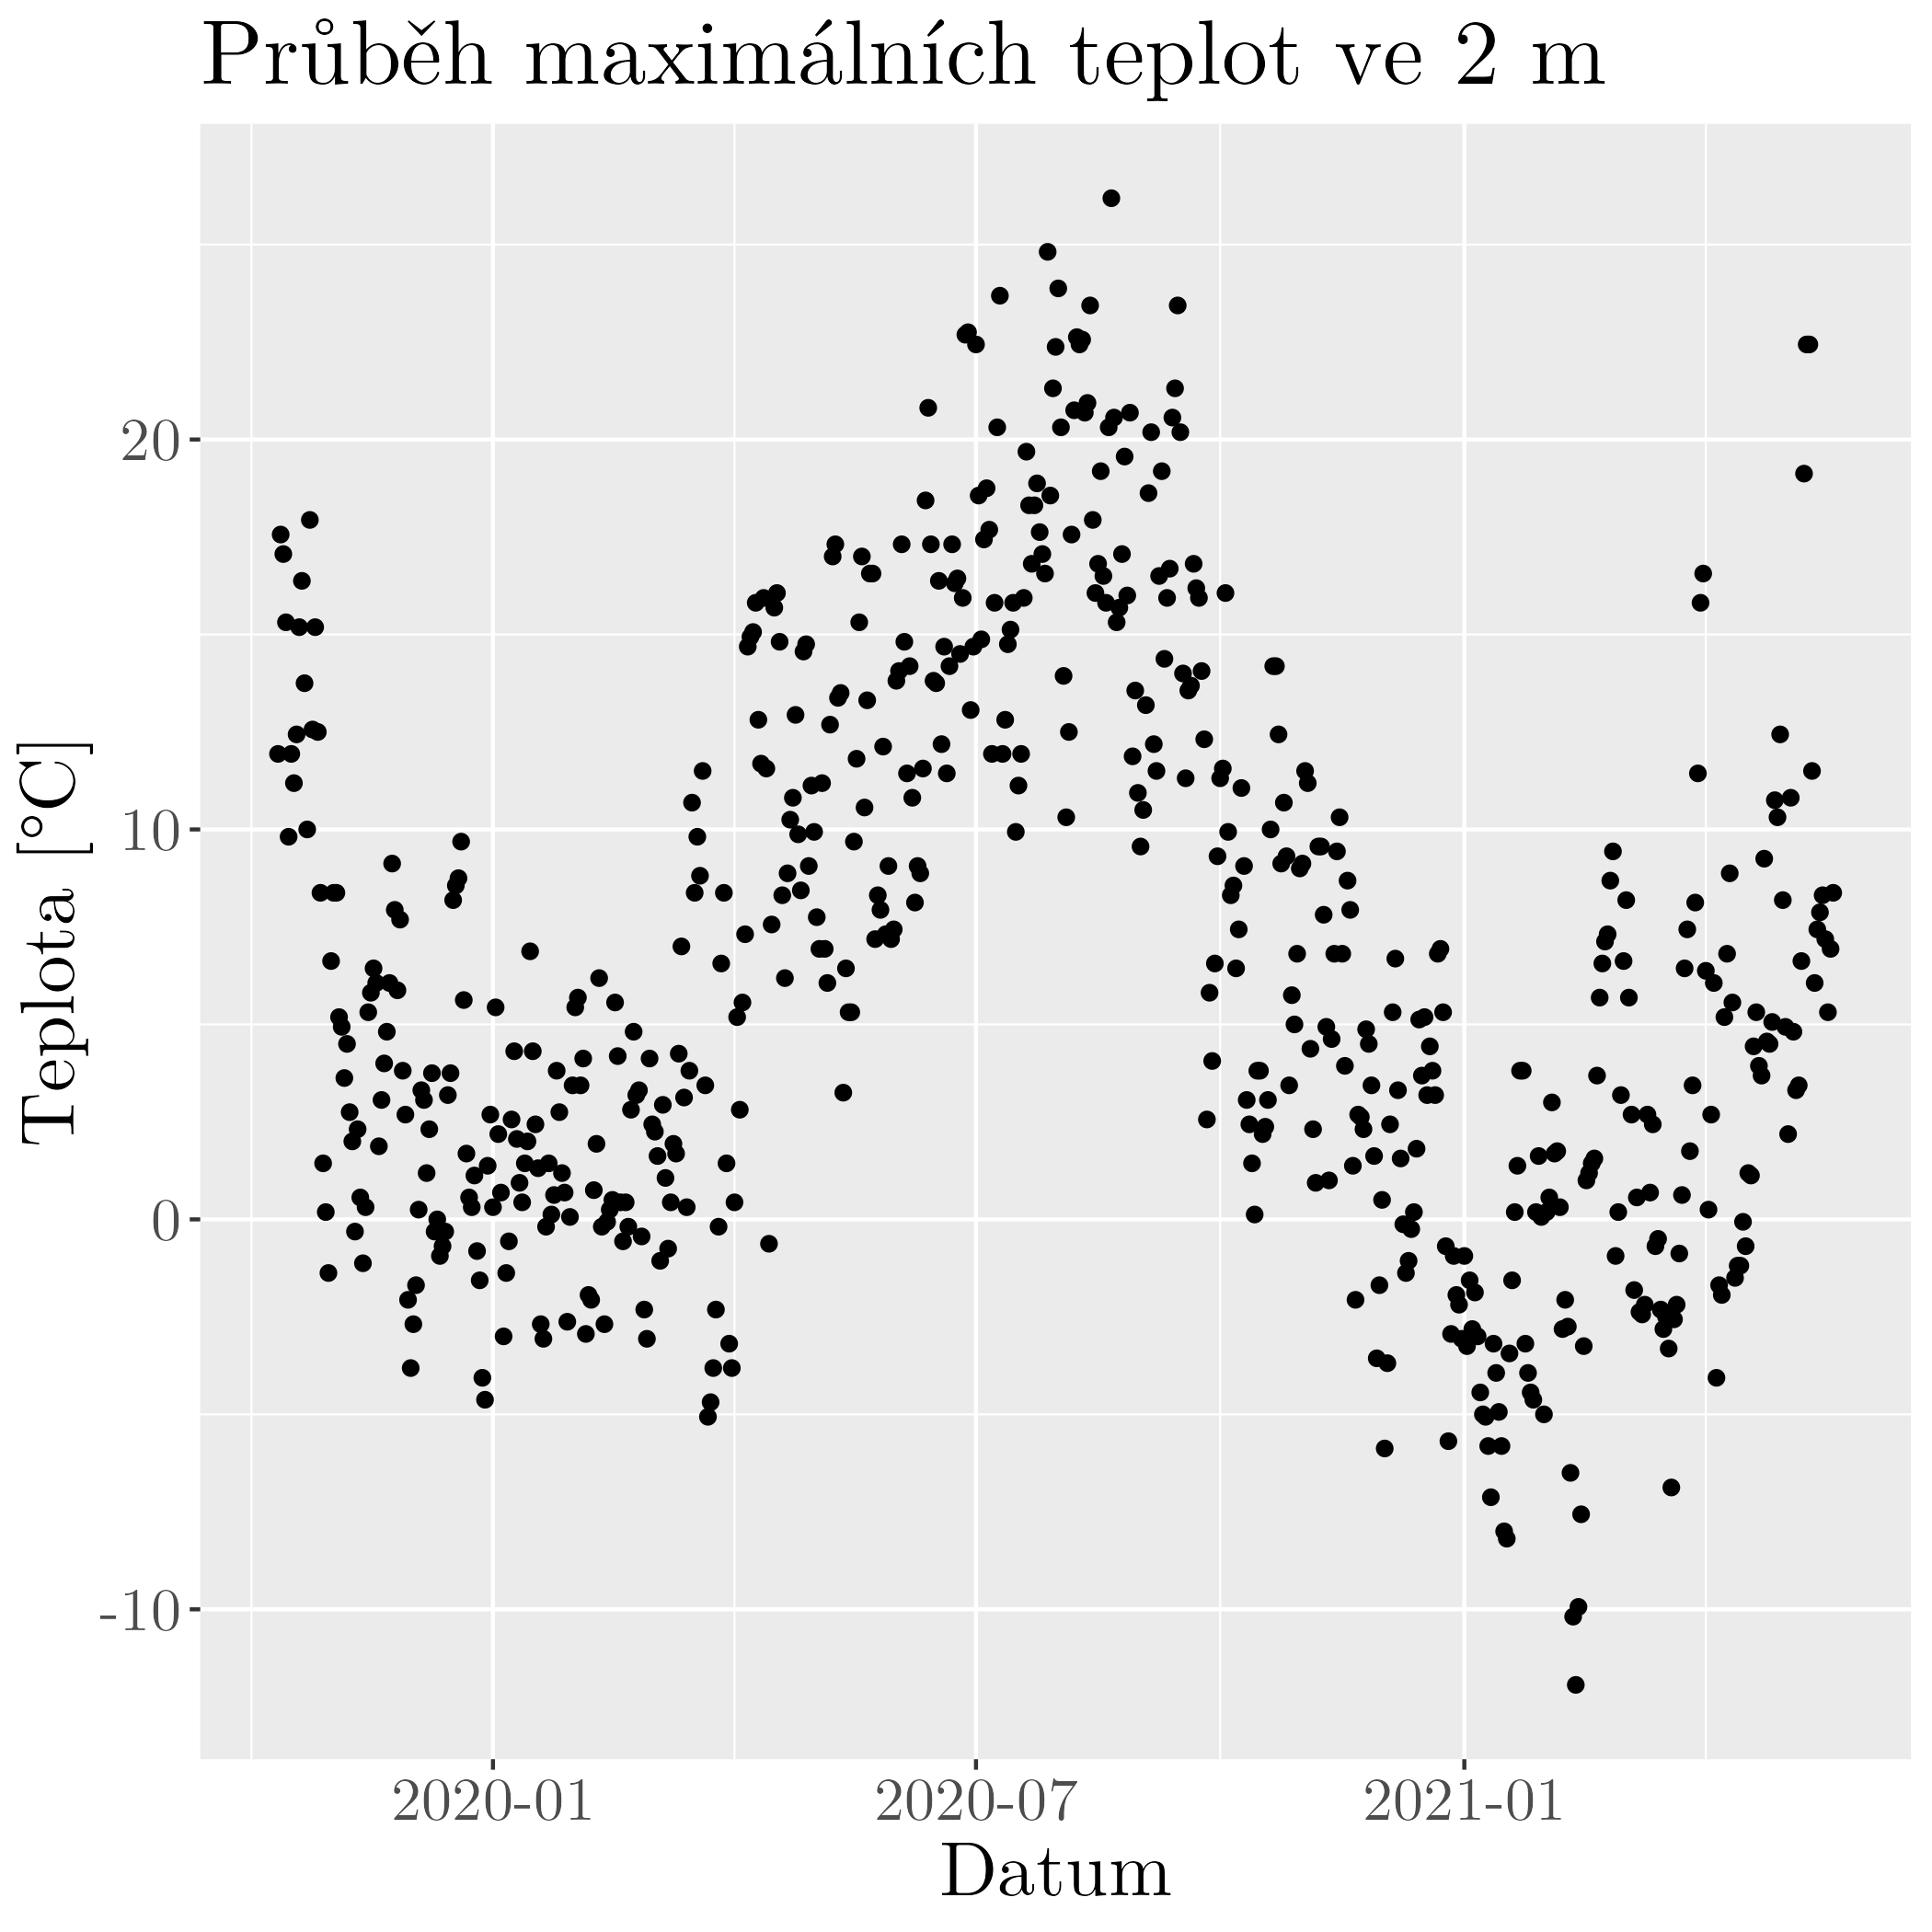
\includegraphics[width=\textwidth]{img/2mmaxtempmax15cm.png}
		\caption{Teploty naměřené ve stejnou dobu jako maximální teploty v $\SI{15}{cm}$}
		\label{fig:2mmaxtempmax15cm}
	\end{subfigure}
	\hfill
	\begin{subfigure}{0.45\textwidth}
  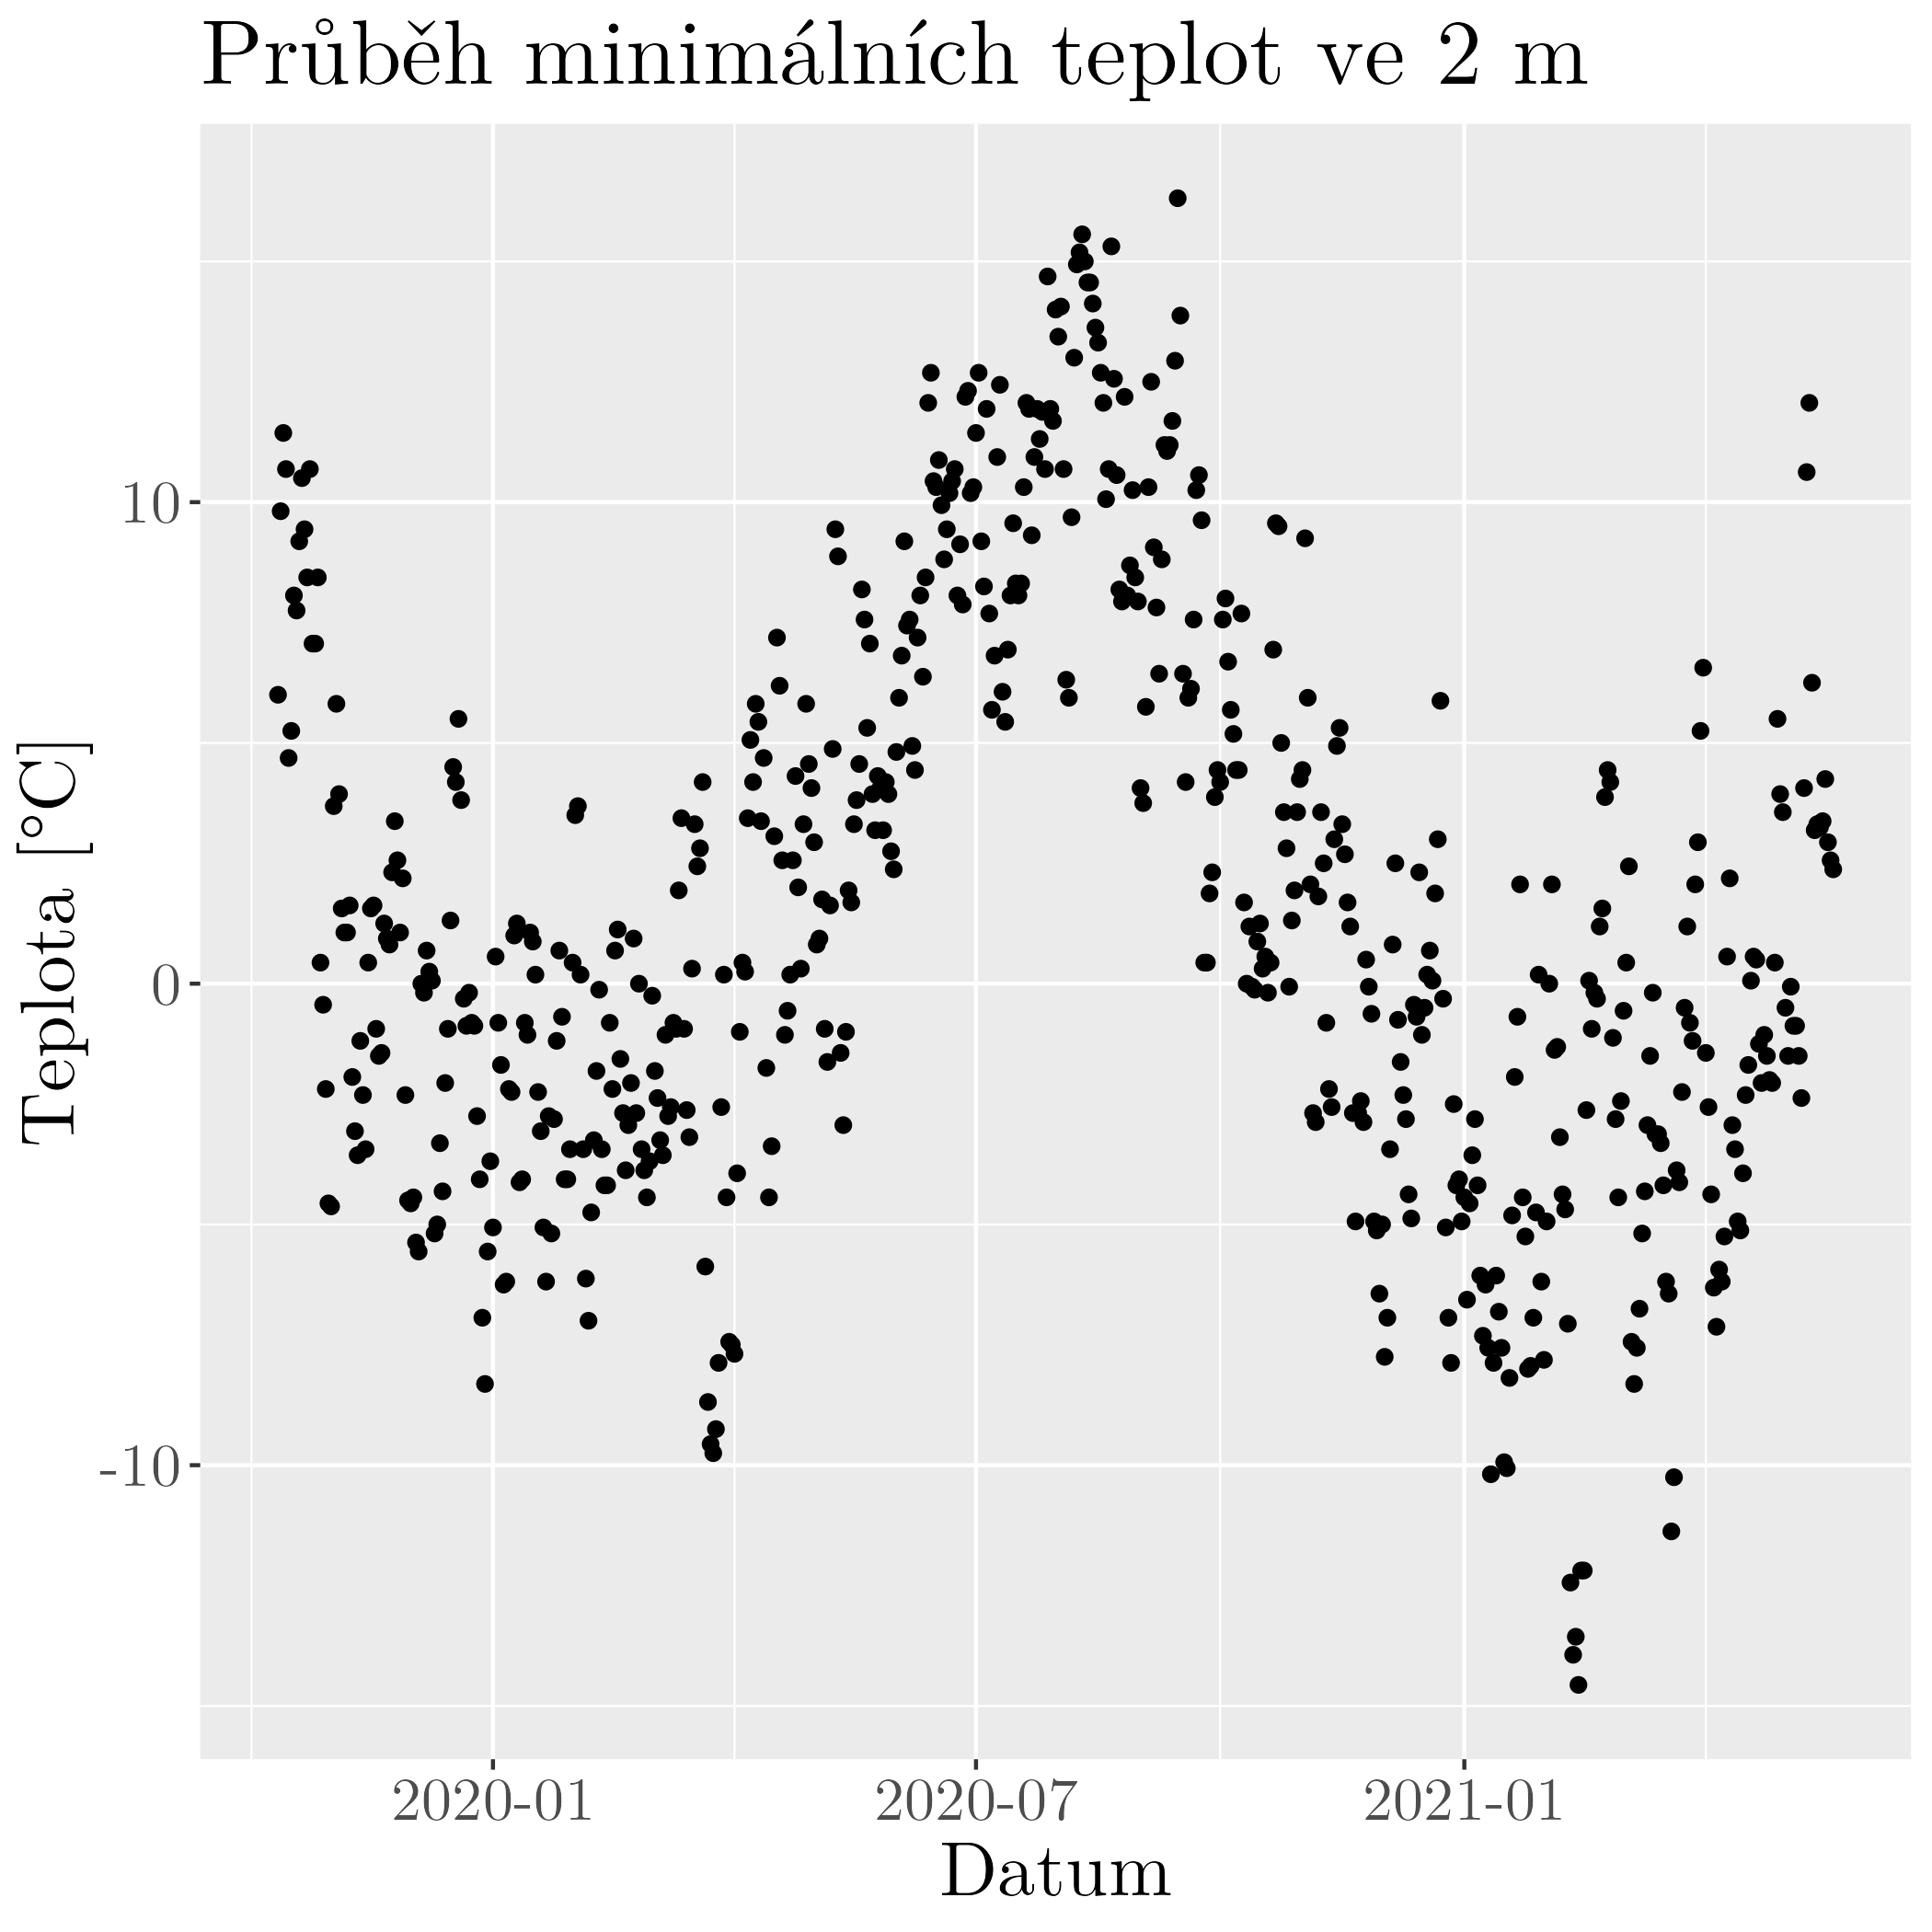
\includegraphics[width=\textwidth]{img/2mmaxtempmin15cm.png}
		\caption{Teploty naměřené ve stejnou dobu jako minimální teploty v $\SI{15}{cm}$}
		\label{fig:2mmaxtempmin15cm}
	\end{subfigure}
	\caption{Teploty ve výšce $\SI{2}{m}$ nad zemí na čidle nejblíže Churáňovu v době kdy nastalo maximum resp. minimum na čidle ve výšce $\SI{15}{cm}$}
	\label{fig:2mhours}
\end{figure}

\section{Metody analýzy dat}
Cílem následující části je ukázat jakým způsobem byly data zpracována, proč byl vybrán daný model a ukázat ověření jeho předpokladů.

\subsection{Autokorelace dat}
Z povahy naměřených dat je zřejmé, že zde bude existovat autokorelace mezi naměřenými maximálními nebo minimálními teplotami. Autokorelace se pak projeví i u rozdílu teploty naměřené blízko země a ve $\SI{2}{m}$. Na obrázku \ref{fig:acf} vidíme autokorelační funkci pro jedno z čidel.

\begin{figure}
	\centering
	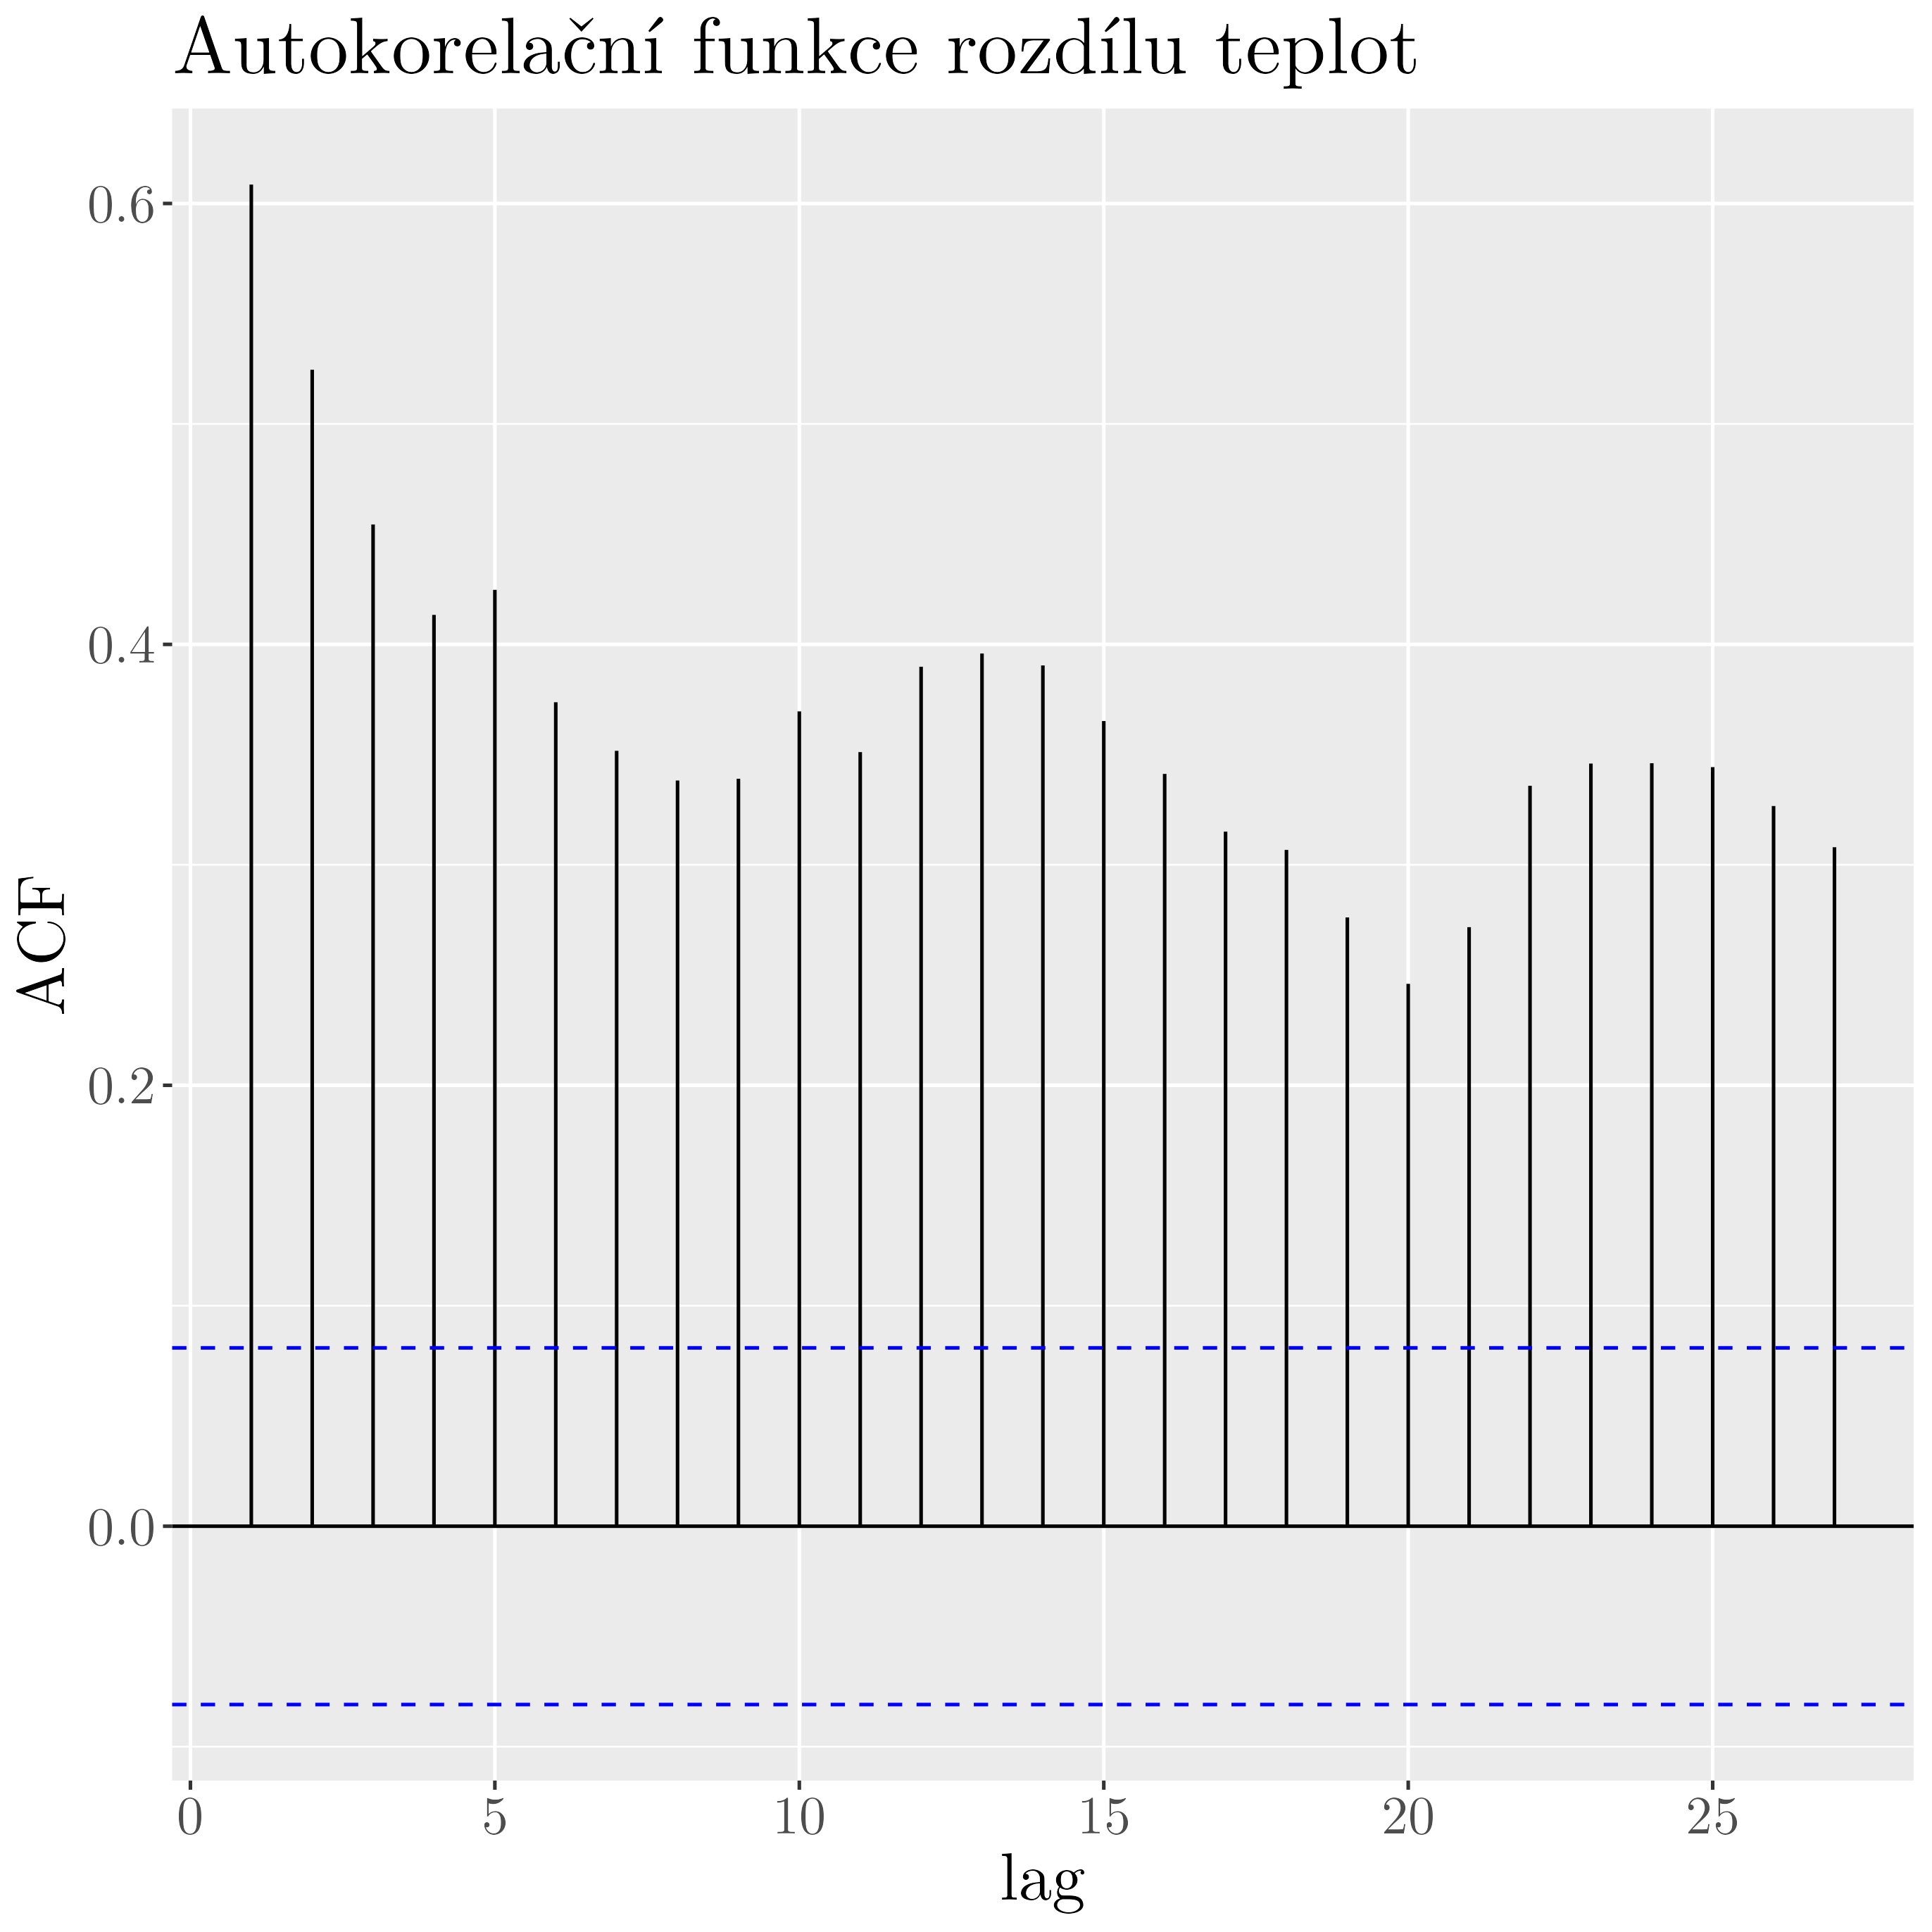
\includegraphics[width=0.55\textwidth]{img/ch2/acfNPS_4311_D_TMS.png}
	\caption{Autokorelační funkce pro rozdíl teplot mezi maximální teplotou v $\SI{15}{cm}$ a teplotou ve $\SI{2}{m}$ na páru čidel nejblíže meteorologické stanici Churáňov.}
	\label{fig:acf}
\end{figure}

Autokorelace není takto významná pro všechna čidla, ale i tak nám vylučuje možnost využít jednoduché mnohonásobné lineární regrese.

\subsection{Lineární model se smíšenými efekty}
Nabízí se využití lineárního modelu se smíšenými efekty. Jako náhodný efekt, jehož reálná hodnota pro nás není důležitá, určíme název čidla. Pro všechna čidla a všechny dostupné dny máme kolem 78000 pozorování rozdílu maximální teploty při zemi a ve $\SI{2}{m}$ (konkrétní počet se může lišit, jestliže bereme teplotu v $\SI{0}{cm}$ nebo $\SI{15}{cm}$ nad zemí). Když vyřadíme měření pro která chybí některá data z meteorologický stanic (typicky oblačnost z Churáňova) a poslední čtyři dny měření, kdy máme data z menšího množství čidel, tak máme 63000 měření.

Zpracovávaná data mají šest prediktorů: insolace, srážky za poslední hodinu, celková sněhová pokrývka, oblačnost, rychlost větru a půdní vlhkost. Oblačnost nabývá fixní hodnot, je vyjádřena v osminách celkové oblačnosti. Rychlost větru je měřená v celočíselných násobcích $\SI{3.6}{m/s}$. Ostatní prediktory, stejně jako rozdíl mezi teplotami při povrchu země který se snažíme vysvětlit, jsou spojité proměnné. 

Pro výpočet lineárního modelu se smíšenými efekty použijeme funkci \texttt{lme} z balíčku \texttt{nlme} programovacího jazyka \texttt{R}.

Pro každý model budeme ověřovat předpoklady, nyní krátce ilustrujeme problémy s kterými se budeme v kapitole \ref{chap:ch3} potýkat na jednom modelu. Pracujeme s maximální denní teplotou ve výšce $\SI{15}{cm}$ a jejím rozdílem od teploty naměřené ve $\SI{2}{m}$. Porovnáme mezi sebou transformace proměnné kterou se snažíme vysvětlit a to bez transformace, s logaritmem, odmocninou a třetí odmocninou. Na obrázcích \ref{fig:qq} vidíme kvantil-kvantilový graf pro jednotlivé transformace. Hodnoty rozdílu teplot jsou ovšem i záporné tudíž místo jednoduchého logaritmu použijeme transformaci \eqref{eq:transformace}. Podobně ošetříme záporné hodnoty i pro ostatní transformace.

\begin{gather*}
T \mapsto \mathrm{sign}(T)\cdot \ln\left|T\right| \label{eq:transformace}
\end{gather*}

\begin{figure}
	\centering
	\begin{subfigure}{0.45\textwidth}
  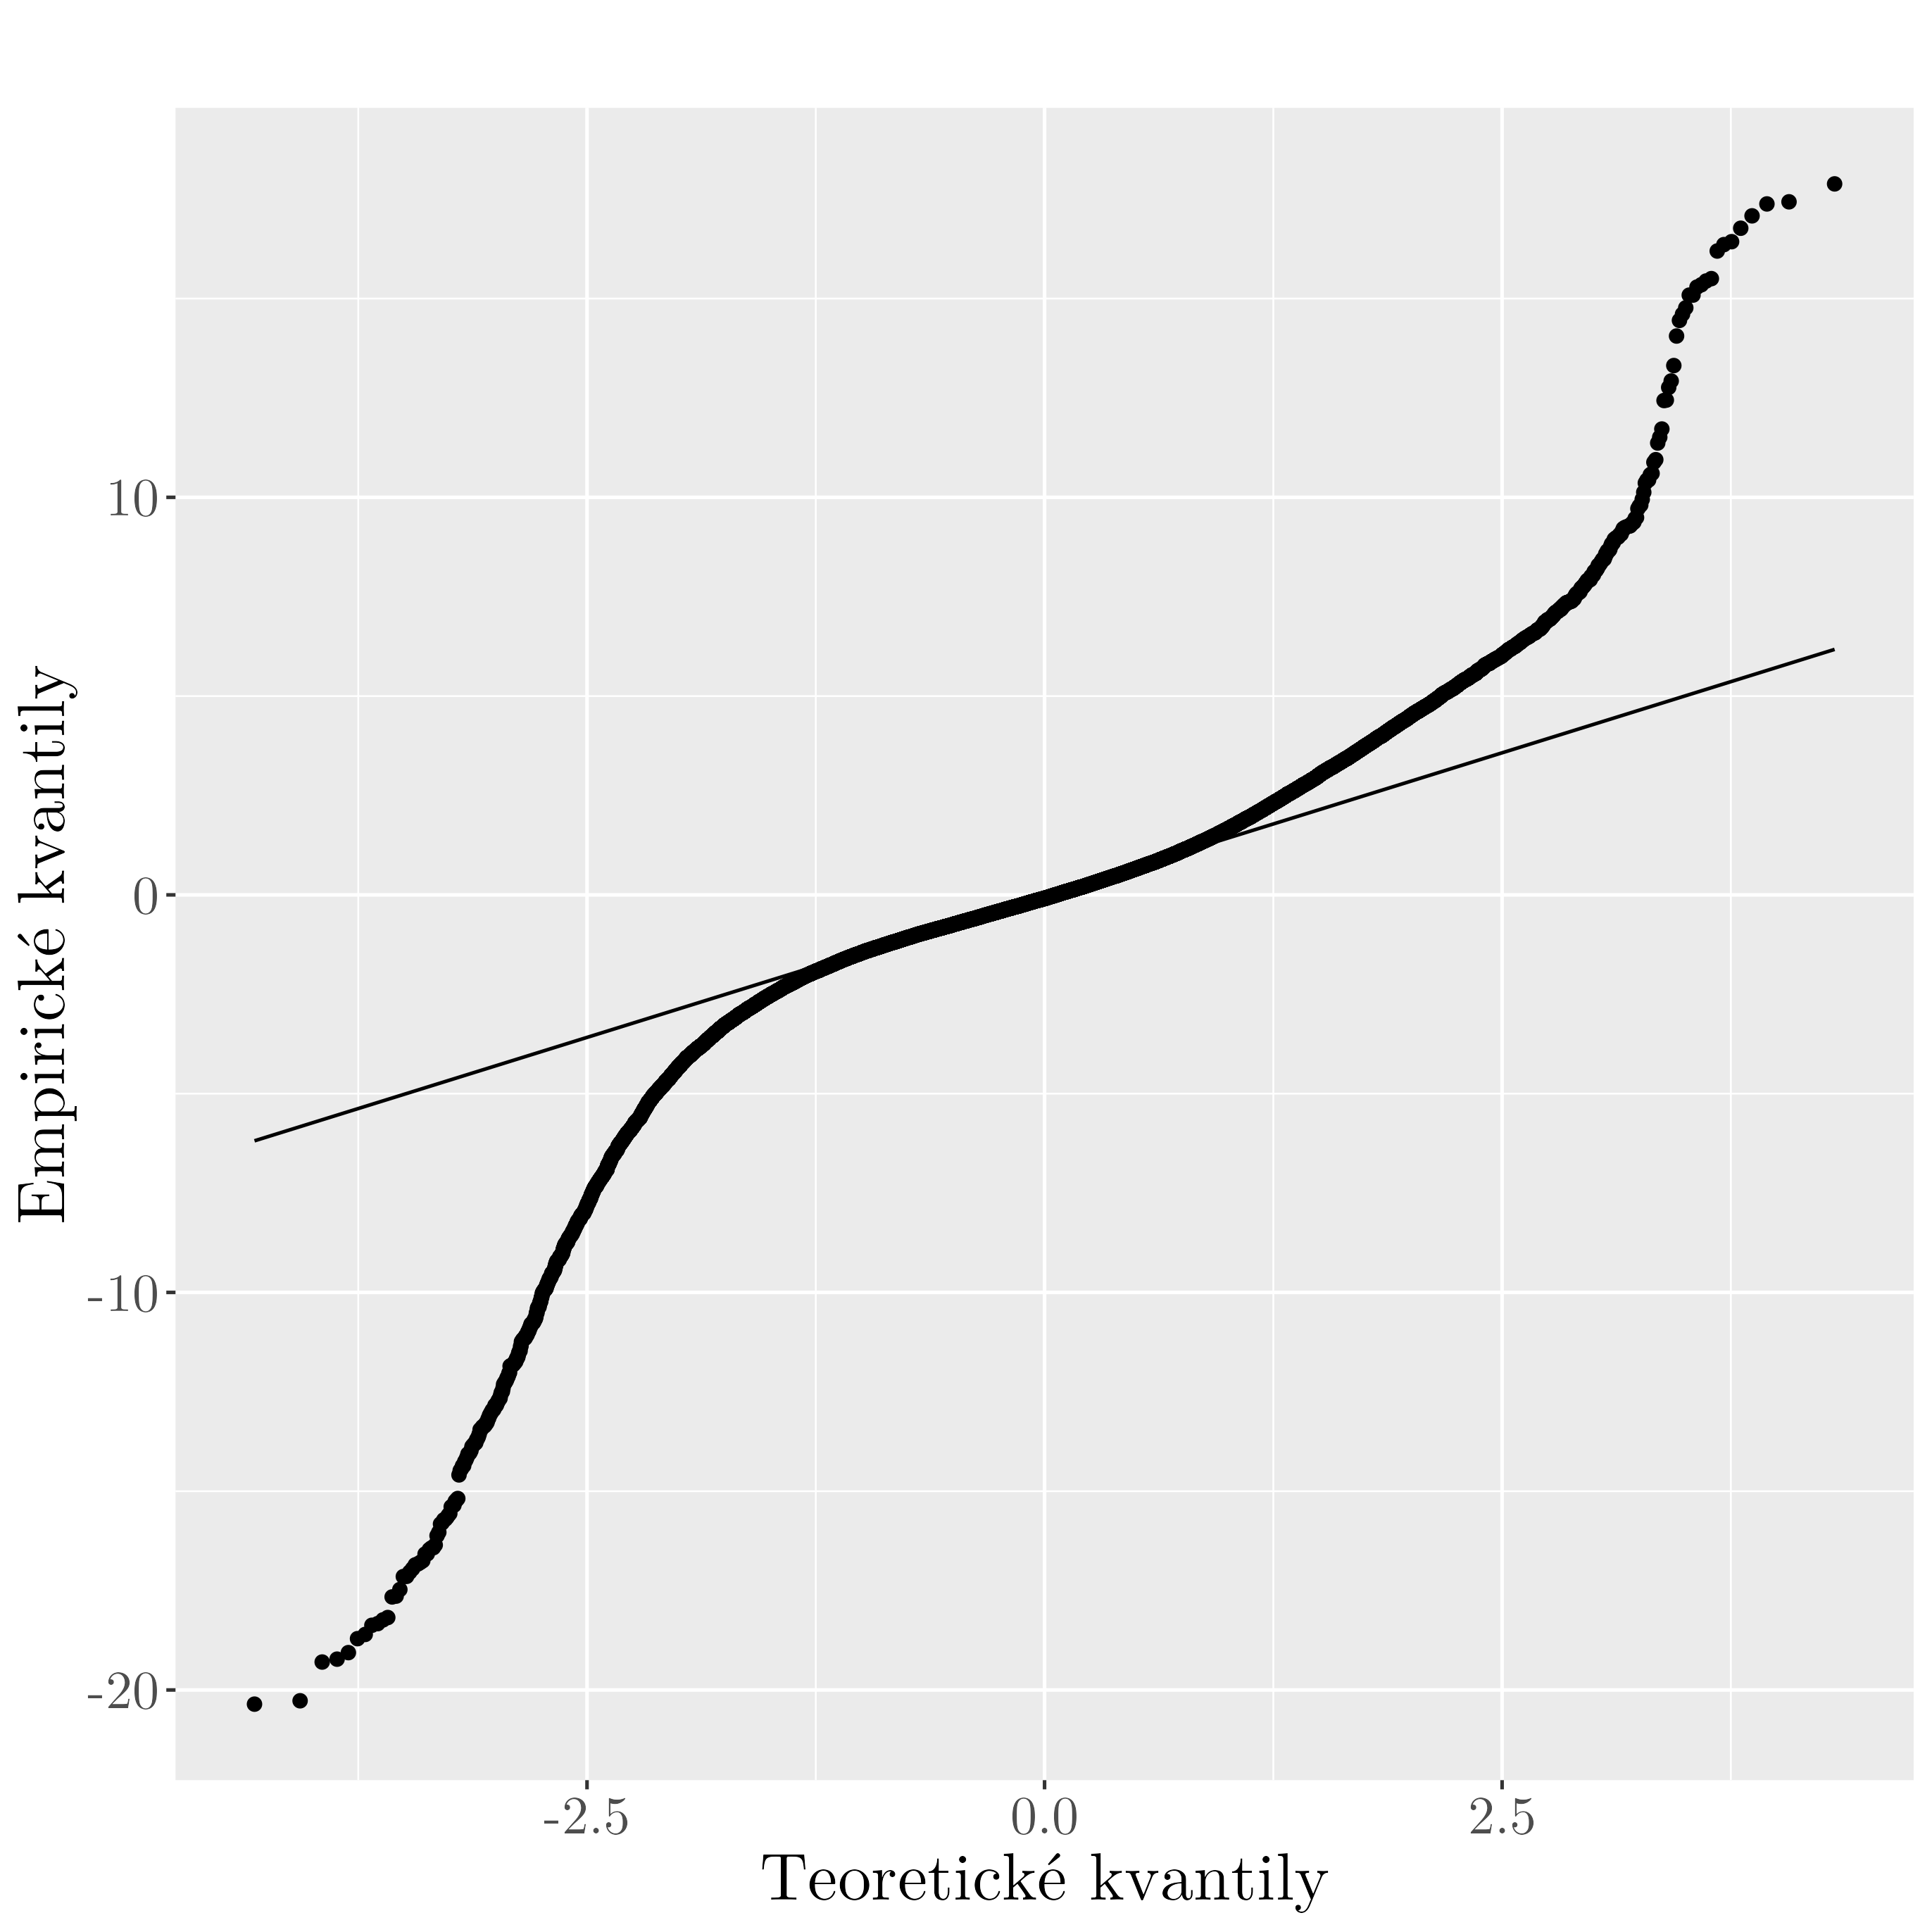
\includegraphics[width=\textwidth]{img/ch2/qq_modmax15cm_none.png}
		\caption{Bez transformace}
		\label{fig:qq_none}
	\end{subfigure}
	\hfill
	\begin{subfigure}{0.45\textwidth}
  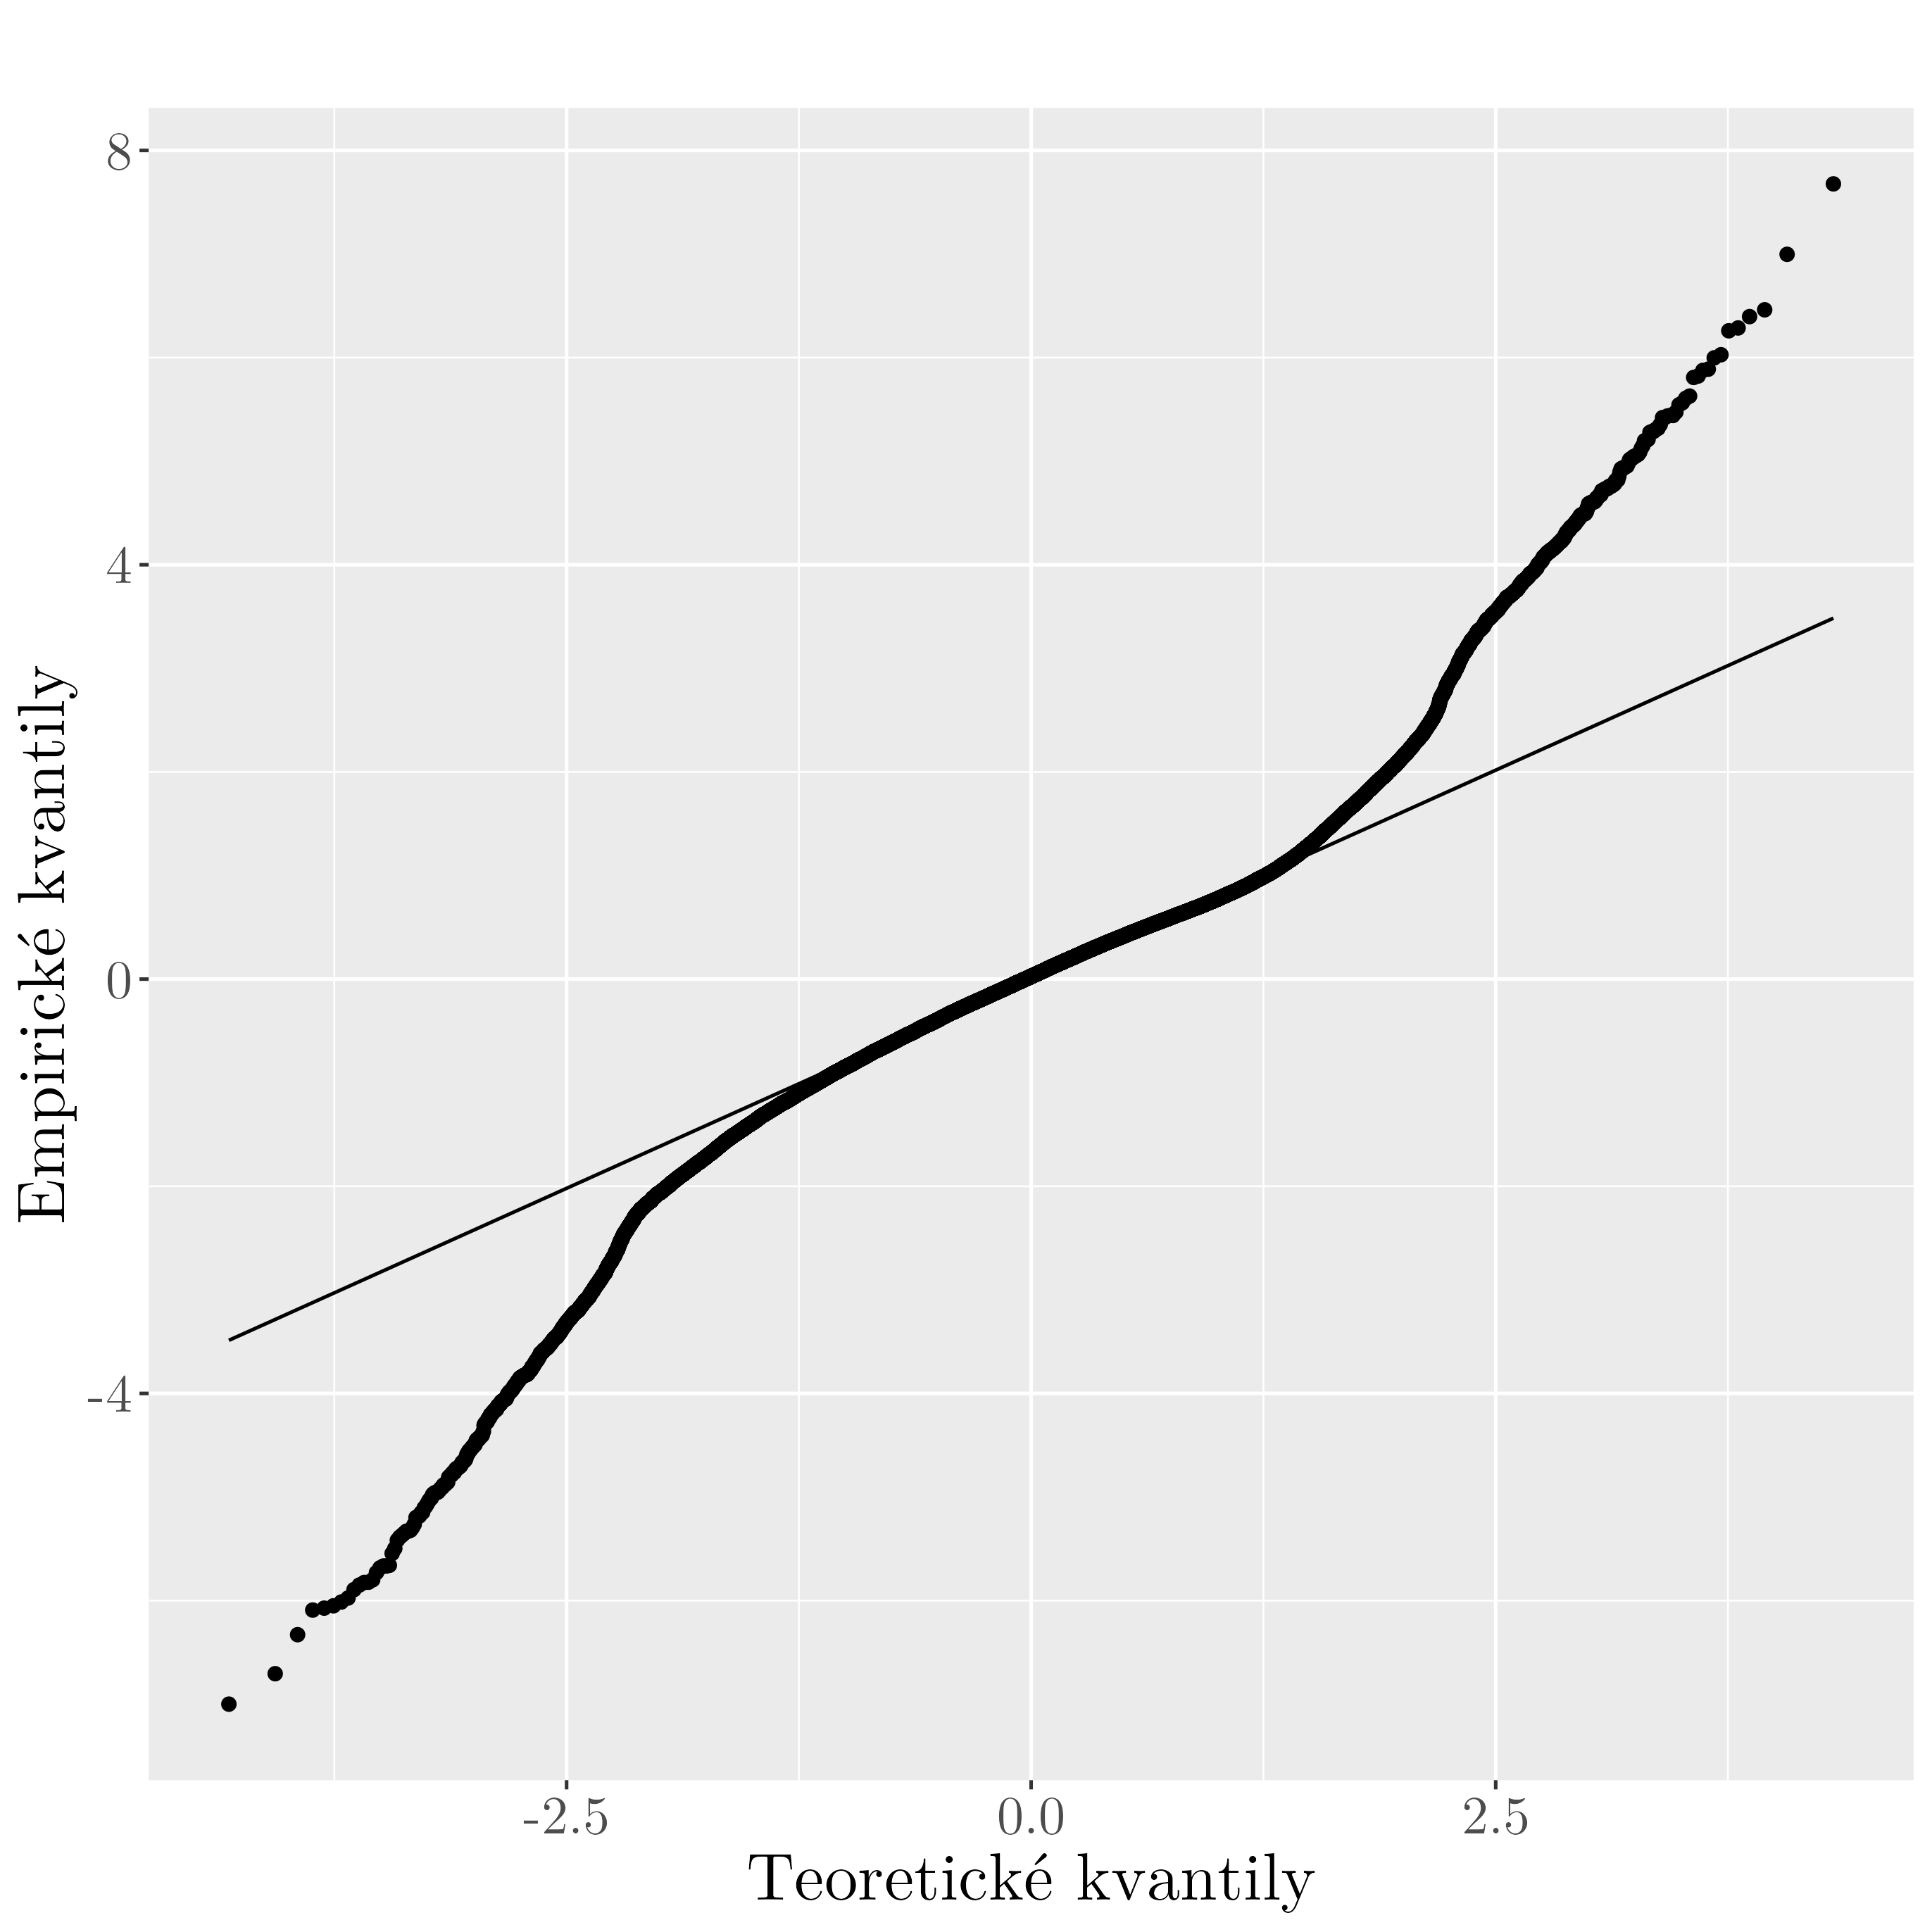
\includegraphics[width=\textwidth]{img/ch2/qq_modmax15cm_log.png}
		\caption{Přirozený logaritmus}
		\label{fig:qq_log}
	\end{subfigure}
	\hfill
	\begin{subfigure}{0.45\textwidth}
  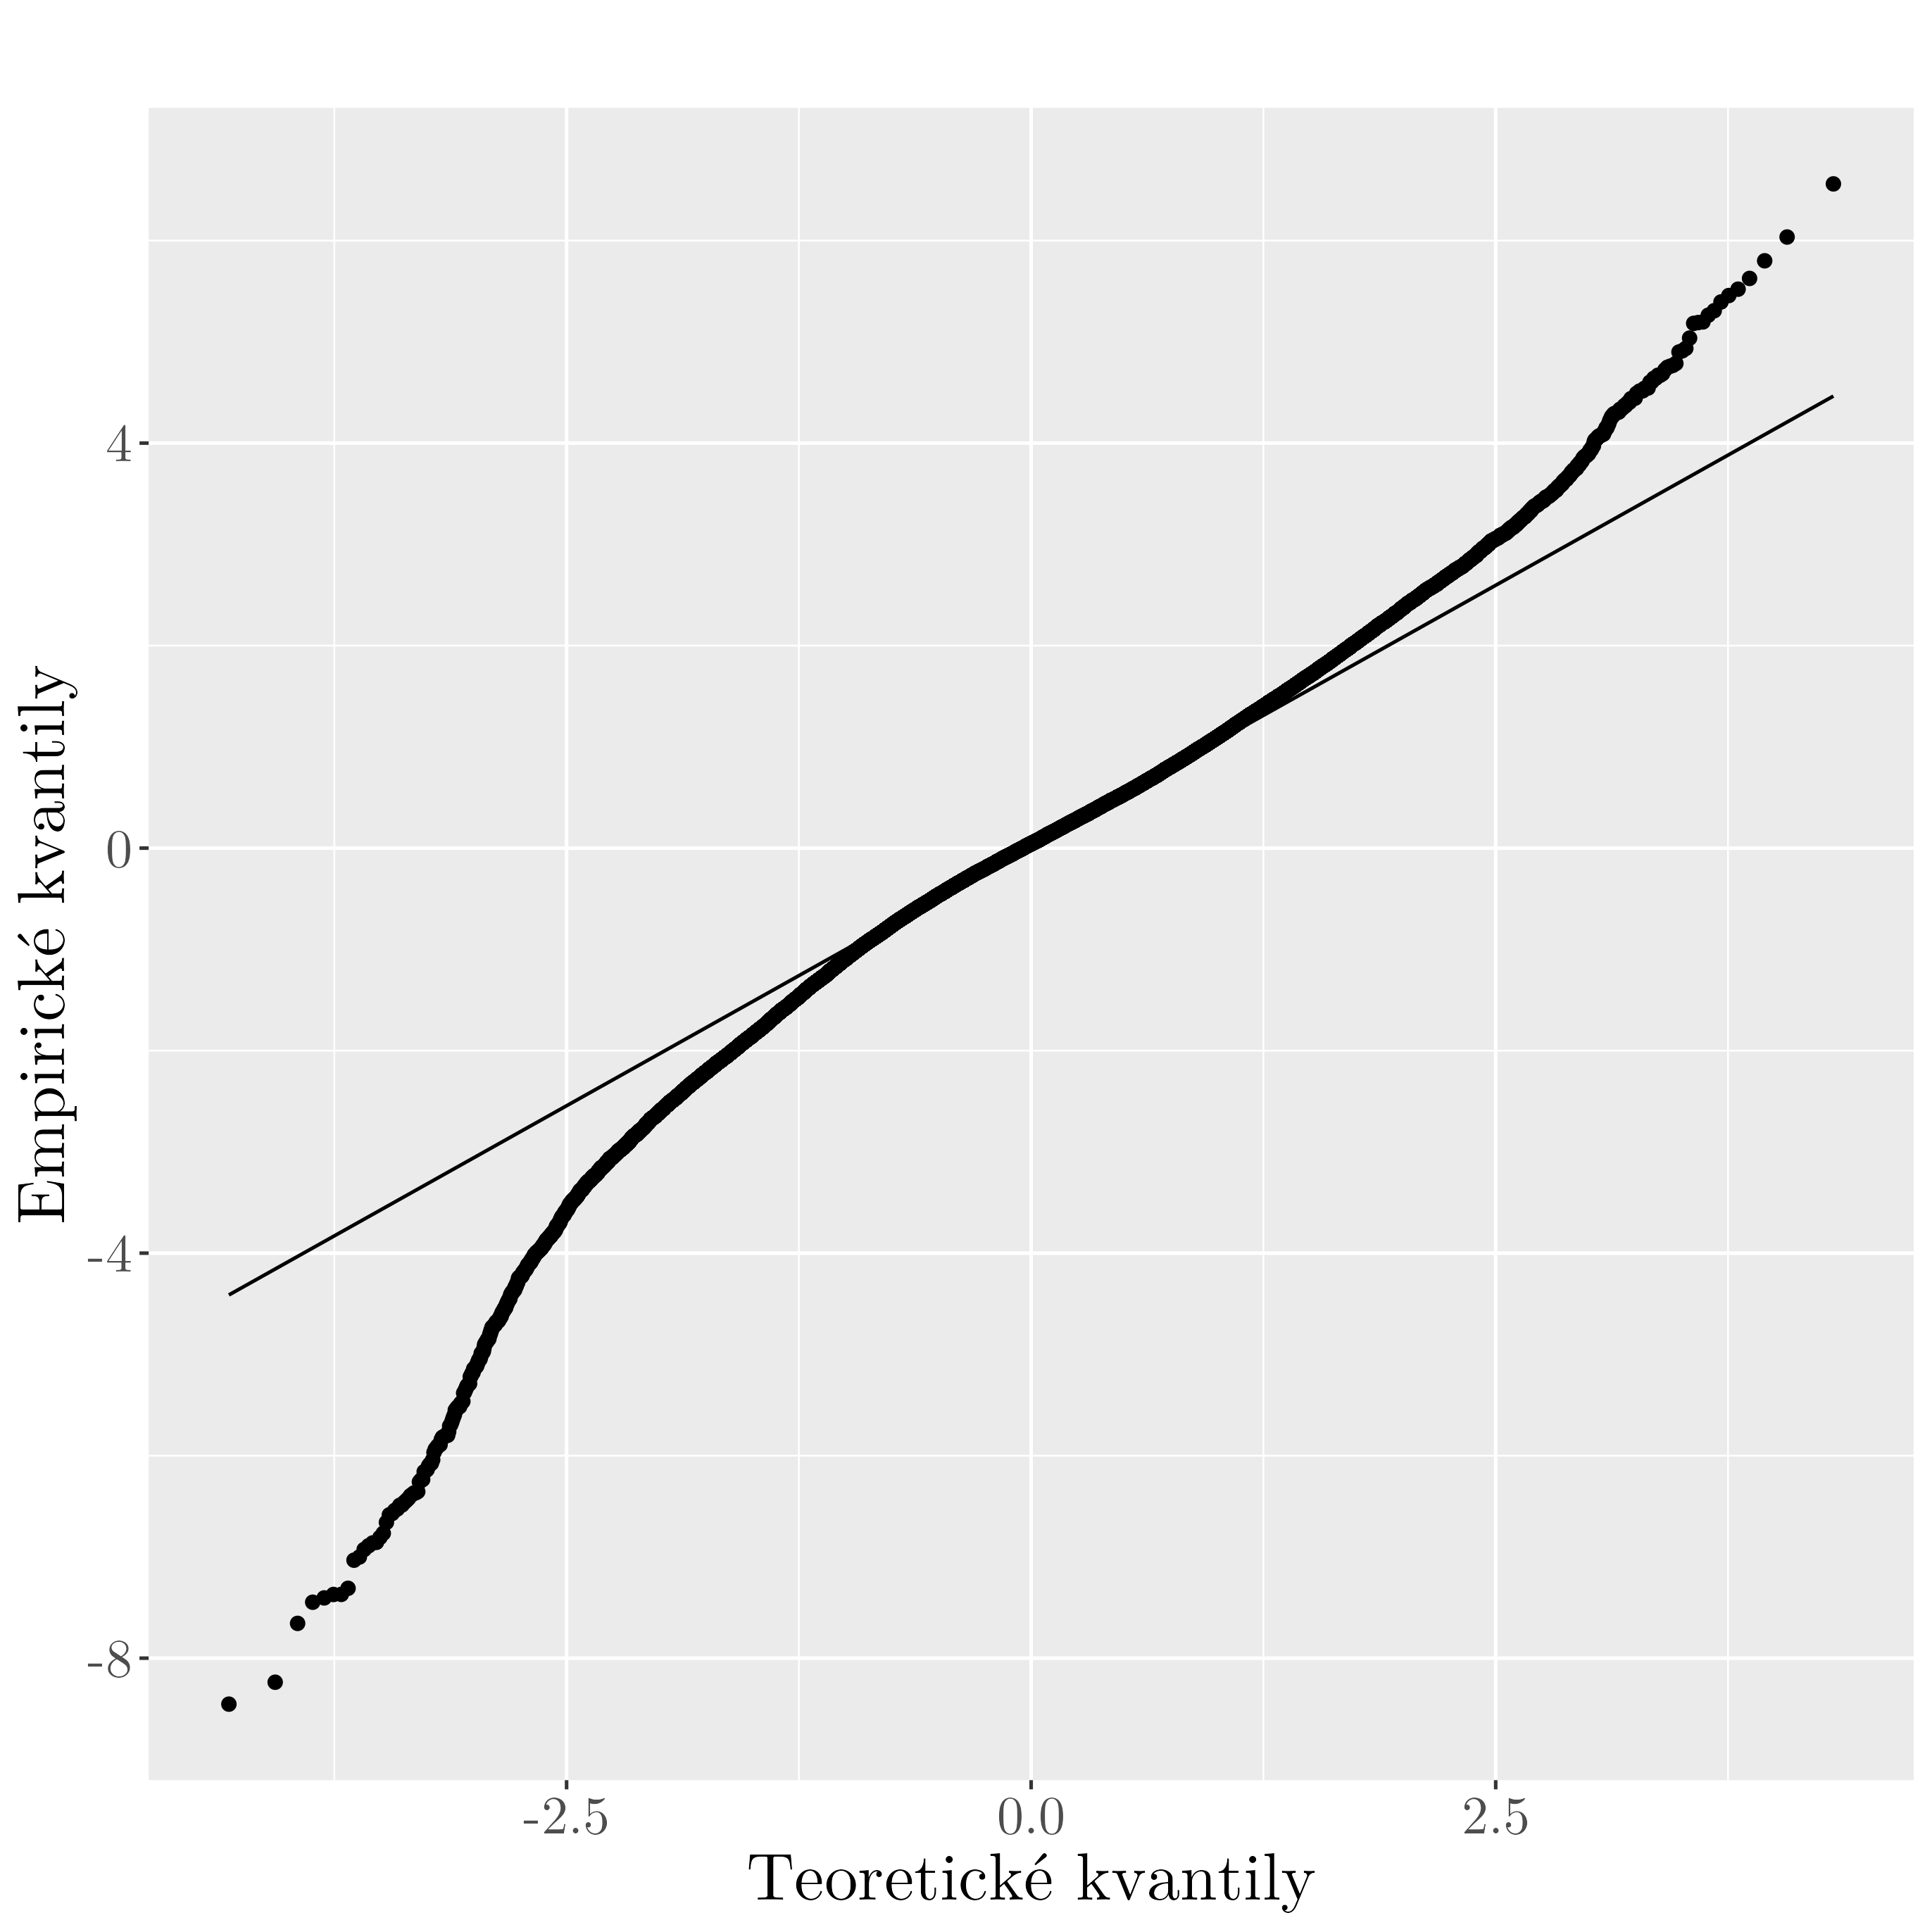
\includegraphics[width=\textwidth]{img/ch2/qq_modmax15cm_sqrt.png}
		\caption{Druhá odmocnina}
		\label{fig:qq_sqrt}
	\end{subfigure}
	\hfill
	\begin{subfigure}{0.45\textwidth}
  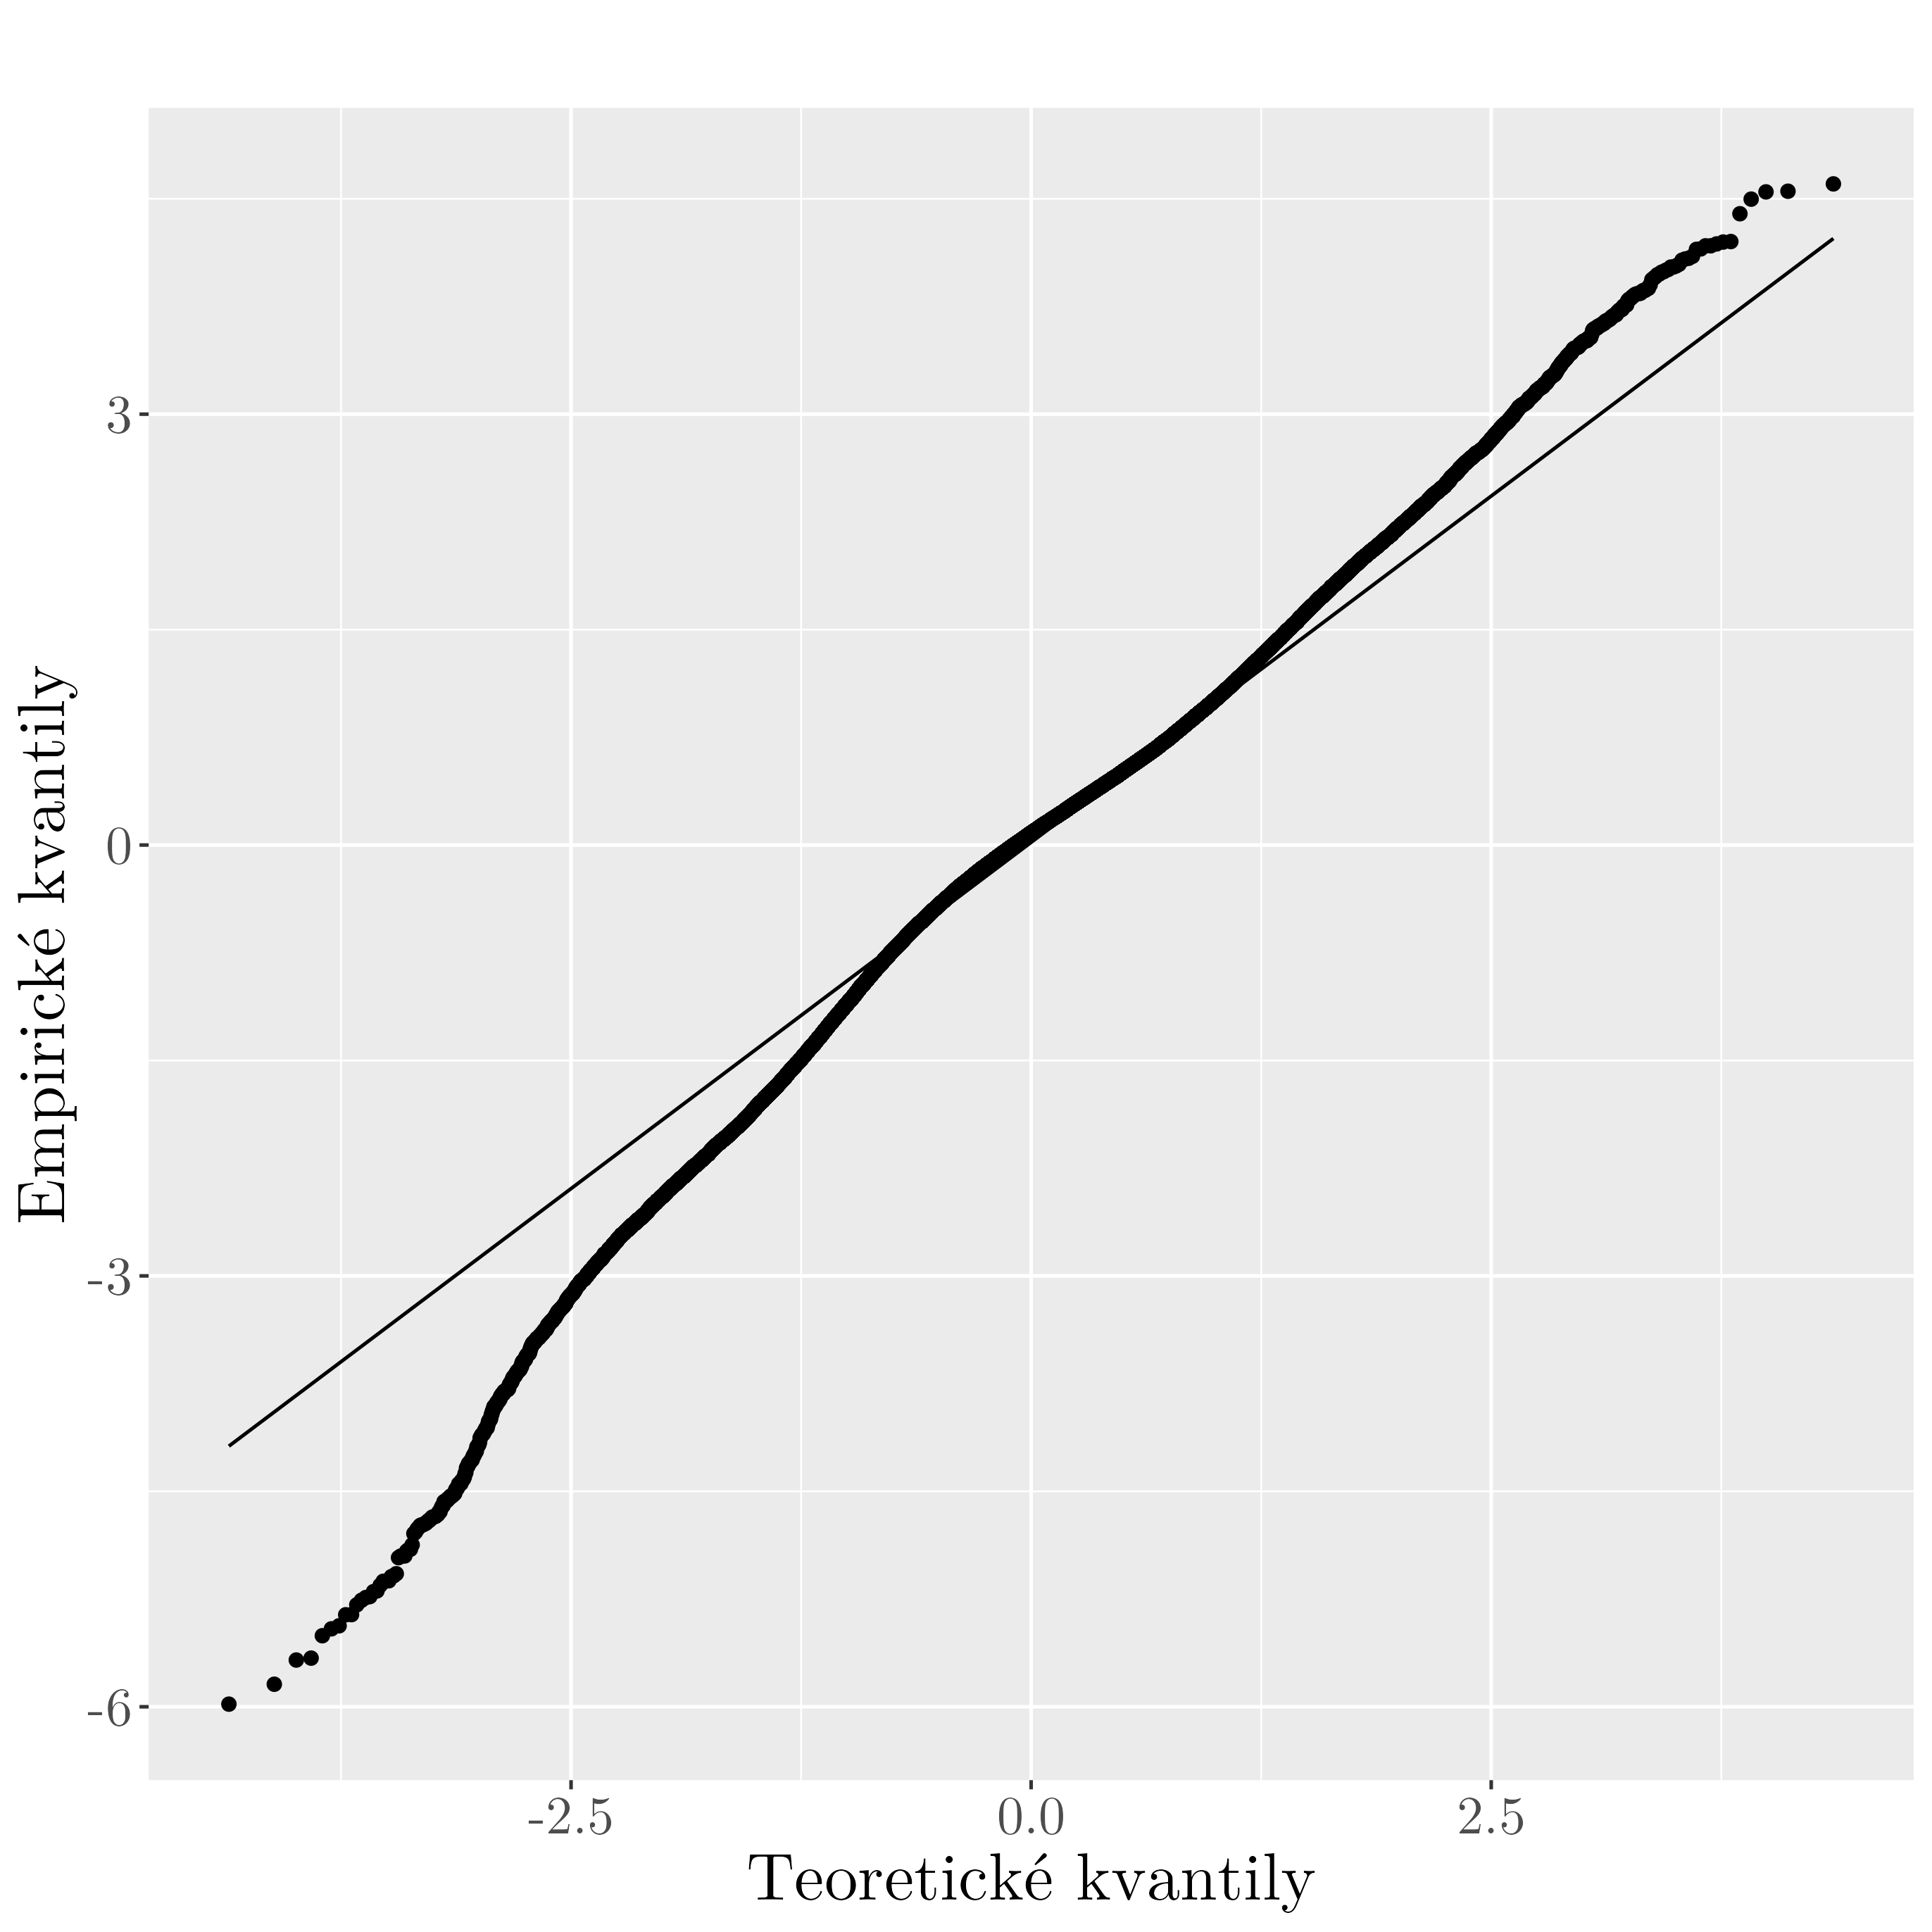
\includegraphics[width=\textwidth]{img/ch2/qq_modmax15cm_curt.png}
		\caption{Třetí odmocnina}
		\label{fig:qq_curt}
	\end{subfigure}
	\caption{Kvantil-kvantilový graf pro jednotlivé transformace vysvětlované proměnné.}
	\label{fig:qq}
\end{figure}

Vidíme, že nejlépe normálnímu rozdělení odpovídá transformace logaritmu a proto s ní budeme nadále pracovat. Na obrázku \ref{fig:resvsfit_log} můžeme vidět srovnání residuálů modelu s fitovanými hodnotami. Diagonálně rozložené body jsou způsobené přítomností faktorové veličiny oblačnosti v modelu. Kromě toho můžeme vidět, že v takto transformovaných datech není výrazná heteroskedasticita.

\begin{figure}
	\centering
  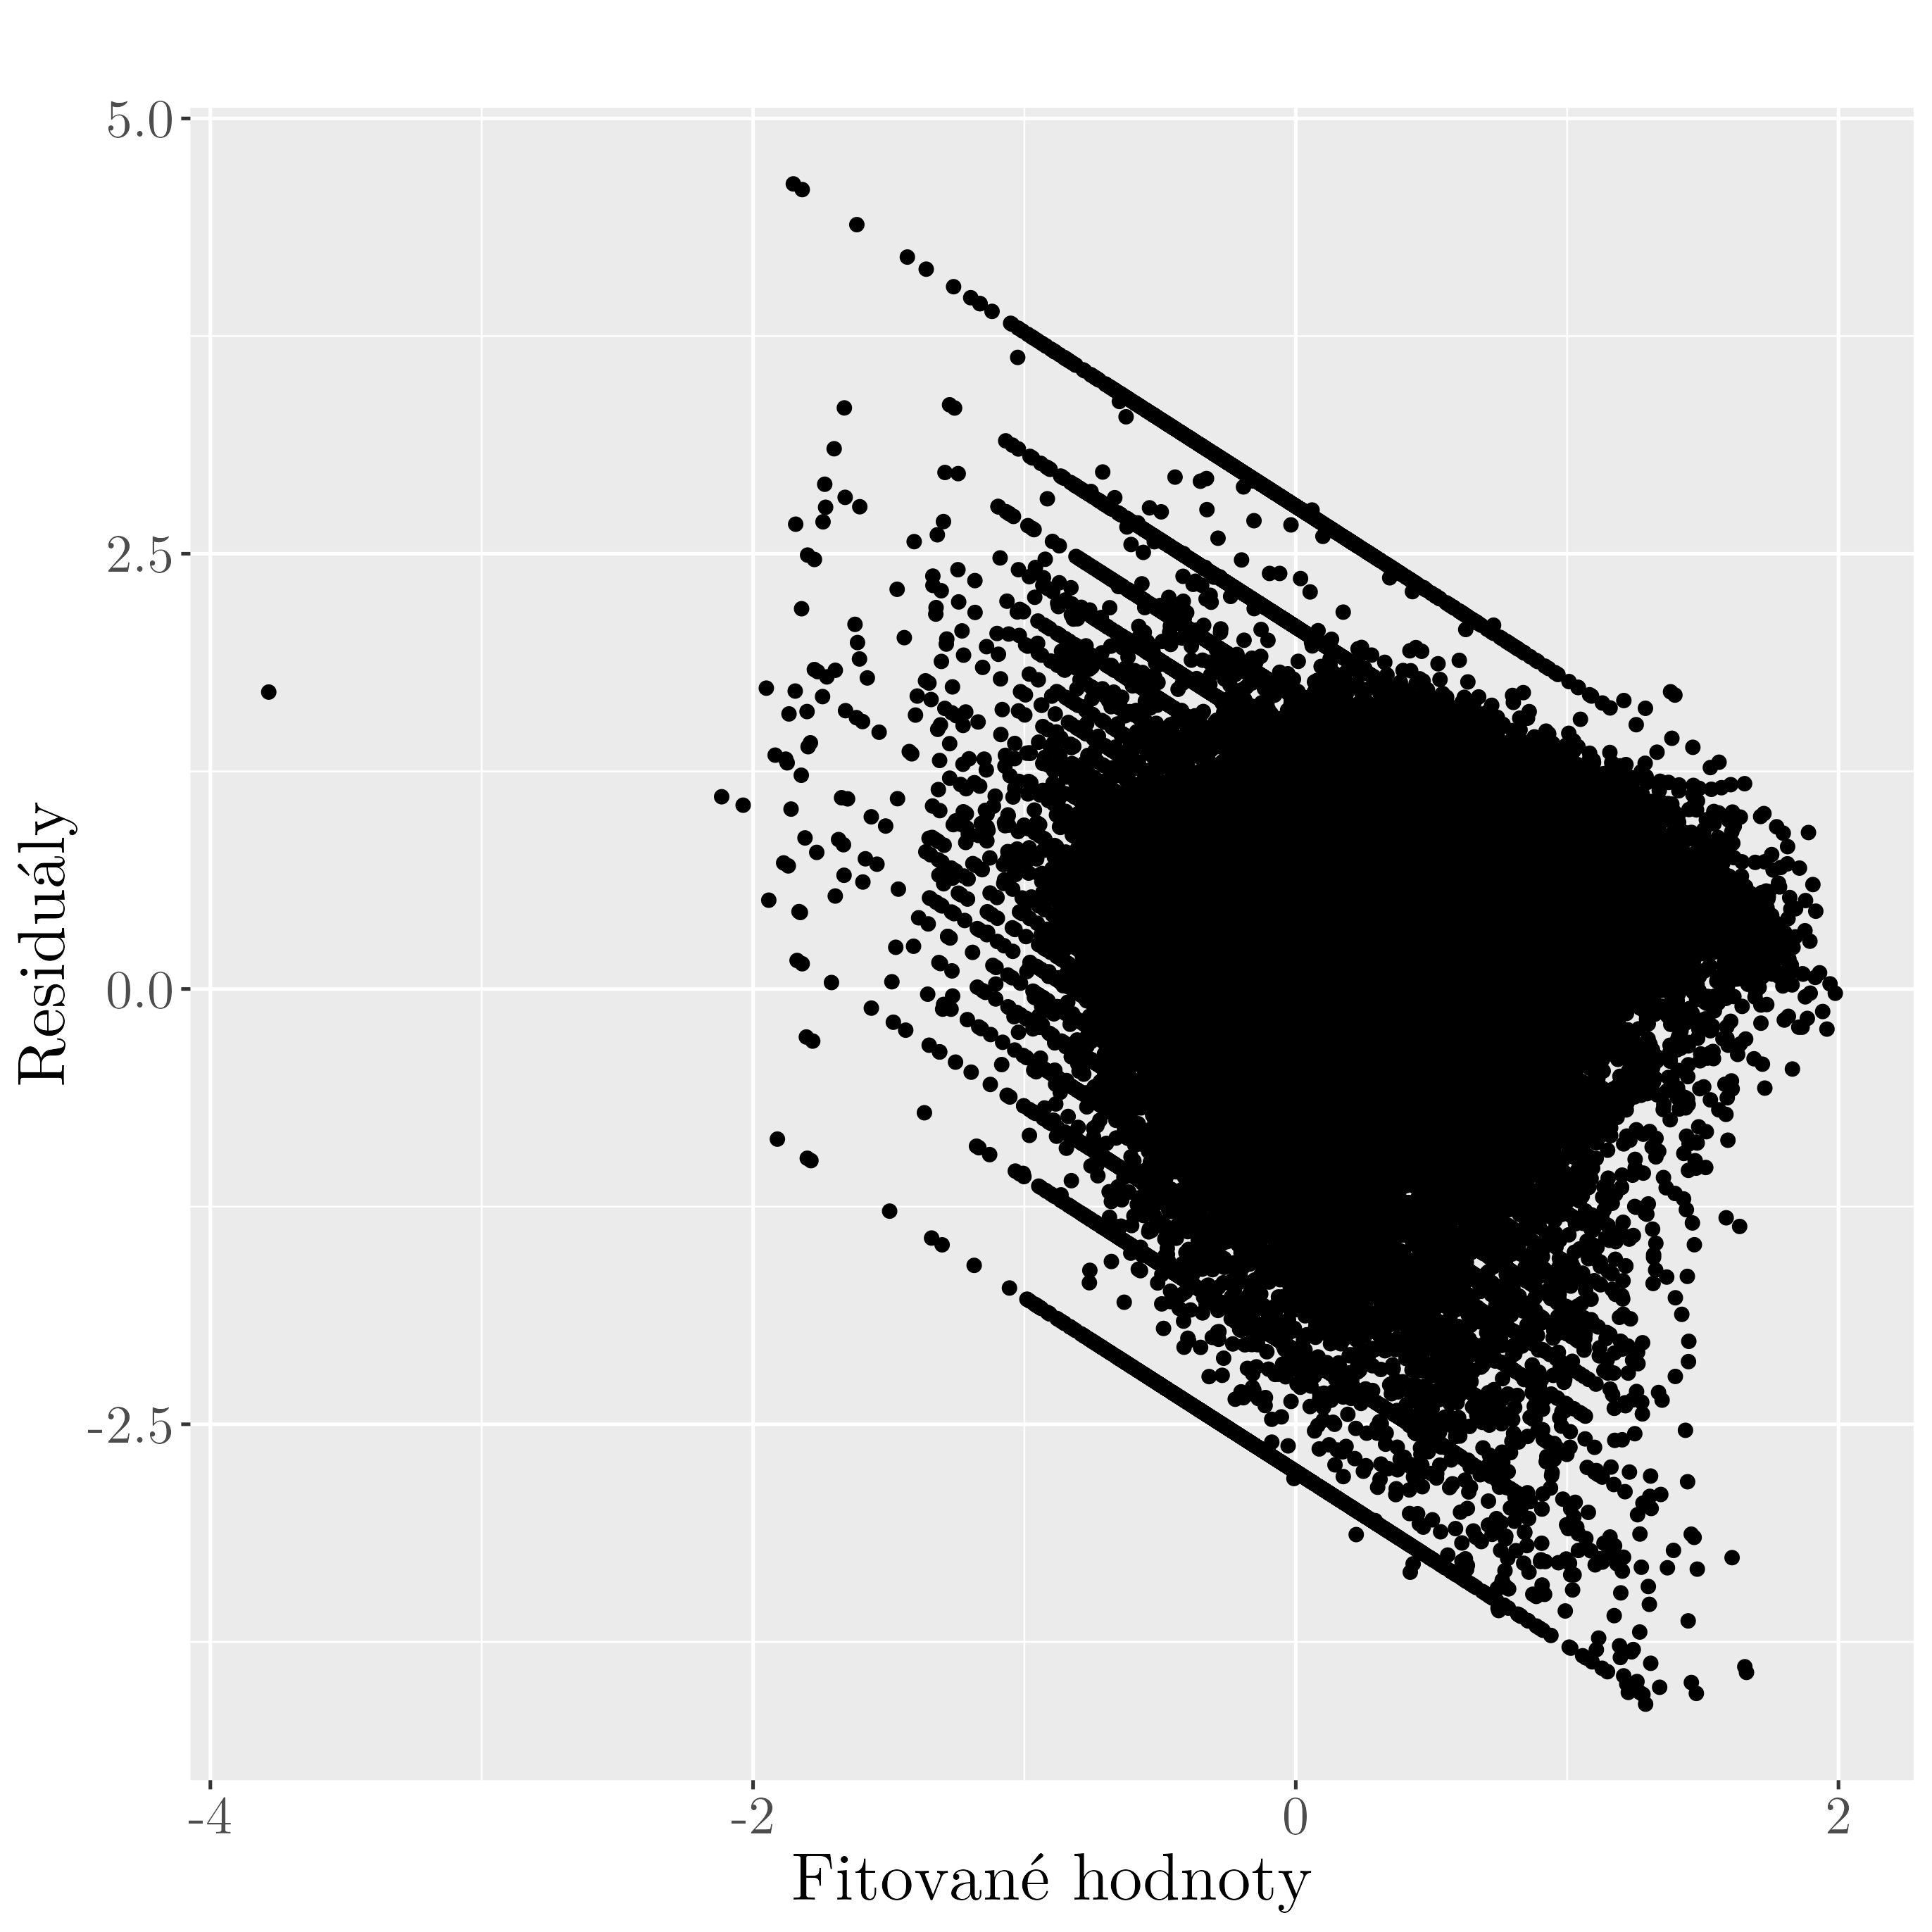
\includegraphics[width=0.55\textwidth]{img/ch2/modmax15cm_log.png}
	\caption{Srovnání residuálů modelu s fitovanými hodnotami pro transformaci pomocí přirozeného logaritmu.}
	\label{fig:resvsfit_log}
\end{figure}

